%%%%%%%%%%%%%%%%%%%%%%%%%%%%%%%%%%%%%%%%%
% Masters/Doctoral Thesis 
% LaTeX Template
% Version 2.5 (27/8/17)
%
% This template was downloaded from:
% http://www.LaTeXTemplates.com
%
% Version 2.x major modifications by:
% Vel (vel@latextemplates.com)
%
% This template is based on a template by:
% Steve Gunn (http://users.ecs.soton.ac.uk/srg/softwaretools/document/templates/)
% Sunil Patel (http://www.sunilpatel.co.uk/thesis-template/)
%
% Template license:
% CC BY-NC-SA 3.0 (http://creativecommons.org/licenses/by-nc-sa/3.0/)
%
%%%%%%%%%%%%%%%%%%%%%%%%%%%%%%%%%%%%%%%%%

%----------------------------------------------------------------------------------------
%	PACKAGES AND OTHER DOCUMENT CONFIGURATIONS
%----------------------------------------------------------------------------------------

\documentclass[
12pt, % The default document font size, options: 10pt, 11pt, 12pt
%oneside, % Two side (alternating margins) for binding by default, uncomment to switch to one side
english, % ngerman for German
onehalfspacing, % Single line spacing, alternatives: onehalfspacing or doublespacing
%draft, % Uncomment to enable draft mode (no pictures, no links, overfull hboxes indicated)
%nolistspacing, % If the document is onehalfspacing or doublespacing, uncomment this to set spacing in lists to single
%liststotoc, % Uncomment to add the list of figures/tables/etc to the table of contents
%toctotoc, % Uncomment to add the main table of contents to the table of contents
%parskip, % Uncomment to add space between paragraphs
%nohyperref, % Uncomment to not load the hyperref package
headsepline, % Uncomment to get a line under the header
%chapterinoneline, % Uncomment to place the chapter title next to the number on one line
%consistentlayout, % Uncomment to change the layout of the declaration, abstract and acknowledgements pages to match the default layout
]{MastersDoctoralThesis} % The class file specifying the document structure

\usepackage[utf8]{inputenc} % Required for inputting international characters
\usepackage[T1]{fontenc} % Output font encoding for international characters

\usepackage{mathpazo} % Use the Palatino font by default
\usepackage{acro} 
%\usepackage[backend=bibtex,style=authoryear,natbib=true]{biblatex} % Use the bibtex backend with the authoryear citation style (which resembles APA)
\usepackage[backend=bibtex,style=alphabetic,
citestyle=authoryear,natbib=true]{biblatex}
%\usepackage[backend=biber,style=alphabetic,]{biblatex}
\addbibresource{example.bib} % The filename of the bibliography

\usepackage[autostyle=true]{csquotes} % Required to generate language-dependent quotes in the bibliography
\usepackage{bm}
\usepackage{amsmath,amssymb,amsfonts}
%\usepackage{algorithmic}
\usepackage[ruled,vlined]{algorithm2e}
\usepackage{neuralnetwork}
\usepackage{array}
\usepackage{bm}
\usepackage{graphicx}
\DeclareAcronym{CT}{
	short=CT,
	long=computed tomography,
}
\DeclareAcronym{FC}{
	short=FC,
	long=fully connected,
}
\DeclareAcronym{ACRIN}{
	short=ACRIN,
	long=American College of Radiology Imaging Network ,
}

\DeclareAcronym{GT}{
	short=GT,
	long=ground truth,
}
\DeclareAcronym{SD}{
	short=SD,
	long=standard deviation,
}
\DeclareAcronym{MLP}{
	short=MLP,
	long=multi-layer perceptron,
}
\DeclareAcronym{SGD}{
	short=SGD,
	long=stocastic gradient dscent,
}
\DeclareAcronym{PReLU}{
	short=PReLU,
	long=parametric rectified linear unit ,
}
\DeclareAcronym{ReLU}{
	short=ReLU,
	long=rectified linear unit ,
}
\DeclareAcronym{DUGAN}{
	short=DUG,
	long=double U-Net generator,
}
\DeclareAcronym{GAN}{
	short=GAN,
	long=generative adversarial network,
}
\DeclareAcronym{ANN}{
	short=ANN,
	long=artificial neural networks,
}
\DeclareAcronym{SSIM}{
	short=SSIM,
	long=structural similarity index,
}
\DeclareAcronym{MAE}{
	short=MAE,
	long=mean absolute error,
}
\DeclareAcronym{RMSE}{
	short=RMSE,
	long=root mean squared error,
}
\DeclareAcronym{MSE}{
	short=MSE,
	long=mean squared error,
}
\DeclareAcronym{PET}{
	short=PET,
	long=positron emission tomography,
}
\DeclareAcronym{SPECT}{
	short=SPECT,
	long=single photon emission computed tomography,class = {in},
}
\DeclareAcronym{MRI}{
	short=MRI,
	long=magnetic resonance imaging,class = {in},
}
\DeclareAcronym{DnCNN}{
	short=DnCNN,
	long=denoising convolutional
	neural network ,
}

\DeclareAcronym{ROI}{
	short=ROI,
	long=region of interest,
	long-plural-form = regions of interest,
}

\DeclareAcronym{SNR}{
	short=SNR,
	long=signal-to-noise ratio,
}

\DeclareAcronym{MLEM}{
	short=MLEM,
	long=maximum likelihood expectation-maximization,
}		
\DeclareAcronym{MBIR}{
	short=MBIR,
	long=model-based iterative reconstruction,
}	

\DeclareAcronym{XCAT}{
	short=XCAT,
	long=extended cardiac-torso,
}

\DeclareAcronym{GPU}{
	short=GPU,
	long=graphical processing unit,
}

\DeclareAcronym{CNN}{
	short=CNN,
	long=convolutional neural network,	
}

\DeclareAcronym{CNR}{
	short=CNR,
	long=contrast-to-noise ratio,
}	
	
\DeclareAcronym{FDG}{
	short=$^{\text{18}}$F-FDG,
	long=$^{\text{18}}$F-fludeoxyglucose,
}
\DeclareAcronym{FLT}{
	short=FLT,
	long=fluorothymidine ,
}

\DeclareAcronym{SUV}{
	short=SUV,
	long=standardized uptake values,
}

\DeclareAcronym{WLS}{
	short=WLS,
	long=weighted least squared,
}
\DeclareAcronym{TV}{
	short=TV,
	long=total variation,
}
\DeclareAcronym{FOV}{
	short=FOV,
	long= field of view,
}


\DeclareAcronym{4D}{
	short=4-D,
	long=four-dimensional,
	class = {out},
}
\DeclareAcronym{3D}{
	short=3-D,
	long=three-dimensional,
}
\DeclareAcronym{2D}{
	short=2-D,
	long=two-dimensional,
}	
\DeclareAcronym{FBP}{
	short=FBP,
	long=filtered-backprojection,
}
\DeclareAcronym{OSEM}{
	short=OSEM,
	long=ordered-subsets expectation-maximisation,
}

\DeclareAcronym{mumap}{
	short=${\mu}$-map,
	long=attenuation map,
	index=$\boldmu$-map,	
}

\DeclareAcronym{UBO}{
	short=UBO,
	long=\emph{Université de Bretagne Occidentale},
}

\DeclareAcronym{HU}{
	short=HU,
	long=Hounsfield unit,
}	

\DeclareAcronym{SR}{
	short=SR,
	long=Super Resolution,
}
\DeclareAcronym{LOR}{
	short=LOR,
	long=line of response,
}
\DeclareAcronym{LRRCED}{
	short=LRRCED,
	long=low-resolution reconstruction aware convolutional encoder decoder,
}

\DeclareAcronym{CED}{
	short=CED,
	long=convolutional encoder decoder,
}

\DeclareAcronym{PWLS}{
	short=PWLS,
	long=penalized weighted least-squares,
}
\DeclareAcronym{DB}{
	short=DB,
	long=Dense Block,
}
\DeclareAcronym{TU}{
	short=TU,
	long=Transition Up,
}
\DeclareAcronym{TD}{
	short=TD,
	long=Transition Down,
}
\DeclareAcronym{PCED}{
	short=P-CED,
	long=Physics-Aware Convolutional Encoder-Decoder,
}
	

\DeclareAcronym{PSNR}{
	short=PSNR,
	long=peak signal-to-noise ratio ,
}


\DeclareAcronym{Lung}{
	short=Lung-PET-CT-Dx,
	long=Large-Scale CT and PET/CT Dataset for Lung Cancer Diagnosis,
}



\newcommand{\boldmu}{\bm{\mu}}
\newcommand{\muhat}{\hat{\mu}}
\newcommand{\boldmuhat}{\bm{\hat{\mu}}}

\newcommand{\boldx}{\bm{x}}
\newcommand{\xhat}{\hat{x}}
\newcommand{\boldxbar}{\bm{\bar{x}}}
\newcommand{\boldxhat}{\bm{\hat{x}}}

\newcommand{\boldlambda}{\bm{\lambda}}
\newcommand{\lambdahat}{\hat{\lambda}}
\newcommand{\boldlambdahat}{\bm{\hat{\lambda}}}

\newcommand{\boldy}{\bm{y}}
\newcommand{\ybar}{\bar{y}}
\newcommand{\yhat}{\hat{y}}
\newcommand{\boldybar}{\bm{\bar{y}}}
\newcommand{\boldyhat}{\bm{\hat{y}}}



\newcommand{\boldL}{\bm{L}}
\newcommand{\boldP}{\bm{P}}


\newcommand{\bbR}{\mathbb{R}}

%\newcommand{\apriori}{\emph{a~priori}}
%\newcommand{\apost}{\emph{a~posteriori}}

\newcommand{\transp}{^\top}


\newcommand{\boldf}{\bm{F}}



\newcommand{\boldzero}{\bm{0}}


\newcommand{\boldb}{\bm{b}}

\newcommand{\bbar}{\bar{b}}
\newcommand{\boldbbar}{\bar{\bm{b}}}

%\newcommand{\fb}{\hat{\bm{x}}_{1}}
%\newcommand{\fbp}{\hat{\bm{x}}_{2}}

\newcommand{\fb}{{\bm{x}}^+_{1}}
\newcommand{\fbp}{{\bm{x}}^+_{2}}



\newcommand{\boldU}{\bm{U}}



%\newcommand{\apriori}{\emph{a~priori}}
%\newcommand{\apost}{\emph{a~posteriori}}



\newcommand{\AP}[1]{{\color{blue}#1}}
\newcommand{\AB}[1]{{\color{red}#1}}


\newcommand{\eR}{\mathbb{R}}
\newcommand{\range}{\mathcal{R}_{\boldP}}
\newcommand{\nullP}{\mathcal{N}_{\boldP}}
\newcommand{\boldv}{\bm{v}}


\newtheorem{proposition}{Proposition}
\newtheorem{definition}{Definition}



%%%%%%%%%%%%%%%%%%%%%%%%%%%%%%%%%%%%%%%%
\usepackage{tikz} 
\usepackage{pgfplots}
\usepackage[labelformat=simple]{subcaption}
\renewcommand\thesubfigure{(\alph{subfigure})}
\usepackage{pifont}% http://ctan.org/pkg/pifont
\newcommand{\cmark}{\ding{51}}%
\newcommand{\xmark}{\ding{55}}%

%----------------------------------------------------------------------------------------
%	MARGIN SETTINGS
%----------------------------------------------------------------------------------------

\geometry{
	paper=a4paper, % Change to letterpaper for US letter
	inner=2.5cm, % Inner margin
	outer=3.8cm, % Outer margin
	bindingoffset=.5cm, % Binding offset
	top=1.5cm, % Top margin
	bottom=1.5cm, % Bottom margin
	%showframe, % Uncomment to show how the type block is set on the page
}

%----------------------------------------------------------------------------------------
%	THESIS INFORMATION
%----------------------------------------------------------------------------------------

\thesistitle{Tomographic Image Reconstruction with Neural Networks} % Your thesis title, this is used in the title and abstract, print it elsewhere with \ttitle
\supervisor{Dr. Dimitris \textsc{Visvikis},\\ Dr. Alexandre Bousse} % Your supervisor's name, this is used in the title page, print it elsewhere with \supname
\examiner{} % Your examiner's name, this is not currently used anywhere in the template, print it elsewhere with \examname
\degree{Doctor of Philosophy} % Your degree name, this is used in the title page and abstract, print it elsewhere with \degreename
\author{Venkata Sai Sundar \textsc{Kandarpa}} % Your name, this is used in the title page and abstract, print it elsewhere with \authorname
\addresses{} % Your address, this is not currently used anywhere in the template, print it elsewhere with \addressname

\subject{Biologie Santé} % Your subject area, this is not currently used anywhere in the template, print it elsewhere with \subjectname
\keywords{} % Keywords for your thesis, this is not currently used anywhere in the template, print it elsewhere with \keywordnames
\university{\href{http://www.university.com}{Université de Bretagne Occidentale}} % Your university's name and URL, this is used in the title page and abstract, print it elsewhere with \univname
\department{\href{http://department.university.com}{Biologie Santé}} % Your department's name and URL, this is used in the title page and abstract, print it elsewhere with \deptname
\group{\href{http://researchgroup.university.com}{LATIM}} % Your research group's name and URL, this is used in the title page, print it elsewhere with \groupname
\faculty{\href{http://faculty.university.com}{Biologie Santé}} % Your faculty's name and URL, this is used in the title page and abstract, print it elsewhere with \facname

\AtBeginDocument{
\hypersetup{pdftitle=\ttitle} % Set the PDF's title to your title
\hypersetup{pdfauthor=\authorname} % Set the PDF's author to your name
\hypersetup{pdfkeywords=\keywordnames} % Set the PDF's keywords to your keywords
}

\begin{document}

\frontmatter % Use roman page numbering style (i, ii, iii, iv...) for the pre-content pages

\pagestyle{plain} % Default to the plain heading style until the thesis style is called for the body content

%----------------------------------------------------------------------------------------
%	TITLE PAGE
%----------------------------------------------------------------------------------------

\begin{titlepage}
\begin{center}

\vspace*{.06\textheight}
{\scshape\LARGE \univname\par}\vspace{1.5cm} % University name
\textsc{\Large Doctoral Thesis}\\[0.5cm] % Thesis type

\HRule \\[0.4cm] % Horizontal line
{\huge \bfseries \ttitle\par}\vspace{0.4cm} % Thesis title
\HRule \\[1.5cm] % Horizontal line
 
\begin{minipage}[t]{0.4\textwidth}
\begin{flushleft} \large
\emph{Author:}\\
\href{http://www.johnsmith.com}{\authorname} % Author name - remove the \href bracket to remove the link
\end{flushleft}
\end{minipage}
\begin{minipage}[t]{0.4\textwidth}
\begin{flushright} \large
\emph{Supervisor:} \\
\href{http://www.jamessmith.com}{\supname} % Supervisor name - remove the \href bracket to remove the link  
\end{flushright}
\end{minipage}\\[3cm]
 
\vfill

\large \textit{A thesis submitted in fulfillment of the requirements\\ for the degree of \degreename}\\[0.3cm] % University requirement text
\textit{in the}\\[0.4cm]
\groupname\\\deptname\\[2cm] % Research group name and department name
 
\vfill

{\large \today}\\[4cm] % Date
%\includegraphics{Logo} % University/department logo - uncomment to place it
 
\vfill
\end{center}
\end{titlepage}

%----------------------------------------------------------------------------------------
%	DECLARATION PAGE
%----------------------------------------------------------------------------------------

\begin{declaration}
\addchaptertocentry{\authorshipname} % Add the declaration to the table of contents
\noindent I, \authorname, declare that this thesis titled, \enquote{\ttitle} and the work presented in it are my own. I confirm that:

\begin{itemize} 
\item This work was done wholly or mainly while in candidature for a research degree at this University.
\item Where any part of this thesis has previously been submitted for a degree or any other qualification at this University or any other institution, this has been clearly stated.
\item Where I have consulted the published work of others, this is always clearly attributed.
\item Where I have quoted from the work of others, the source is always given. With the exception of such quotations, this thesis is entirely my own work.
\item I have acknowledged all main sources of help.
\item Where the thesis is based on work done by myself jointly with others, I have made clear exactly what was done by others and what I have contributed myself.\\
\end{itemize}
 
\noindent Signed:\\
\rule[0.5em]{25em}{0.5pt} % This prints a line for the signature
 
\noindent Date:\\
\rule[0.5em]{25em}{0.5pt} % This prints a line to write the date
\end{declaration}

\cleardoublepage

%----------------------------------------------------------------------------------------
%	QUOTATION PAGE
%----------------------------------------------------------------------------------------

\vspace*{0.2\textheight}

\noindent\enquote{\itshape Thanks to my solid academic training, today I can write hundreds of words on virtually any topic without possessing a shred of information, which is how I got a good job in journalism.}\bigbreak

\hfill Dave Barry

%----------------------------------------------------------------------------------------
%	ABSTRACT PAGE
%----------------------------------------------------------------------------------------

\begin{abstract}
\addchaptertocentry{\abstractname} % Add the abstract to the table of contents
Neural Networks are extensively used in the field of medical imaging for biomedical image segmentation, cancer diagnosis, image analysis, etc. The advancements in computation power (GPUs) and efficient memory utilization have propelled the spread of deep neural networks into various domains. The main motivation behind the use of neural network approaches is faster prediction (compared to traditional methods) without compromising on the quality of the result. Tomographic image reconstruction has also benefited from the development of neural networks. Medical image reconstruction involves the task of mapping raw measurement data collected by the detector to images that are comprehensible to a radiologist. A medical image reconstruction algorithm essentially approximates this mapping to predict the best possible image. There are established analytical and iterative reconstruction algorithms which have over the years proven to be effective in producing the best image possible. Convolutional neural networks (CNN) specifically have proven to be exceptional in tasks related to images such as denoising, deblurring, and super-resolution. The use of neural networks in Positron Emission Tomography (PET) and Computed Tomography (CT) reconstruction has been explored in this thesis. Novel frameworks called DUG-RECON (Double U-Net Generator) for PET, CT image reconstruction, and LRR-CED (Low-Resolution Reconstruction aware Convolutional Encoder-Decoder) for Sparse-view CT image reconstruction and Total-Body PET image reconstruction are proposed in this manuscript. Quantitative analysis of the images reconstructed with the proposed methods indicated that image quality was either better or on par with standard reconstruction algorithms.
\end{abstract}

%----------------------------------------------------------------------------------------
%	ACKNOWLEDGEMENTS
%----------------------------------------------------------------------------------------

\begin{acknowledgements}
\addchaptertocentry{\acknowledgementname} % Add the acknowledgements to the table of contents
The acknowledgments and the people to thank go here, don't forget to include your project advisor\ldots
\end{acknowledgements}

%----------------------------------------------------------------------------------------
%	LIST OF CONTENTS/FIGURES/TABLES PAGES
%----------------------------------------------------------------------------------------

\tableofcontents % Prints the main table of contents

\listoffigures % Prints the list of figures

\listoftables % Prints the list of tables

%----------------------------------------------------------------------------------------
%	ABBREVIATIONS
%----------------------------------------------------------------------------------------

\begin{abbreviations}{ll} % Include a list of abbreviations (a table of two columns)

\textbf{LAH} & \textbf{L}ist \textbf{A}bbreviations \textbf{H}ere\\
\textbf{WSF} & \textbf{W}hat (it) \textbf{S}tands \textbf{F}or\\

\end{abbreviations}

%----------------------------------------------------------------------------------------
%	PHYSICAL CONSTANTS/OTHER DEFINITIONS
%----------------------------------------------------------------------------------------

\begin{constants}{lr@{${}={}$}l} % The list of physical constants is a three column table

% The \SI{}{} command is provided by the siunitx package, see its documentation for instructions on how to use it

Speed of Light & $c_{0}$ & \SI{2.99792458e8}{\meter\per\second} (exact)\\
%Constant Name & $Symbol$ & $Constant Value$ with units\\

\end{constants}

%----------------------------------------------------------------------------------------
%	SYMBOLS
%----------------------------------------------------------------------------------------

\begin{symbols}{lll} % Include a list of Symbols (a three column table)

$a$ & distance & \si{\meter} \\
$P$ & power & \si{\watt} (\si{\joule\per\second}) \\
%Symbol & Name & Unit \\

\addlinespace % Gap to separate the Roman symbols from the Greek

$\omega$ & angular frequency & \si{\radian} \\

\end{symbols}

%----------------------------------------------------------------------------------------
%	DEDICATION
%----------------------------------------------------------------------------------------

\dedicatory{For/Dedicated to/To my\ldots} 

%----------------------------------------------------------------------------------------
%	THESIS CONTENT - CHAPTERS
%----------------------------------------------------------------------------------------
% Chapter Template

\chapter*{Introduction} % Main chapter title
%\addcontentsline{toc}{chapter}{Introduction}
\addcontentsline{toc}{chapter}{\protect\numberline{}Introduction}
\label{Introduction} % Change X to a consecutive number; for referencing this chapter elsewhere, use \ref{ChapterX}

%----------------------------------------------------------------------------------------
%	SECTION 1
%----------------------------------------------------------------------------------------

\section{Motivation}

The use of deep learning in medical imaging has been on the rise over the last few years. It has widely been used in various tasks across medical imaging such as image segmentation  (\cite{ronneberger2015u,guo2019deep,sinha2019multi,dolz2018hyperdense,hatt2018first}), image denoising (\cite{kadimesetty2018convolutional,li2020sacnn,chen2017low,yang2018low}), image analysis (\cite{litjens2017survey,amyar20193,cui2018artificial}). %\noteAB{Add more references}. 
Deep learning based algorithms produce faster results along with best possible quality in accordance with existing state of the art methods (\cite{leuschner2021quantitative}). Medical image reconstruction too has benefited hugely with the advancement of deep learning (\cite{reader2020deep,zhang2020review}).
Medical image reconstruction corresponds to the task of mapping raw projection data retrieved from the detector to image domain data. During the course of this thesis, the focus has been towards \ac{PET} and \ac{CT} image reconstruction. Both these modalities present a unique of set of challenges for image reconstruction. 
 
\ac{PET} imaging is a form of emission tomography wherein the image reconstruction task revolves around identifying the radio-tracer distribution emitted from the patient. A \ac{PET} image gives functional information about the organs in a patient making it invaluable for oncology. Some of the challenges in \ac{PET} image reconstruction are scatter, attenuation and difficulty in identifying the exact annihilation point of the electron-positron. Despite being the most sensitive emission tomography modality, the number of photons captured is low relative to the photons emitted contributing to further image degradation. These challenges result in very noisy images when reconstructed with analytical algorithms. These challenges are addressed by  iterative/model-based approaches which take into account detector geometry, noise statistics and approximate scatter and attenuation correction resulting in better image quality. 

\ac{CT} imaging on the other hand is an example of transmission tomography. The extent of attenuation undergone by X-Rays that pass through a patient are measured to obtain attenuation maps. In \ac{CT} imaging research, there has been active interest in sparse-view and low-dose reconstruction scenarios. In both cases, severe artifacts are introduced in  reconstructed images either due to incomplete projections or low counts. Many established model-based iterative methods account for the low-dose and sparse-view settings to remove artifacts and noise from the reconstruction (\cite{nuyts1998iterative,Elbakri2002,liu2013total}). However, these methods require the knowledge of the noise and artifacts statistics and generally have longer reconstruction times (\cite{kim2014combining}). 


The main tasks involved in image reconstruction can be broadly categorized into three: sinogram correction, domain translation from sinogram to image, and image correction. Algorithms either tackle each of the tasks individually or simultaneously account for them. One can relate to these tasks in the domain of computer vision wherein deep learning architectures have revolutionized the field by producing the state of the art results in most applications (\cite{guo2016deep}). For example, effective use of deep learning-based methods is seen in dealing with image denoising (\cite{kadimesetty2018convolutional,li2020sacnn,chen2017low,yang2018low}), super resolution (\cite{ledig2017photo,lim2017enhanced}) and image-to-image translation tasks (\cite{isola2017image,zhu2017unpaired}). The continuous improvement in the availability of public data has further propelled interest in data-driven medical image reconstruction making it an active area of research. This thesis aims to explore novel deep learning approaches for \ac{PET} and \ac{CT} image reconstruction. Most common ways to introduce deep learning architectures in the image reconstruction pipeline are for pre-processing to correct raw projection data from the detector and post-processing to improve images reconstructed with existing methods. Another way is to embed the network into an iterative algorithm to enable faster convergence. The relatively less explored way called direct image reconstruction is to utilize neural networks alone for the entire reconstruction process. In this thesis two novel \ac{CNN}-based approaches namely \ac{DUGAN}-RECON and \ac{LRRCED} are proposed. The common feature of both these methods is the use of sinogram information to obtain the reconstructed image. The first approach is a direct neural network reconstruction framework that reconstructs images using the sinogram alone as it's input, without any image estimate from traditional methods. It is demonstrated on both \ac{PET} and \ac{CT} data. The second approach utilizes low-resolution \ac{FBP} images along with the sinogram to learn the domain mapping. Although this method is demonstrated on the sparse-view \ac{CT} problem in this manuscript, it can be extended to other modalities too. 


\section{Thesis Organization}

This thesis is divided into six chapters with the first two chapters giving a general introduction to image reconstruction and neural networks respectively. The third chapter presents the relevant literature review, wherein the application and impact of deep learning in image reconstruction research focused on \ac{PET} and \ac{CT} is presented. The next three chapters elaborate the different deep learning-based methods proposed in the thesis.   
In chapter 4, we discuss reconstruction framework \ac{DUGAN} for \ac{PET} and \ac{CT} image reconstruction. A novel method for Sparse-view \ac{CT} reconstruction called \ac{LRRCED} is covered in chapter 5. Potential improvements and ideas for future work are presented in the final chapter. 

%----------------------------------------------------------------------------------------
%	SECTION 3
%----------------------------------------------------------------------------------------

\mainmatter % Begin numeric (1,2,3...) page numbering

\pagestyle{thesis} % Return the page headers back to the "thesis" style

% Include the chapters of the thesis as separate files from the Chapters folder
% Uncomment the lines as you write the chapters

% Chapter Template

\chapter{Introduction} % Main chapter title

\label{Chapter1} % Change X to a consecutive number; for referencing this chapter elsewhere, use \ref{ChapterX}

%----------------------------------------------------------------------------------------
%	SECTION 1
%----------------------------------------------------------------------------------------

\section{Motivation}

The use of deep learning in medical imaging has been on the rise over the last few years. It has widely been used in various tasks across medical imaging such as image segmentation  (\cite{ronneberger2015u,guo2019deep,sinha2019multi,dolz2018hyperdense,hatt2018first}), image denoising (\cite{kadimesetty2018convolutional,li2020sacnn,chen2017low,yang2018low}), image analysis (\cite{litjens2017survey,amyar20193,cui2018artificial}). %\noteAB{Add more references}. 
Deep learning based algorithms produce faster results along with best possible quality in accordance with existing state of the art methods (\cite{leuschner2021quantitative}). Medical Image reconstruction too has benefited hugely with the advancement of deep learning (\cite{reader2020deep,zhang2020review}).
Medical Image reconstruction corresponds to the task of mapping raw projection data retrieved from the detector to image domain data. During the course of this thesis, the focus has been towards \ac{PET} and \ac{CT} image reconstruction. Both these modalities present a unique of set of challenges for image reconstruction. 
 
\ac{PET} imaging is a form of emission tomography wherein the image reconstruction task revolves around identifying the radio-tracer distribution emitted from the patient. A \ac{PET} image gives functional information about the organs in a patient making it invaluable for oncology. Some of the challenges in \ac{PET} image reconstruction are scatter, attenuation and difficulty in identifying the exact annihilation point of the electron-positron. Despite being the most sensitive emission tomography modality, the number of photons captured is low relative to the photons emitted contributing to further image degradation. These challenges result in very noisy images when reconstructed with analytical algorithms. These challenges are addressed by  Iterative/Model-based approaches which take into account detector geometry, noise statistics and approximate scatter and attenuation correction resulting in better image quality. 

\ac{CT} imaging on the other hand is an example of transmission tomography. The extent of attenuation undergone by X-Rays that pass through a patient are measured to obtain attenuation maps. In \ac{CT} imaging research, there has been active interest in sparse-view and low-dose reconstruction scenarios. In both cases, severe artifacts are introduced in  reconstructed images either due to incomplete projections or low counts. Many established model-based iterative methods account for the low-dose and sparse-view settings to remove artifacts and noise from the reconstruction (\cite{nuyts1998iterative,Elbakri2002,liu2013total}). However, these methods for require the knowledge of the noise and artifacts statistics and generally have longer reconstruction times (\cite{kim2014combining}). 


The main tasks involved in image reconstruction can be broadly categorized into three: sinogram correction, domain translation from sinogram to image, and image correction. Algorithms either tackle the three task individually or simultaneously account for them. One can relate to these tasks in the domain of Computer Vision wherein deep learning architectures have revolutionized the field by producing the state of the art results in most applications (\cite{guo2016deep}). For example, effective use of deep learning-based methods is seen in dealing with image denoising (\cite{kadimesetty2018convolutional,li2020sacnn,chen2017low,yang2018low}), super resolution (\cite{ledig2017photo,lim2017enhanced}) and image-to-image translation (\cite{isola2017image,zhu2017unpaired}) tasks. The continuous improvement in the availability of public data has further propelled interest in data-driven medical image reconstruction making it an active area of research. This thesis aims to explore novel deep learning approaches for \ac{PET} and \ac{CT} image reconstruction. Most common ways to introduce deep learning architectures in the image reconstruction pipeline are for pre-processing to correct raw projection data from the detector and post-processing to improve images reconstructed with existing methods. Another way is to embed the network into an iterative algorithm to enable faster convergence. The relatively less explored way called direct image reconstruction is to utilize neural networks alone for the entire reconstruction process. In this thesis \ac{CNN} approaches are proposed for direct image reconstruction with neural networks. 


\section{Thesis Organization}

This thesis is divided into six chapters with the first two chapters being introduction and literature review, followed by three chapters that focus on different deep learning methods explored during the thesis, and finally conclusion and perspectives. In the introduction various aspects of \ac{PET} and \ac{CT} image reconstruction are discussed along with the relevant background in deep learning background. The second chapter throws light on deep learning applied to medical image reconstruction and reviews the state of the art approaches in the scope of this thesis. 
In chapter 3 , we discuss reconstruction framework \ac{DUGAN} for \ac{PET} and \ac{CT} image reconstruction. A novel method for Sparse-view \ac{CT} reconstruction called \ac{LRRCED} is covered in chapter 4. A modified version of \ac{LRRCED} for total body \ac{PET} is discussed in chapter 5. Potential improvements and ideas for future work are presented in the final chapter. 

%----------------------------------------------------------------------------------------
%	SECTION 3
%----------------------------------------------------------------------------------------

\section{Imaging Modalities and Reconstruction}


%-----------------------------------
%	SUBSECTION 1
%-----------------------------------
\subsection{PET}


\ac{PET} images provide functional information to the radiologist making them invaluable in image analysis. The application of \ac{PET} imaging has been on the rise in oncology, cardiology and neuropsychiatry. The increased application lead to the development of many novel reconstruction approaches targeting better image quality. In this section image reconstruction concepts specific to \ac{PET} are discussed. 

The aim of image reconstruction in \ac{PET} is to predict the tracer distribution emitted from the patient. The emission is a result of positron emitting radionuclide injected into the patient which causes positron-electron annihilation. This annihilation results in the production of gamma photons that travel in opposite directions in accordance with the law of conservation of momentum. The simultaneous detection of these photons (also called coincidence events) enables the estimation of tracer distribution in \ac{PET} imaging. A \ac{PET} scanner detects the coincidence events through a set of detectors arranged in a circular fashion. This design of the scanner facilitates detection of coincidence photons between a pair of detectors ($d_p$ and $d_q$). The centers of two detectors are connected by a straight line called \ac{LOR}. Photon pairs that are not subject to scatter are a result of annihilation events that occur along a thin volume surrounding the \ac{LOR}. In \ac{PET}, $\boldx = \boldlambda$ is the distribution of a radiotracer delivered to the patient by injection, and is measured through the detection of pairs of $\gamma$-rays emitted in opposite directions (indirectly from the positron-emitting radiotracer).

\begin{figure}[!htbp]
	\centering
	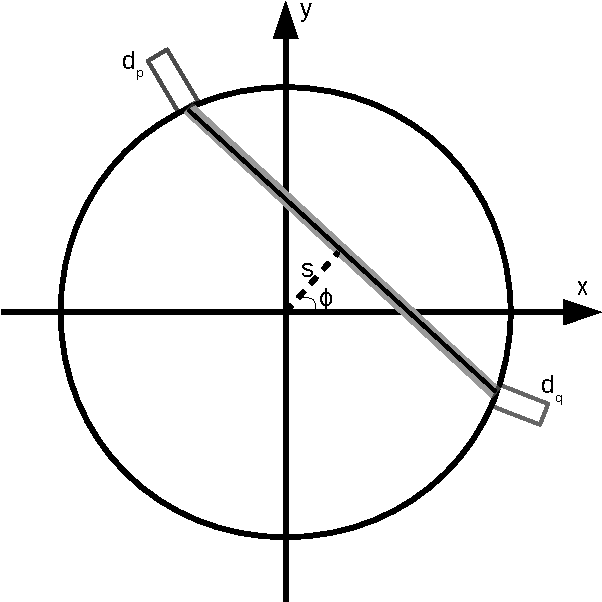
\includegraphics[width=0.6\linewidth]{./Figures/PET_det-crop.pdf}
	\caption{Depiction of a circular \ac{PET} detector with detectors $d_p$ and $d_q$ connected with a \ac{LOR} indicated in gray.}
	\label{fig:2dpet}
\end{figure}

The number of detected coincidence events is related to the \ac{LOR} ($L_{d_{p},d_{q}}$) connecting the centers of detectors $d_p$ and $d_q$ through a sensitivity function $\psi(\vec{r}=(x,y,z))$. It is a Poisson variable whose mean can be written as:

\begin{equation}\label{eq:analy}
\left\langle p_{d_{p},d_{q}}\right\rangle=\tau \int_{\mathrm{FOV}} d \vec{r} \lambda(\vec{r}) \psi_{d_{p}, d_{q}}(\vec{r})
\end{equation}

where $\lambda(\vec{r})$ denotes tracer concentration and $\tau$ is the acquisition time. The tracer concentration is assumed to be contained within the \ac{FOV}. The reconstruction task can be summarized as estimating tracer concentration $\lambda$, given measured data $p_{d_{p},d_{q}}$, $(d_{p},d_{q})=1\dots N_{LOR}$. The above linear model is typically used by analytical algorithms. The measurement data is assumed to have been corrected for non-linear effects like scatter and random coincidences. Another approximation is that $\psi(\vec{r})=0$, except when $r\in L_{d_{p},d_{q}} $. The measured data are therefore modeled as line integrals of tracer distribution ($\lambda$): 

\begin{equation}
\label{eq:line}
\left\langle p_{d_{p}, d_{q}}\right\rangle=\int_{L_{d_{p}, d_{q}}} d \vec{r} \lambda(\vec{r})
\end{equation}

The coincidences from the detector are typically rearranged either in listmode or sinogram format. List mode data is a sequential recording of coincidence events. Time and energy of each detected photon can also be recorded. It has special significance in time of flight imaging for \ac{PET}. Most analytical reconstruction algorithms on the other hand are tailor made for sinogram data format. Fig~\ref{fig:2dpet}, represents a trans-axial slice of a \ac{PET} scanner. One can model 2-D sinogram model with this representation. The variables $s$ and $\phi$ are utilized to relate the \ac{LOR} to the Cartesian co-ordinates $(x,y)$. The radial variable $s$ is the distance between the center of the detector ring and the \ac{LOR}, while angular variable ($\phi$) gives the orientation of the \ac{LOR}. 
For a co-ordinate $t$ along the line, Eq~\ref{eq:line} now becomes:
\begin{equation}\label{eq:line_sino}
\begin{array}{c}
p\left(s, \phi\right)=\int_{\infty}^{\infty} d t \lambda(x= s \cos\phi +t \sin \phi, 
\left.y=s \sin \phi + t \cos \phi\right)
\end{array}
\end{equation}

Through the line integral approximation and keeping in context the corrected \ac{PET} data, $p_{d{a},d_{b}}\approx p(s,\phi)$. The function that maps the tracer distribution onto the line integrals is called as the x-ray transform. It is equivalent to the 2D version of the Radon transform. 


\subsubsection{Analytic Reconstruction}

The starting point of analytic reconstruction is the central slice theorem. It states that 2D Fourier transform of the image ($\Lambda$) is related to the 1D Fourier transform of the x-ray transform as follows:

\begin{equation}
P(v, \phi)=\Lambda\left(v_{x}=v \cos \phi, v_{y}=v \sin \phi\right)
\end{equation} 

where

\begin{equation}
P(v, \phi)=(\mathcal{F} p)(v, \phi)=\int_{\mathbb{R}} d s p(s, \phi) \exp (-2 \pi i s v)
\end{equation}

and $v$ is the frequency variable associated with $s$. In the context of tomographic reconstruction this theorem has the following implication: given the measurement data for all projection angles $\phi \in [0,\pi]$, the radial line sweeps all the frequencies hence making it possible to compute $\Lambda(v_{x},v_{y})$ for $(v_{x},v_{y})\in \mathbb{R}^2$. The image $\lambda$ can then be estimated by finding the inverse 2D Fourier transform. 
One of the most used reconstruction algorithms across modalities is the filtered back-projection algorithm.

\newpage
The version with continuous sampling is written as follows:
 

\begin{equation}
\begin{array}{l}
\lambda(x, y)=\left(X^{*} p^{F}\right)(x, y)= 
\int_{0}^{\pi} d \phi p^{F}(s=x \cos \phi+y \sin \phi, \phi)
\end{array}
\end{equation}


where filtered projections $p^{F}$ are given by

\begin{equation}
p^{F}(s, \phi)=\int_{-R_{F}}^{R_{F}} d s^{\prime} p\left(s^{\prime}, \phi\right) h\left(s-s^{\prime}\right)
\end{equation}


and $h$ is the ramp filter given by

\begin{equation}
h(s)=\int_{-\infty}^{\infty} d v|v| \exp (2 \pi i s v)
\end{equation}



The function mapping from $p^{F}$ to $\lambda$ is the back-projection operator. 
In reality discrete sampling is required to accurately model the acquisition process. The discrete implementation of the \ac{FBP} can be written as follows:

\begin{equation}\label{eq:FBP}
\boldx(i,j) = \frac{\pi}{N_\phi}\sum_{l=0}^{N_\phi-1}\boldy_f(s=i\cos\phi_l+j\sin\phi_l,\phi_l)
\end{equation}

where $x$ is the image for a set of pixels $(i,j)$, $\boldy_f$ are the filtered projections obtained by filtering the projections, expressed in terms of radial variable $s$ and projection angle $\phi$, and $N_\phi$ number of projection angles. The above equation is the approximation of backprojection by a discrete quadrature. 

Analytical methods are faster to implement and practical in a clinical setting but they are vulnerable to noise. The assumptions made in analytical formations are that the measurements are continuous and the solutions are of integral formulation. Sampling is done to the data a posteriori. They are also highly susceptible to system geometry. Since the 80's, \ac{MBIR} techniques \cite{Shepp1982,fessler2000statistical} became the standard approach. They consist in iteratively approximating a solution $\boldxhat$ such that $\boldybar(\boldxhat)$ maximizes the likelihood of the measurement $\boldy$. As they model the stochasticity of the system, they are more robust to noise as compared with \ac{FBP}, and can be completed with a penalty term for additional control over the noise \cite{depierro1995}.


\subsection{Model-based Reconstruction}
The measurement $\boldy$ is a random vector modeling the number of detection (photon counting) at each of the $n$ detector bins, and follows a Poisson distribution with independent entries:
\begin{equation}\label{eq:poisson}
\boldy \sim \mathrm{Poisson}(\boldybar(\boldx))
\end{equation}    
where $\boldybar(\boldx) \in \bbR^n$ is the expected number of counts (noiseless), which is a function of the image $\boldx$. 

The expected number of counts is
\begin{equation}\label{eq:PET}
\boldybar(\boldlambda) = \boldP \boldlambda
\end{equation}
where $\boldP \in \bbR^{n\times m}$ is a system matrix such that each entry $[\boldP]_{i,j}$ represents the probability that a photon pair emitted from voxel $j$. Image reconstruction is achieved by finding a suitable image $\boldxhat = \boldlambdahat$ that approximately solves 
\begin{equation}\label{eq:pb1solve}
\boldy = \boldybar(\boldx) \, .
\end{equation} 


\subsubsection{\ac{MLEM}}
The key components of an iterative method are the data model, cost function and optimization. The cost function for \ac{MLEM} is based on Poisson likelihood given as follows:
\begin{equation}\label{eq:poisson_like}
\operatorname{Pr}\{\boldybar \mid \boldx\}=\prod_{j=1}^{N_{L o R}} \exp \left(-\left\langle y_{j}\right\rangle\right)\left\langle y_{j}\right\rangle^{y_{j}} / y_{j} !
\end{equation}

Putting \ref{eq:PET} in \ref{eq:poisson_like}, taking log and dropping terms that do not depend on unknown image $x$ we get the cost function for \ac{MLEM},

\begin{equation}
Q(\boldxbar, \boldybar)=\sum_{j=1}^{N_{L O R}}\left\{-\sum_{i=1}^{m} P_{j, i} x_{i}+y_{j} \log \left(\sum_{i=1}^{m} P_{j, i} x_{i}\right)\right\}
\end{equation}
where $Q$ is the cost function and the definition of other variables is consistent from above. As long as the matrix $P$ is singular, the above cost function remains convex and results in a unique image. 
The update step to map from the current estimate $x^{n}$ to the next estimate $x^{n+1}$ can be written as follows:

\begin{equation}
\boldxbar_{i}^{n+1}=x_{i}^{n} \frac{1}{\sum_{j^{\prime}=1}^{N_{L o R}} P_{j^{\prime}, i}} \sum_{j=1}^{N_{L O R}} P_{j, i} \frac{y_{j}}{\sum_{i^{\prime}=1}^{m} P_{j, i^{\prime}} x_{i^{\prime}}^{n}} \quad i=1, \ldots, m
\end{equation}

The initial estimate $x_i^{1}$, $i=1, \ldots, m$ typically follows a uniform distribution. The denominator with sum over index $i^{\prime}$ is the forward projection operation. Hence it estimates the measured data for the current image estimate. The numerator with sum over index $j$ is the back projection over the ratio of measured and estimated data. The \ac{MLEM} algorithm does not include a prior and it converges to the image that best fit the data. This estimate has inherent instabilities as the fitting is done closely to the noisy measured data. Various strategies like adding a Bayesian prior to the cost function, filtering the measured data or image post reconstruction, are employed to improve image quality. 


%-----------------------------------
%	SUBSECTION 2
%-----------------------------------
\subsection{CT}
% Write a paragraph on CT imaging

\ac{CT} imaging is a form of transmission tomography. When X-rays are passed through an object they suffer attenuation due to scatter and absorption. Different materials exhibit different absorption properties hence have unique linear attenuation co-efficient. A typical \ac{CT} imaging setup consists of a X-ray source, the object to be imaged and detectors to measure the extent of attenuation experienced by the X-rays. Over the years many imaging geometries have been developed to maximize detector efficiency and obtain better image quality. Fan beam geometry depicted in Fig~\ref{fig:xgeo} was utilized in the experiments undertaken in this thesis. 

\begin{figure}[!htbp]
	\centering
	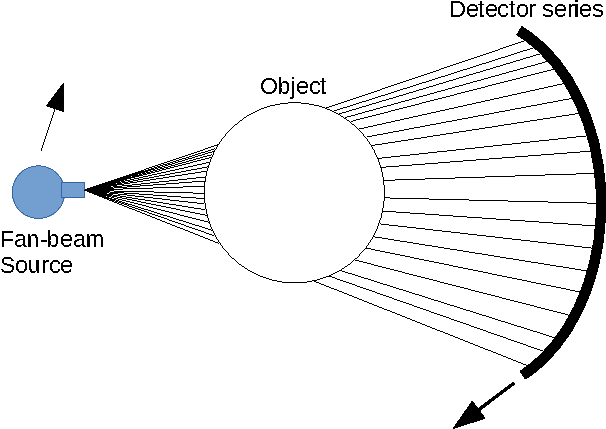
\includegraphics[width=0.7\linewidth]{./Figures/x_ray_geo-crop.pdf}
	\caption{Fan-beam geometry }
	\label{fig:xgeo}
\end{figure}


Let an image be represented by $\boldx \in \bbR^m$ and the scanner measurement by $\boldb \in \bbR^n$ where $m$ is the number of voxels and $n$ is the number of measurements. In \ac{2D} \ac{CT} imaging $n$ depends on the number of detectors $N_\mathrm{d}$ and the number of angles $N_\mathrm{a}$. The task of medical image reconstruction corresponds to finding a mapping from $\boldb$ to $\boldx$. The measurement $\boldb$ is a random vector modeling the number of detection (photon counting) at each of the $n$ detector bins, and follows a Poisson distribution with independent entries, i.e.,
\begin{equation}\label{eq:pCT}
\boldb \sim \mathrm{Poisson}(\boldbbar(\boldx))
\end{equation}    
where, $\boldb  =  [b_1(\boldx),\dots,b_n(\boldx)]\transp\in \bbR^n$ and $\boldbbar(\boldx)  =  [\bbar_1(\boldx),\dots,\bbar_n(\boldx)]\transp\in \bbR^n$ is the expected number of counts (noiseless), which is a function of the image $\boldx$. 

The image $\boldx\in\mathbb{R}^m$ is a vectorized input image (also referred to as attenuation) representing the measure of X-rays absorbed or scattered as they pass through the patient. In a monochromatic setting, the expected number of counts $\boldbbar(\boldx)$  is given by the Beer-Lambert law, i.e.,
\begin{equation}\label{eq:CT}
\bbar_i(\boldx) = I \cdot \exp (-[\boldP \boldx]_i) \quad \forall i=1,\dots,n 
\end{equation}
where, $I$ is the intensity and $\boldP \in \bbR^{n\times m}$ is a system matrix such that each entry $[\boldP]_{i,j}$ represents the contribution of the $j$-th image voxel to the $i$-th detector. Given the raw projections $\boldbbar$, we take the logarithm as follows
\begin{equation}
y_i = \log\left(\frac{I}{b_i}\right) \quad \forall i=1,\dots,n   
\end{equation}
where we assumed that the intensity $I$ is sufficiently high so that $b_i>0$ for all $i$. Image reconstruction is based on finding a suitable image $\boldxhat$ that approximately solves 
\begin{equation}\label{eq:pb2solve}
\boldy = \boldP \boldxhat 
\end{equation} 
 
where $\boldy  =  [y_1,\dots,y_n]\transp\in \bbR^m$. The reconstruction can also be achieved with more sophisticated iterative techniques that account for the stochastic properties of the measurement \eqref{eq:poisson} \cite{nuyts1998iterative,Elbakri2002}.

In a sparse-view setting, the number of rotation angles of the detector is decreased in order to reduce the radiation passing through the patient. This implies a reduction in the number of projection angles in the measurement $\boldy$.


%-----------------------------------
%	SUBSECTION 3
%-----------------------------------

 
%-----------------------------------
%	SUBSECTION 4
%-----------------------------------
\subsection{Iterative Reconstruction Algorithms}

These algorithms are modeled on discrete representation of measurement and the image. They also incorporate corrections for scatter and are independent of detector geometry. Two different \ac{MBIR} methodologies, namely \ac{MLEM} and \ac{WLS} for \ac{PET} and \ac{CT} image reconstruction respectively, are discussed in this section. 

\subsubsection{\ac{WLS}}

One of the most common iterative techniques for \ac{CT} image reconstruction is the \ac{WLS} method, the image $\xhat$ is estimated by minimizing the following:

\begin{equation}
\hat{x}=\underset{x \succeq 0}{\arg \min } \frac{1}{2}\|y-A x\|_{W}^{2}
\end{equation}

where $W=\operatorname{diag}\left\{w_{i}\right\}$ is the diagonal weighting matrix that constitutes for the variance of each ray and $\|z\|_{W}^{2}=z^{\prime} W z$. Despite the statistical weighting, due to the noise in measurements and ill-conditioned problem of image reconstruction the image estimate will still be noisy. 

An improvement to the above can be brought by finding a balance between the desired a priori characteristics of the image and the data fitting. This balance is realized through a regularized \ac{WLS} cost function:

\begin{equation}
\hat{x}=\underset{x \succeq 0}{\arg \min } \Psi(x), \quad \Psi(x) \triangleq \frac{1}{2}\|y-A x\|_{W}^{2}+\beta R(x)
\end{equation} 


where $R(x)$ is the regularization term, that enforces piece-wise smoothness on the image and $\beta$ the regularization parameter. The usual choice for $R$ is an edge preserving regularizer that penalized the differences between neighboring voxels:

\begin{equation}
R(x)=\sum_{j=1}^{n_{\mathrm{p}}} \sum_{k \in \mathcal{N}_{j}} \psi_{j k}\left(x_{j}-x_{k}\right)
\end{equation}    

where $N_j$ are the set of neighboring indices of the $j^\mathrm{th}$ voxel. $\psi$ is a potential function that controls the penalization of differences in the neighboring voxels.

Sparse-view \ac{CT} image reconstruction problem has been explored during the course of this thesis. Sparse-view \ac{CT} image reconstruction is an under-determined problem due to the limited number of projection data available for reconstruction. In such a scenario stronger forms of regularization like \ac{TV} are utilized. Consider a 2D digital image $x[p,q]$, discrete form of \ac{TV} can be written as:

\begin{equation}
\sum_{p} \sum_{p}|x[p, q]-x[p-1, q]|+|x[p, q]-x[p, q-1]|
\end{equation}    

This is an an-isotropic version of \ac{TV} regularization. Images reconstructed with \ac{TV}, sometimes have inexplicable artifacts due to the fact that the absolute value potential is not differentiable at $0$. 

\section{Neural networks}

Neural networks also known as \ac{ANN} are machine learning algorithms that form the basis of deep learning. They inherit name and structure from neurons in the brain. Biological neurons transmit signals to one another through complex networks. This interconnected networking is realized though various architectures by \ac{ANN}s. Sets of artificial neurons are stacked on top of each other to form a layer. A typical neural network consists of many such layers that are connected to each other. The first layer is called input layer, the final layer is termed output layer and the layers in-between are called hidden layers. A neural network with three hidden layers is depicted in Fig~\ref{fig:nn}. The transmission of data across the nodes or artificial neurons happens through the connections. Each and every node has a specific weight and threshold associated. The output from a node is passed through the connection only if the value is above the threshold. Neural network approaches are data-driven. Their performance improves as they learn through training on a dataset. 

\begin{figure}
	\centering
\begin{neuralnetwork}[height=5]
	\newcommand{\x}[2]{$x_#2$}
	\newcommand{\y}[2]{$\hat{y}_#2$}
	\newcommand{\hfirst}[2]{\small $h^{(1)}_#2$}
	\newcommand{\hsecond}[2]{\small $h^{(2)}_#2$}
	\inputlayer[count=4, bias=true, title=Input\\layer, text=\x]
	\hiddenlayer[count=5, bias=false, title=Hidden\\layer 1, text=\hfirst] \linklayers
	\hiddenlayer[count=4, bias=false, title=Hidden\\layer 2, text=\hsecond] \linklayers
	\hiddenlayer[count=3, bias=false, title=Hidden\\layer 3, text=\hsecond] \linklayers
	\outputlayer[count=2, title=Output\\layer, text=\y] \linklayers
\end{neuralnetwork}
\caption{Depiction of a neural network with an input layer, three hidden layers and an output layer}\label{fig:nn}
\end{figure}


To further understand the working of a neural network, we can imagine each node to be solving the problem of linear regression. For example consider a node with four inputs ($x_i, i=1,2,\dots4$), four weights ($w_i, i=1,2,\dots4$) and a bias:

\begin{equation}
\sum_{i=1}^{m} w_{i} x_{i}+\text { bias }=w_{1} x_{1}+w_{2} x_{2}+w_{3} x_{3}+w_{4} x_{4}+\text { bias }
\end{equation}

The output of the node is the above summation after going through an activation function $a$:
\begin{equation}
\text { output }=a(x)=\left\{\begin{array}{l}
1 \text { if } \sum w_{1} x_{1}+b \geq 0 \\
0 \text { if } \sum w_{1} x_{1}+b<0
\end{array}\right.
\end{equation}
In the above example, the given activation function of this node propagates the value $1$ only when the weighted sum of it's inputs is non-negative. When the condition of an activation function are met the output of this node becomes an input to the node to which it's connected. Due to the process of forwarding values through a network, an \ac{ANN} is also called feed-forward network. Complex networks with multiple layers of these nodes are used in practical tasks. An important category of machine learning task is supervised learning. It involves training a neural network on labeled datasets. The goal of training a neural network is to minimize a cost function that enforces the closeness of predicted and real output labels. During the training the network reorganizes it's weights based on the loss function. This process of updating weights is called optimization. Each update is aimed at reaching a minimum of the loss function. A popular optimization method is gradient descent. It guides the model in the direction of reducing errors to reach an optima. The development of back-propagation (\cite{rumelhart1986learning}) has been instrumental in successful implementation of optimization algorithms for neural networks.  


\subsection{Convolutional Neural Networks}

The neural network depicted in \ref{fig:nn} is an example of densely connected network, where all the neighboring nodes are connected with one another. As the size of data increases (say large image data), and the network becomes more complex, the number of parameters increases exponentially. To address this and also to be more suitable for image data \ac{CNN}s were formulated. \ac{CNN}s are extensively used in computer vision tasks like image classification, object detection, image segmentation (\cite{voulodimos2018deep}). The three main building blocks of a \ac{CNN} are Convolution, Activation and Pooling. Each of these layers are discussed below:

\subsection{Convolution}

Images are digitally stored in the form of 2D or 3D matrices depending on the format. A convolution kernel (also known as filter) is a matrix that operates on these images and transforms them based on the kernel values. These kernel values are also known as weights in the neural network terminology. Typically, the size of the kernel is much smaller than that of the image. Many sets of these kernels form the convolution layer of the \ac{CNN}.  The movement of the kernel over the image can be made either by a single pixel or multiple pixels. This step size is called stride ($s$). The resulting output of a convolution between filter and image is called a feature map. Consider a kernel $h$ and input image $f$ with $m$ rows and $n$ columns. Convolution between $h$ and $f$ results in a feature map $g$: 
\begin{equation}
g[m, n]=(h * f)[m, n]=\sum_{i} \sum_{j} h[i, j] f[m-i, n-j]
\end{equation}

\begin{figure}[!htbp]
	\centering
	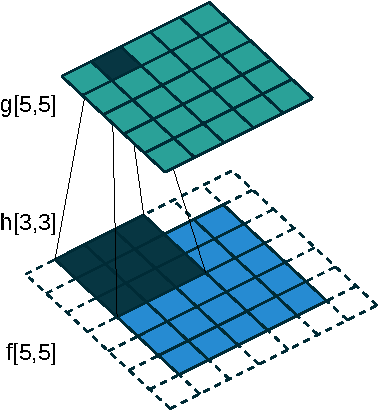
\includegraphics[width=0.4\linewidth]{./Figures/convol-crop.pdf}
	\caption{Convolution of an input image of dimensions 5$\times$5 with a filter of dimensions 3$\times$3.(\cite{dumoulin2016guide})}
	\label{fig:conv}
\end{figure}

Given in Fig~\ref{fig:conv} is a representation of the convolution operation. Zero padding is used to manipulate the dimensions of the feature maps. In the above Figure above it is indicated with dotted lines. The function of padding here is to maintain same dimensions in the input image $f$ and the feature map $g$. A \ac{CNN} learns features from the input through many convolutional layers. The earlier layers learn general features like edges, contrast, the deep layers learn more abstract and finer details.  

\subsection{Activation Layer}

The activation layer that follows the convolution layer in a \ac{CNN} is most commonly the \ac{ReLU} activation function, depicted in Fig~\ref{fig:relu}.

\begin{figure}[!htbp]
	\centering
	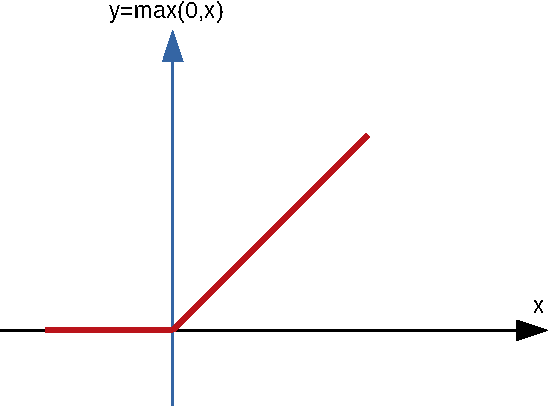
\includegraphics[width=0.6\linewidth]{relu-crop.pdf}
	\caption{The \ac{ReLU} function}
	\label{fig:relu}
\end{figure}


Many of the task based on images are non-linear in nature. Whether a computer vision task like identifying objects in an image or a medical imaging task involving tumor detection, the relationships are far from being linear. The \ac{ReLU} function increases this required non-linearity in the \ac{CNN}. 

\subsection{Pooling Layer}

The third building block of a \ac{CNN} is the pooling layer. Pooling operation is mainly used to reduce the dimensions of a tensor which enables faster computation. Max pooling is the most commonly used pooling operation. A max pooling operator of a particular size returns the maximum value of a selected region in the feature map. Similar to a filter it is implemented with a specific stride. A max pooling filter with $s=2$ is depicted in Fig~\ref{fig:mp}.

\begin{figure}[!htbp]
	\centering
	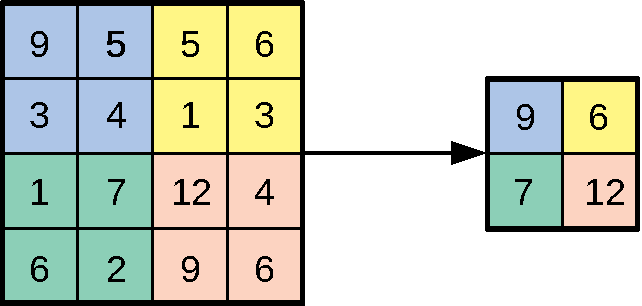
\includegraphics[width=0.6\linewidth]{maxP-crop.pdf}
	\caption{Max pooling with 2$\times$2 filter and stride 1}
	\label{fig:mp}
\end{figure}


A \ac{CNN} with $2$ convolutional layers, $2$ activation layers and $2$ pooling layers is represented in Fig~\ref{fig:trad_cnn}. Layer number is given by $l$. The first and the last layer are the input and output respectively. Usually the last set of layers in a \ac{CNN} used for classification, regression tasks is a fully-connected layer which is similar to the neural network represented in Fig~\ref{fig:nn}. With the advent of powerful computation tools and efficient parallel processing, neural networks with many layers could be implemented. The term deep learning was coined for networks with this "deep" design (\cite{lecun2015deep}). Deep neural networks could be trained over large datasets and they outperformed many existing state of the art algorithms in computer vision. In this thesis we focus specifically on \ac{CNN}s under the umbrella of deep neural networks.  




\begin{figure}[t!]
	\centering
	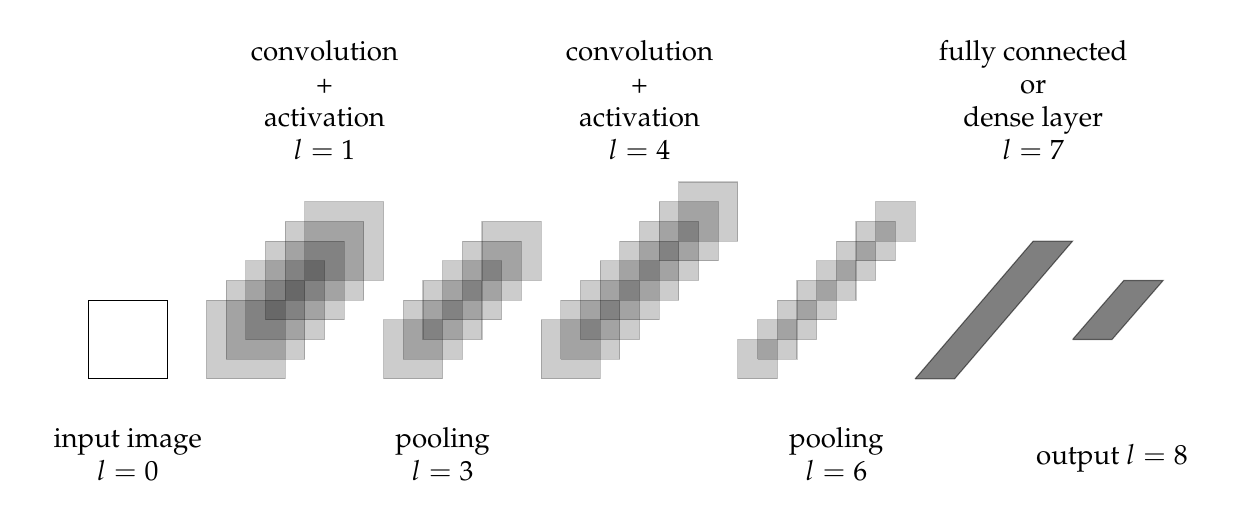
\begin{tikzpicture}
	\node at (0.5,-1){\begin{tabular}{c}input image\\ $l = 0$\end{tabular}};
	
	\draw (0,0) -- (1,0) -- (1,1) -- (0,1) -- (0,0);
	
	\node at (3,3.5){\begin{tabular}{c}convolution \\+\\ activation\\ $l = 1$\end{tabular}};
	
	\draw[fill=black,opacity=0.2,draw=black] (2.75,1.25) -- (3.75,1.25) -- (3.75,2.25) -- (2.75,2.25) -- (2.75,1.25);
	\draw[fill=black,opacity=0.2,draw=black] (2.5,1) -- (3.5,1) -- (3.5,2) -- (2.5,2) -- (2.5,1);
	\draw[fill=black,opacity=0.2,draw=black] (2.25,0.75) -- (3.25,0.75) -- (3.25,1.75) -- (2.25,1.75) -- (2.25,0.75);
	\draw[fill=black,opacity=0.2,draw=black] (2,0.5) -- (3,0.5) -- (3,1.5) -- (2,1.5) -- (2,0.5);
	\draw[fill=black,opacity=0.2,draw=black] (1.75,0.25) -- (2.75,0.25) -- (2.75,1.25) -- (1.75,1.25) -- (1.75,0.25);
	\draw[fill=black,opacity=0.2,draw=black] (1.5,0) -- (2.5,0) -- (2.5,1) -- (1.5,1) -- (1.5,0);
	
	\node at (4.5,-1){\begin{tabular}{c}pooling \\ $l = 3$\end{tabular}};
	
	\draw[fill=black,opacity=0.2,draw=black] (5,1.25) -- (5.75,1.25) -- (5.75,2) -- (5,2) -- (5,1.25);
	\draw[fill=black,opacity=0.2,draw=black] (4.75,1) -- (5.5,1) -- (5.5,1.75) -- (4.75,1.75) -- (4.75,1);
	\draw[fill=black,opacity=0.2,draw=black] (4.5,0.75) -- (5.25,0.75) -- (5.25,1.5) -- (4.5,1.5) -- (4.5,0.75);
	\draw[fill=black,opacity=0.2,draw=black] (4.25,0.5) -- (5,0.5) -- (5,1.25) -- (4.25,1.25) -- (4.25,0.5);
	\draw[fill=black,opacity=0.2,draw=black] (4,0.25) -- (4.75,0.25) -- (4.75,1) -- (4,1) -- (4,0.25);
	\draw[fill=black,opacity=0.2,draw=black] (3.75,0) -- (4.5,0) -- (4.5,0.75) -- (3.75,0.75) -- (3.75,0);
	
	\node at (7,3.5){\begin{tabular}{c}convolution \\+\\ activation\\ $l = 4$\end{tabular}};
	
	\draw[fill=black,opacity=0.2,draw=black] (7.5,1.75) -- (8.25,1.75) -- (8.25,2.5) -- (7.5,2.5) -- (7.5,1.75);
	\draw[fill=black,opacity=0.2,draw=black] (7.25,1.5) -- (8,1.5) -- (8,2.25) -- (7.25,2.25) -- (7.25,1.5);
	\draw[fill=black,opacity=0.2,draw=black] (7,1.25) -- (7.75,1.25) -- (7.75,2) -- (7,2) -- (7,1.25);
	\draw[fill=black,opacity=0.2,draw=black] (6.75,1) -- (7.5,1) -- (7.5,1.75) -- (6.75,1.75) -- (6.75,1);
	\draw[fill=black,opacity=0.2,draw=black] (6.5,0.75) -- (7.25,0.75) -- (7.25,1.5) -- (6.5,1.5) -- (6.5,0.75);
	\draw[fill=black,opacity=0.2,draw=black] (6.25,0.5) -- (7,0.5) -- (7,1.25) -- (6.25,1.25) -- (6.25,0.5);
	\draw[fill=black,opacity=0.2,draw=black] (6,0.25) -- (6.75,0.25) -- (6.75,1) -- (6,1) -- (6,0.25);
	\draw[fill=black,opacity=0.2,draw=black] (5.75,0) -- (6.5,0) -- (6.5,0.75) -- (5.75,0.75) -- (5.75,0);
	
	\node at (9.5,-1){\begin{tabular}{c}pooling\\ $l = 6$\end{tabular}};
	
	\draw[fill=black,opacity=0.2,draw=black] (10,1.75) -- (10.5,1.75) -- (10.5,2.25) -- (10,2.25) -- (10,1.75);
	\draw[fill=black,opacity=0.2,draw=black] (9.75,1.5) -- (10.25,1.5) -- (10.25,2) -- (9.75,2) -- (9.75,1.5);
	\draw[fill=black,opacity=0.2,draw=black] (9.5,1.25) -- (10,1.25) -- (10,1.75) -- (9.5,1.75) -- (9.5,1.25);
	\draw[fill=black,opacity=0.2,draw=black] (9.25,1) -- (9.75,1) -- (9.75,1.5) -- (9.25,1.5) -- (9.25,1);
	\draw[fill=black,opacity=0.2,draw=black] (9,0.75) -- (9.5,0.75) -- (9.5,1.25) -- (9,1.25) -- (9,0.75);
	\draw[fill=black,opacity=0.2,draw=black] (8.75,0.5) -- (9.25,0.5) -- (9.25,1) -- (8.75,1) -- (8.75,0.5);
	\draw[fill=black,opacity=0.2,draw=black] (8.5,0.25) -- (9,0.25) -- (9,0.75) -- (8.5,0.75) -- (8.5,0.25);
	\draw[fill=black,opacity=0.2,draw=black] (8.25,0) -- (8.75,0) -- (8.75,0.5) -- (8.25,0.5) -- (8.25,0);
	
	\node at (12,3.5){\begin{tabular}{c}fully connected\\ or\\ dense layer\\$l = 7$\end{tabular}};
	
	\draw[fill=black,draw=black,opacity=0.5] (10.5,0) -- (11,0) -- (12.5,1.75) -- (12,1.75) -- (10.5,0);
	
	\node at (13,-1){\begin{tabular}{c}output $l = 8$\end{tabular}};
	
	\draw[fill=black,draw=black,opacity=0.5] (12.5,0.5) -- (13,0.5) -- (13.65,1.25) -- (13.15,1.25) -- (12.5,0.5);
	\end{tikzpicture}
	\caption{Architecture of a typical \ac{CNN}. This representation was first proposed by \cite{lecun1995convolutional}.}
	\label{fig:trad_cnn}
\end{figure}

\subsection{Neural Networks for Image Reconstruction}

Image to image translation tasks require the \ac{CNN} to map from image in one domain to an image in another related domain. This requires the design of the \ac{CNN} to be quite different from the one depicted in Fig~\ref{fig:trad_cnn}. Convolution and pooling operations compress the input to obtain an abstract representation in lower dimensions. To transform the output into an image from the lower dimensional representation, transposed convolution operators are used. In contrast to the compressing nature of convolutions, they expand the input feature map. The combination of convolution+pooling and transposed convolutions are adjusted depending on the dimensions of the input and output images. Transposed convolution is shown in Fig~\ref{fig:tc}. Essentially the transposed convolution spatially reverses the dimensions of the convolution+pooling operation. 

\begin{figure}[!htbp]
	\centering
	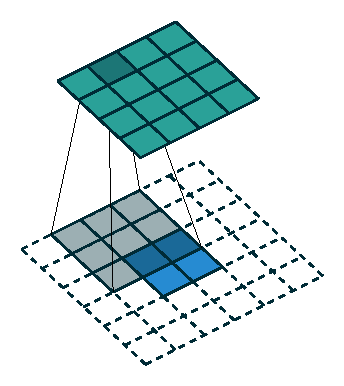
\includegraphics[width=0.5\linewidth]{transposed.pdf}
	\caption{Transposed convolution over a $2\times2$ input to get a $4\times4$ output. (\cite{dumoulin2016guide})}
	\label{fig:tc}
\end{figure}

Transposed convolutions are used in many tasks like super resolution, image segmentation, denoising and image reconstruction. This version of \ac{CNN} appropriate for image reconstruction is represented in Fig~\ref{fig:fcn}

\begin{figure}[!htbp]
	\centering
	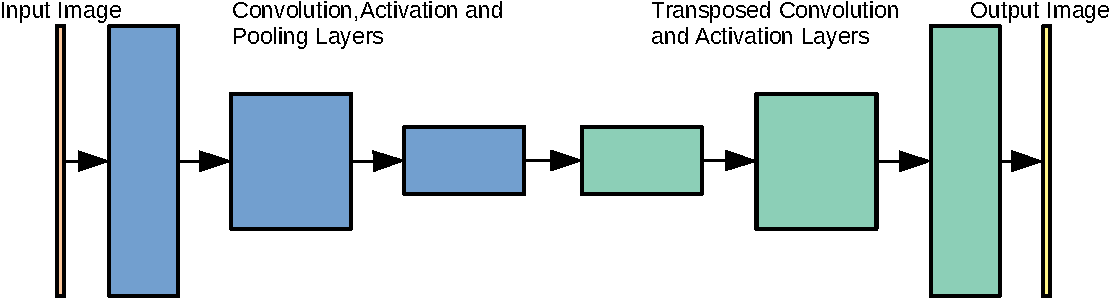
\includegraphics[width=1.0\linewidth]{fcn-crop.pdf}
	\caption{\ac{CNN} for image to image translation tasks. This example has an identical structure in convolution path and the transposed convolution path.}
	\label{fig:fcn}
\end{figure}

These architectures are sometimes referred to as \ac{CED}, since they contain two distinct paths of down sampling of input and up sampling of lower dimensional representation. The building blocks described in this section essentially form the basis of \ac{CNN}s proposed in this thesis. The next chapter consists of a review of existing works in deep learning applied to medical image reconstruction. And the following chapters describe the proposed methods. 




\chapter{Neural Networks} 


\label{Chapter2}

Neural networks, also known as \ac{ANN} are machine learning algorithms that form the basis of deep learning. They inherit name and structure from neurons in the brain. Biological neurons transmit signals to one another through complex networks. This interconnected networking is realized though various combinations of neurons forming an \ac{ANN}. Sets of artificial neurons are stacked on top of each other to form a layer. A typical neural network consists of many such layers that are connected to each other. The first layer is called input layer, the final layer is termed output layer and the layers in-between are called hidden layers. A neural network with three hidden layers is depicted in Fig~\ref{fig:nn}. The transmission of data across the nodes or artificial neurons happens through the connections. Each and every node has a specific weight and threshold associated. The output from a node is passed through the connection only if the value is above the threshold. Neural network approaches are data-driven. Their performance improves as they learn through training on a dataset. 

\begin{figure}
	\centering
\begin{neuralnetwork}[height=5]
	\newcommand{\x}[2]{$x_#2$}
	\newcommand{\y}[2]{$\hat{y}_#2$}
	\newcommand{\hfirst}[2]{\small $h^{(1)}_#2$}
	\newcommand{\hsecond}[2]{\small $h^{(2)}_#2$}
	\inputlayer[count=4, bias=true, title=Input\\layer, text=\x]
	\hiddenlayer[count=5, bias=false, title=Hidden\\layer 1, text=\hfirst] \linklayers
	\hiddenlayer[count=4, bias=false, title=Hidden\\layer 2, text=\hsecond] \linklayers
	\hiddenlayer[count=3, bias=false, title=Hidden\\layer 3, text=\hsecond] \linklayers
	\outputlayer[count=2, title=Output\\layer, text=\y] \linklayers
\end{neuralnetwork}
\caption{Depiction of a neural network with an input layer, three hidden layers and an output layer}\label{fig:nn}
\end{figure}


To further understand the working of a neural network, we can imagine each node to be solving the problem of linear regression. For example consider a node with four inputs ($x_i, i=1,2,\dots4$), four weights ($w_i, i=1,2,\dots4$) and a bias:

\begin{equation}
\sum_{i=1}^{m} w_{i} x_{i}+\text { bias }=w_{1} x_{1}+w_{2} x_{2}+w_{3} x_{3}+w_{4} x_{4}+\text { bias }
\end{equation}

The output of the node is the above summation after going through an activation function $g$:
\begin{equation}
\text { output }=g(x)=\left\{\begin{array}{l}
1 \text { if } \sum w_{1} x_{1}+b \geq 0 \\
0 \text { if } \sum w_{1} x_{1}+b<0
\end{array}\right.
\end{equation}
In the above example, the given activation function of this node propagates the value $1$ only when the weighted sum of it's inputs is non-negative. When the condition of an activation function are met, the output of this node becomes an input to the node to which it's connected. Due to the process of forwarding values through a network, an \ac{ANN} is also called feed-forward network. Complex networks with multiple layers of these nodes are used in practical tasks. An important category of machine learning task is supervised learning. It involves training a neural network on labeled datasets. The goal of training a neural network is to minimize a cost function that enforces the closeness of predicted and real output labels. During the training the network reorganizes it's weights based on the loss function. This process of updating weights is called optimization. Each update is aimed at reaching a minimum of the loss function. A popular optimization method is gradient descent. It guides the model in the direction of reducing errors to reach an optima. The development of back-propagation (\cite{rumelhart1986learning}) has been instrumental in successful implementation of optimization algorithms for neural networks. A machine learning algorithm is typically specified by a cost function, an optimization procedure and a model. Even neural network design is based on these principles. One can find a co-relation between the iterative reconstruction algorithms based on gradient-based optimization and neural network training with gradient descent. It is to be noted that the non-linearity in the activation functions causes moss functions to become non-convex. This implies that gradient-based optimizers used for neural network training essentially drive the cost function to a very small value without a global convergence guarantee. Neural networks are initialized to small random variables prior to training as gradient descent without the convergence guarantee is sensitive to values of initial weights. 
 

\section{Cost Function}

Neural networks can be represented by parametric models that define a distribution $p(\boldsymbol{y} \mid \boldsymbol{x} ; \boldsymbol{\theta})$. The aim is to learn a conditional distribution to predict $\boldsymbol{y}$ given $\boldsymbol{x}$. Through principle of maximum likelihood, cross-entropy between the training data and the model's predictions become the cost function. This negative log-likelihood or cross-entropy between training data and model distribution can be written as:

\begin{equation}\label{eq:log_like}
\mathbf{J}(\boldsymbol{\theta})=-\mathbb{E}_{\mathbf{x}, \mathbf{y} \sim \hat{p}_{\text {data }}} \log p_{\text {model }}(\boldsymbol{y} \mid \boldsymbol{x})
\end{equation}

Given a specific $p_{\text {model}}$, the cost function exhibits a different form. Expanding the above generates some terms which are discarded as they do not depend on trainable model parameters. As an example, if $p_{\text {model}}$ follows a Gaussian distribution $\mathcal{N}(\boldsymbol{y} ; f(\boldsymbol{x} ; \boldsymbol{\theta}), \boldsymbol{I})$, Equation~\ref{eq:log_like} becomes:

\begin{equation}
\mathbf{J}(\theta)=\frac{1}{2} \mathbb{E}_{\mathbf{x}, \mathbf{y} \sim \hat{p}_{\text {data }}}\|\boldsymbol{y}-f(\boldsymbol{x} ; \boldsymbol{\theta})\|^{2}
\end{equation}

The above is equivalent to \ac{MSE} between the model distribution and the training data and is one of the most commonly used loss functions in training neural networks for linear regression. This approach of deriving the cost function from maximum likelihood removes the difficulty of choosing cost functions for each model. Choice of the model itself determines the cost function. Another popular loss function \ac{MAE} can be derived from \ref{eq:log_like} by assuming $p_{\text {model}}$ to follow a Laplacian distribution. 

\section{Output Unit}

Neural networks as described above consists of an output layer after a series of hidden layers. The choice of cost function and output layer are highly dependent on each other. The representation of the output, determines the cross-entropy function. Given a set of hidden features defined by $\boldsymbol{h} = f(x;\boldsymbol{\theta}).$, the role of the output layer is to transform the features appropriate for the task at hand. The most common choices for output layers are linear units and sigmoid units. Given a set of features $h$, a linear layer outputs a vector $\hat{\boldsymbol{y}}=\boldsymbol{W}^{\top} \boldsymbol{h}+\boldsymbol{b}$. A modification of a linear layer is \acf{ReLU} given by $g(z)=\max \{0, z\}$. The frequent usage of linear units is to find the mean of a conditioned Gaussian distribution. For regression tasks the output unit typically has the linear activation. Tasks like binary classification require to define Bernoulli distribution for the maximum likelihood approach. The network needs to predict only $\boldsymbol{P}(y=1 \mid x)$. The output value need to be in the interval $[0,1]$. In this scenario a sigmoid activation does the task of transforming the hidden features into normalized probability value in the range $[0,1]$. A sigmoid output unit is defined by:

   
\begin{equation}
\hat{y}=\sigma\left(\boldsymbol{w}^{\top} \boldsymbol{h}+b\right)
\end{equation}

where $\sigma$ is given by:

\begin{equation}
\sigma(x)=\frac{1}{1+\exp (-x)}
\end{equation}

The hidden units are usually preferred to have \ac{ReLU} or variations of \ac{ReLU} as the activation in order to have significant gradients during optimization. 

\section{Backpropagation}

Consider a feedforward network with an input $\boldsymbol{x}$ that produces an output $\boldsymbol{y}$. The propagation through the network starts with initial information from the inputs and continues through the hidden units at each layer, finally resulting in the output $\hat{\boldsymbol{y}}$. This process is termed as forward propagation. Back-propagation on the other hand makes computes the gradient by making the cost flow backwards through the network. Forward propagation is carried on during training to produce a scalar cost $J(\boldsymbol{\theta})$, which is then utilized by back-propagation to compute the gradients. Back-propagation is a simplified way for computing the gradients and is used with an optimization algorithm like stochastic gradient descent for network training. The most important gradient required in learning algorithms is the one of cost function with respect to learning parameters, $\nabla J(\boldsymbol{\theta})$. 

The neural network given in Fig~\ref{fig:nn} follows computational graph representation. In order to discuss back-propagation, we formulate a simple notation using graphs. Each node in the graph can be considered to be a variable. The variable could be of any type, say a scalar, vector or a matrix. Another component of a computational graph is an operation. It is just a simple function based on one or more variables. An operation is assumed to return a single output variable, which could have single or multiple entries. A simple computational graph with one hidden layer and sigmoid output unit is shown in Fig~\ref{fig:graph}.  

\begin{figure}[!htbp]
	\centering
	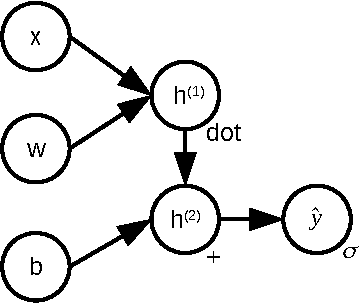
\includegraphics[width=0.4\linewidth]{./Figures/back_prop-crop.pdf}
	\caption{Computational graph with one hidden layer. The nodes in the first layer store the input $x$, weight $w$ and the bias $b$. The second layer contains the hidden layer with 2 units each with the corresponding operation written below. The final layer is the output layer denoted by  $\hat{y}=\sigma(wx+b)$, where $\sigma$ is the sigmoid function defined earlier.}
	\label{fig:graph}
\end{figure}

The gradients in the backpropagation algorithm are calculated by recursively applying the chain rule of calculus. The chain rule is a process of computing derivatives of functions based on multiple functions whose derivatives are already known. Back-propagation is an efficient implementation of chain rule with an order of operations feasible for computation. Let the input $x$,$b$ and $w$ to be real numbers, and $h^{1}$,$h^{2}$ and $\hat{y}$ be functions mapping from one real number to another, the chain rule can be written as follows:

\begin{equation}
\frac{d y}{d x}=\frac{d y}{d h^{2}} \frac{d h^{2}}{d h^{1}} \frac{d h^{1}}{d x}
\end{equation}

where $h^{1}=xw$, $h^{2}=h^{1}+b$ from Figure~\ref{fig:graph}. We can generalize the above for a vector case with $x,w,b \in \mathbb{R}^{m}$ as follows:

\begin{equation}
\frac{\partial y}{\partial x_{i}}=\sum_{j} \frac{\partial y}{\partial h^{1}_{j}} \frac{\partial h^{2}_{j}}{\partial h^{1}_{j}}\frac{\partial h^{1}_{j}}{\partial x_{j}}
\end{equation}

The chain rule involves many repeatable expressions which may need to be stored to avoid multiple re-computations for estimating gradients. Especially for complex neural networks it would lead to an exponentially high number of computations. A simplistic version of the backpropagation algorithm for a fully-connected \ac{MLP} is discussed in this section. For a supervised loss function $L(\hat{\boldsymbol{y}},\boldsymbol{y})$, where $\hat{\boldsymbol{y}}$ is the predicted output and $\boldsymbol{y}$ the target, forward propagation for a single training example is shown in Algorithm~\ref{alg:forward}. After the forward propagation the gradient on the cost function $J$ is calculated and then propagated through the network through back-propagation described in Algorithm~\ref{alg:backprop}. 
\begin{algorithm}
	\SetAlgoLined
	Number of layers, $l$ \;
    Network weights represented by matrices, $\boldsymbol{W}^{(i)},i \in \{1,\dots,l\}$ \;
	Bias parameters, $\boldsymbol{b}^{(i)},i \in \{1,\dots,l\}$ \;
	Hidden units, $h^{(i)}, i \in \{1,\dots,n\}$ \;
    
	$h^{(0)} = \boldsymbol{x} $, \Comment{Initializing input nodes} \;
    
    \For{$j =1,\dots,l$}{
		$a^{(j)}= b^{(j)} + \boldsymbol{W}^{(j)}h^{(j-1)}$ 	\Comment{information from previous layers}\; 
		$h^{(j)}= f(a^{(j)})$                               \Comment{activation in the current layer}\;
		}
	$\hat{\boldsymbol{y}} = h^{(l)}$			\;
	$J = L(\hat{\boldsymbol{y}},\boldsymbol{y}) + \lambda R(\theta)$ \Comment{Cost function with a regularization} \;
	\caption{Forward propagation algorithm for a single input example $\boldsymbol{x}$}
	\label{alg:forward}
\end{algorithm}

\begin{algorithm}
	\SetAlgoLined
	Computing gradient $g$ of the output layer\;
	$g = \nabla_{\hat{\boldsymbol{y}}} J = \nabla_{\hat{\boldsymbol{y}}} L (\hat{\boldsymbol{y}},y) $
	
	\For{$j =l,l-1\dots,1$}{
		The gradient of a particular layer's output needs to be converted into gradient before activation $f$\;
		$g = \nabla_{\boldsymbol{a}^{(j)}} J = g \circ f^{'}(a^{(j)}) $ \;
		Gradients on weights and biases \;
		$\nabla_{b^{(j)}}J = g + \lambda \nabla_{b^{(j)}} R(\theta)$ \;
		$\nabla_{\boldsymbol{W}^{(j)}}J = g h^{(j-1)} + \lambda \nabla_{\boldsymbol{W}^{(j)}} R(\theta)$ \;
		Propagating the gradients through the preceding lower lowel activations\;
		$g = \nabla_{\boldsymbol{h}}J = \boldsymbol{W}^{(j)\intercal}g$
		
	}
	\caption{Backward propagation for neural network from Algorithm~\ref{alg:forward}}
	\label{alg:backprop}
\end{algorithm}

  
\section{Optimization}
Once the gradients are calculated through backpropagation algorithm, optimization procedures like gradient descent can be use to update the network parameters ($\theta$). The two algorithms in the previous section were demonstrated for a single example. In reality neural networks are often trained in parallel on multiple examples. This set of combined examples is called a batch and optimization algorithms are implemented accordingly for training in batches. In this section we discuss two of the most used optimization algorithms \ac{SGD} and ADAM. 

\subsection{Stochastic Gradient Descent}
\ac{SGD} is an implementation of the popular gradient descent algorithm for training in batches. We obtain an estimate of the gradient by averaging the gradient over a minibatch of $m$ training examples taken from the data distribution. \ac{SGD} is depicted in Algorithm~\ref{alg:sgd}.  

\begin{algorithm}
	\SetAlgoLined
	Learning rate $\epsilon_{j}$\;
	Current parameters $\theta_{k}$\;
	\While{stopping criterion is not reached}{
		From the training set, sample $m$ minibatch of examples $\{ \boldsymbol{x}^{(1)},\dots, \boldsymbol{x}^{(m)} \}$ and corresponding targets $\{ \boldsymbol{y}^{(1)},\dots, \boldsymbol{y}^{(m)} \}$ \\
		Computing average gradient: \\
		$\hat{g} = \frac{1}{m} \nabla_{\theta_{j}} \sum_{i=1}^{m} L(f(\boldsymbol{x}^{(i)},\theta_{j}),\boldsymbol{y}^{(i)})$ \\
		Update: $\theta_{j} = \theta_{j} - \epsilon \hat{g} $ \\
		
	}
	\caption{Training update at an iteration $j$ for \acf{SGD}}
	\label{alg:sgd}
\end{algorithm}

The learning rate $\epsilon_{j}$ is gradually decreased as the training progresses, due to the noise introduced by random sampling of minibatches. 

\subsection{Adam}
Adam is another optimization algorithm which incorporates adaptive learning rate and momentum for faster convergence (\cite{kingma2014adam}). Momentum introduces velocity denoted by $v$ that indicates speed and direction for parameters to update through parameter space. It is typically set to an exponentially decaying average of the negative gradient. Adam is derived from adaptive momentum. It is depicted in Algorithm~\ref{alg:adam}.

\begin{algorithm}
	\SetAlgoLined
	Step size $\epsilon$ default usually $0.001$ \;
	Exponential decay rates $\rho_{1}$ and $\rho_{2}$, typically set to $0.9$ and $0.999$ \;
	Constant $\delta$, a very small number for stabilization, usually in the order of $10^{-8}$ \;
    Parameters $\theta$ \;
    $1^{\mathrm{st}}$ and $2^{\mathrm{nd}}$ moment variables, initialized to $s=0$, $r=0$ \;
    Time step $t=0$ \;
    
	\While{stopping criterion is not reached}{
		From the training set, sample $m$ minibatch of examples $\{ \boldsymbol{x}^{(1)},\dots, \boldsymbol{x}^{(m)} \}$ and corresponding targets $\{ \boldsymbol{y}^{(1)},\dots, \boldsymbol{y}^{(m)} \}$ \\
		Computing average gradient: \\
		$\hat{g} = \frac{1}{m} \nabla_{\theta_{j}} \sum_{i=1}^{m} L(f(\boldsymbol{x}^{(i)},\theta_{j}),\boldsymbol{y}^{(i)})$ \\
		$t = t+1$ \\
		Update first momentum estimate: $s = \rho_{1}s + (1-\rho_{1})g $ \\
		Update second momentum estimate: $r = \rho_{2}r + (1-\rho_{2})g \circ g $ \\
		Correct bias in first moment: $\hat{s}= \frac{s}{1-\rho_{1}^{t}}$ \\
		Correct bias in second moment: $\hat{r}= \frac{r}{1-\rho_{2}^{t}}$ \\
		Calculate parameter update: $\Delta \theta_{j} = -\epsilon\frac{\hat{s}}{\sqrt{\hat{r}+\delta}}$\\
		Update:  $\theta = \theta + \Delta \theta$ \\
		
	}
	\caption{Adam algorithm}
	\label{alg:adam}
\end{algorithm}

\section{Convolutional Neural Networks}

The neural network depicted in \ref{fig:nn} is an example of densely connected network, where all the neighboring nodes are connected with one another. As the size of data increases (say large image data), and the network becomes more complex, the number of parameters increases exponentially. To address this and also to be more suitable for image data \ac{CNN}s were formulated. \ac{CNN}s are extensively used in computer vision tasks like image classification, object detection, image segmentation (\cite{voulodimos2018deep}). The three main building blocks of a \ac{CNN} are Convolution, Activation and Pooling. Each of these layers are discussed below:

\subsection{Convolution}

Images are digitally stored in the form of 2D or 3D matrices depending on the format. A convolution kernel (also known as filter) is a matrix that operates on these images and transforms them based on the kernel values. These kernel values are also known as weights in the neural network terminology. Typically, the size of the kernel is much smaller than that of the image. Many sets of these kernels form the convolution layer of the \ac{CNN}.  The movement of the kernel over the image can be made either by a single pixel or multiple pixels. This step size is called stride ($s$). The resulting output of a convolution between filter and image is called a feature map. Consider a kernel $h$ and input image $f$ with $m$ rows and $n$ columns. Convolution between $h$ and $f$ results in a feature map $g$: 
\begin{equation}
g[m, n]=(h * f)[m, n]=\sum_{i} \sum_{j} h[i, j] f[m-i, n-j]
\end{equation}

\begin{figure}[!htbp]
	\centering
	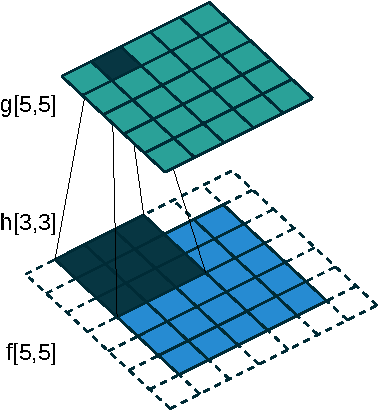
\includegraphics[width=0.4\linewidth]{./Figures/convol-crop.pdf}
	\caption{Convolution of an input image of dimensions 5$\times$5 with a filter of dimensions 3$\times$3.(\cite{dumoulin2016guide})}
	\label{fig:conv}
\end{figure}

Given in Fig~\ref{fig:conv} is a representation of the convolution operation. Zero padding is used to manipulate the dimensions of the feature maps. In the above Figure above it is indicated with dotted lines. The function of padding here is to maintain same dimensions in the input image $f$ and the feature map $g$. A \ac{CNN} learns features from the input through many convolutional layers. The earlier layers learn general features like edges, contrast, the deep layers learn more abstract and finer details.  

\subsection{Activation Layer}

The activation layer that follows the convolution layer in a \ac{CNN} is most commonly the \ac{ReLU} activation function, depicted in Fig~\ref{fig:relu}.

\begin{figure}[!htbp]
	\centering
	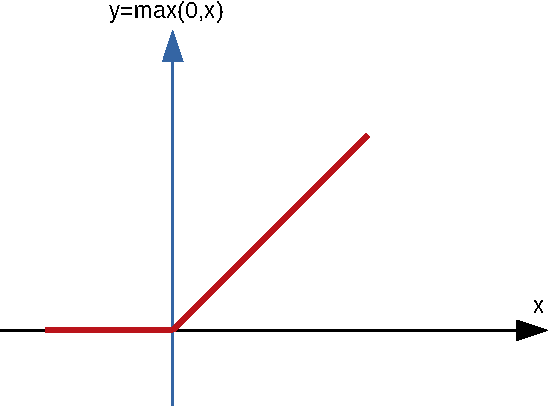
\includegraphics[width=0.6\linewidth]{relu-crop.pdf}
	\caption{The \ac{ReLU} function}
	\label{fig:relu}
\end{figure}


Many of the task based on images are non-linear in nature. Whether a computer vision task like identifying objects in an image or a medical imaging task involving tumor detection, the relationships are far from being linear. The \ac{ReLU} function increases this required non-linearity in the \ac{CNN}. 

\subsection{Pooling Layer}

The third building block of a \ac{CNN} is the pooling layer. Pooling operation is mainly used to reduce the dimensions of a tensor which enables faster computation. Max pooling is the most commonly used pooling operation. A max pooling operator of a particular size returns the maximum value of a selected region in the feature map. Similar to a filter it is implemented with a specific stride. A max pooling filter with $s=2$ is depicted in Fig~\ref{fig:mp}.

\begin{figure}[!htbp]
	\centering
	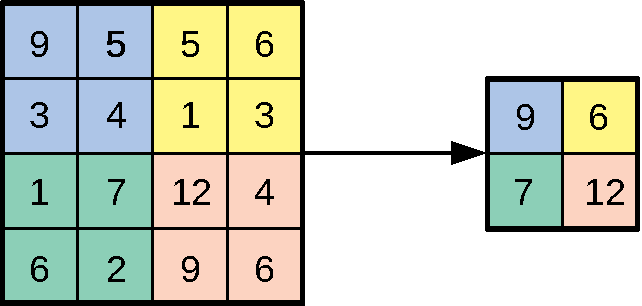
\includegraphics[width=0.6\linewidth]{maxP-crop.pdf}
	\caption{Max pooling with 2$\times$2 filter and stride 1}
	\label{fig:mp}
\end{figure}


A \ac{CNN} with $2$ convolutional layers, $2$ activation layers and $2$ pooling layers is represented in Fig~\ref{fig:trad_cnn}. Layer number is given by $l$. The first and the last layer are the input and output respectively. Usually the last set of layers in a \ac{CNN} used for classification, regression tasks is a fully-connected layer which is similar to the neural network represented in Fig~\ref{fig:nn}. With the advent of powerful computation tools and efficient parallel processing, neural networks with many layers could be implemented. The term deep learning was coined for networks with this "deep" design (\cite{lecun2015deep}). Deep neural networks could be trained over large datasets and they outperformed many existing state of the art algorithms in computer vision. In this thesis we focus specifically on \ac{CNN}s under the umbrella of deep neural networks.  




\begin{figure}[t!]
	\centering
	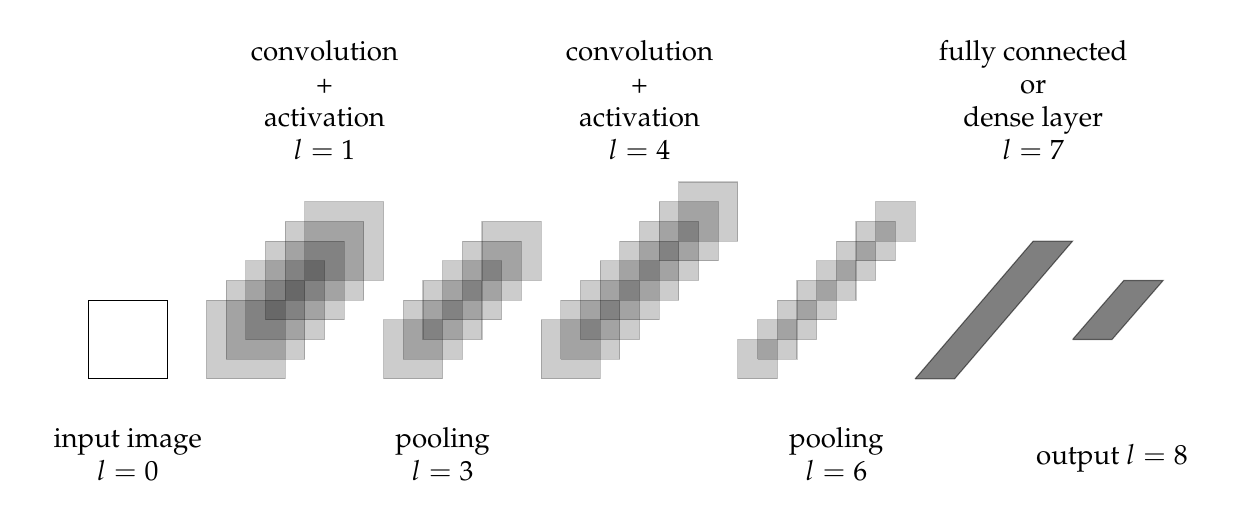
\begin{tikzpicture}
	\node at (0.5,-1){\begin{tabular}{c}input image\\ $l = 0$\end{tabular}};
	
	\draw (0,0) -- (1,0) -- (1,1) -- (0,1) -- (0,0);
	
	\node at (3,3.5){\begin{tabular}{c}convolution \\+\\ activation\\ $l = 1$\end{tabular}};
	
	\draw[fill=black,opacity=0.2,draw=black] (2.75,1.25) -- (3.75,1.25) -- (3.75,2.25) -- (2.75,2.25) -- (2.75,1.25);
	\draw[fill=black,opacity=0.2,draw=black] (2.5,1) -- (3.5,1) -- (3.5,2) -- (2.5,2) -- (2.5,1);
	\draw[fill=black,opacity=0.2,draw=black] (2.25,0.75) -- (3.25,0.75) -- (3.25,1.75) -- (2.25,1.75) -- (2.25,0.75);
	\draw[fill=black,opacity=0.2,draw=black] (2,0.5) -- (3,0.5) -- (3,1.5) -- (2,1.5) -- (2,0.5);
	\draw[fill=black,opacity=0.2,draw=black] (1.75,0.25) -- (2.75,0.25) -- (2.75,1.25) -- (1.75,1.25) -- (1.75,0.25);
	\draw[fill=black,opacity=0.2,draw=black] (1.5,0) -- (2.5,0) -- (2.5,1) -- (1.5,1) -- (1.5,0);
	
	\node at (4.5,-1){\begin{tabular}{c}pooling \\ $l = 3$\end{tabular}};
	
	\draw[fill=black,opacity=0.2,draw=black] (5,1.25) -- (5.75,1.25) -- (5.75,2) -- (5,2) -- (5,1.25);
	\draw[fill=black,opacity=0.2,draw=black] (4.75,1) -- (5.5,1) -- (5.5,1.75) -- (4.75,1.75) -- (4.75,1);
	\draw[fill=black,opacity=0.2,draw=black] (4.5,0.75) -- (5.25,0.75) -- (5.25,1.5) -- (4.5,1.5) -- (4.5,0.75);
	\draw[fill=black,opacity=0.2,draw=black] (4.25,0.5) -- (5,0.5) -- (5,1.25) -- (4.25,1.25) -- (4.25,0.5);
	\draw[fill=black,opacity=0.2,draw=black] (4,0.25) -- (4.75,0.25) -- (4.75,1) -- (4,1) -- (4,0.25);
	\draw[fill=black,opacity=0.2,draw=black] (3.75,0) -- (4.5,0) -- (4.5,0.75) -- (3.75,0.75) -- (3.75,0);
	
	\node at (7,3.5){\begin{tabular}{c}convolution \\+\\ activation\\ $l = 4$\end{tabular}};
	
	\draw[fill=black,opacity=0.2,draw=black] (7.5,1.75) -- (8.25,1.75) -- (8.25,2.5) -- (7.5,2.5) -- (7.5,1.75);
	\draw[fill=black,opacity=0.2,draw=black] (7.25,1.5) -- (8,1.5) -- (8,2.25) -- (7.25,2.25) -- (7.25,1.5);
	\draw[fill=black,opacity=0.2,draw=black] (7,1.25) -- (7.75,1.25) -- (7.75,2) -- (7,2) -- (7,1.25);
	\draw[fill=black,opacity=0.2,draw=black] (6.75,1) -- (7.5,1) -- (7.5,1.75) -- (6.75,1.75) -- (6.75,1);
	\draw[fill=black,opacity=0.2,draw=black] (6.5,0.75) -- (7.25,0.75) -- (7.25,1.5) -- (6.5,1.5) -- (6.5,0.75);
	\draw[fill=black,opacity=0.2,draw=black] (6.25,0.5) -- (7,0.5) -- (7,1.25) -- (6.25,1.25) -- (6.25,0.5);
	\draw[fill=black,opacity=0.2,draw=black] (6,0.25) -- (6.75,0.25) -- (6.75,1) -- (6,1) -- (6,0.25);
	\draw[fill=black,opacity=0.2,draw=black] (5.75,0) -- (6.5,0) -- (6.5,0.75) -- (5.75,0.75) -- (5.75,0);
	
	\node at (9.5,-1){\begin{tabular}{c}pooling\\ $l = 6$\end{tabular}};
	
	\draw[fill=black,opacity=0.2,draw=black] (10,1.75) -- (10.5,1.75) -- (10.5,2.25) -- (10,2.25) -- (10,1.75);
	\draw[fill=black,opacity=0.2,draw=black] (9.75,1.5) -- (10.25,1.5) -- (10.25,2) -- (9.75,2) -- (9.75,1.5);
	\draw[fill=black,opacity=0.2,draw=black] (9.5,1.25) -- (10,1.25) -- (10,1.75) -- (9.5,1.75) -- (9.5,1.25);
	\draw[fill=black,opacity=0.2,draw=black] (9.25,1) -- (9.75,1) -- (9.75,1.5) -- (9.25,1.5) -- (9.25,1);
	\draw[fill=black,opacity=0.2,draw=black] (9,0.75) -- (9.5,0.75) -- (9.5,1.25) -- (9,1.25) -- (9,0.75);
	\draw[fill=black,opacity=0.2,draw=black] (8.75,0.5) -- (9.25,0.5) -- (9.25,1) -- (8.75,1) -- (8.75,0.5);
	\draw[fill=black,opacity=0.2,draw=black] (8.5,0.25) -- (9,0.25) -- (9,0.75) -- (8.5,0.75) -- (8.5,0.25);
	\draw[fill=black,opacity=0.2,draw=black] (8.25,0) -- (8.75,0) -- (8.75,0.5) -- (8.25,0.5) -- (8.25,0);
	
	\node at (12,3.5){\begin{tabular}{c}fully connected\\ or\\ dense layer\\$l = 7$\end{tabular}};
	
	\draw[fill=black,draw=black,opacity=0.5] (10.5,0) -- (11,0) -- (12.5,1.75) -- (12,1.75) -- (10.5,0);
	
	\node at (13,-1){\begin{tabular}{c}output $l = 8$\end{tabular}};
	
	\draw[fill=black,draw=black,opacity=0.5] (12.5,0.5) -- (13,0.5) -- (13.65,1.25) -- (13.15,1.25) -- (12.5,0.5);
	\end{tikzpicture}
	\caption{Architecture of a typical \ac{CNN}. This representation was first proposed by \cite{lecun1995convolutional}.}
	\label{fig:trad_cnn}
\end{figure}

\subsection{Neural Networks for Image Reconstruction}

Image to image translation tasks require the \ac{CNN} to map from image in one domain to an image in another related domain. This requires the design of the \ac{CNN} to be quite different from the one depicted in Fig~\ref{fig:trad_cnn}. Convolution and pooling operations compress the input to obtain an abstract representation in lower dimensions. To transform the output into an image from the lower dimensional representation, transposed convolution operators are used. In contrast to the compressing nature of convolutions, they expand the input feature map. The combination of convolution+pooling and transposed convolutions are adjusted depending on the dimensions of the input and output images. Transposed convolution is shown in Fig~\ref{fig:tc}. Essentially the transposed convolution spatially reverses the dimensions of the convolution+pooling operation. 

\begin{figure}[!htbp]
	\centering
	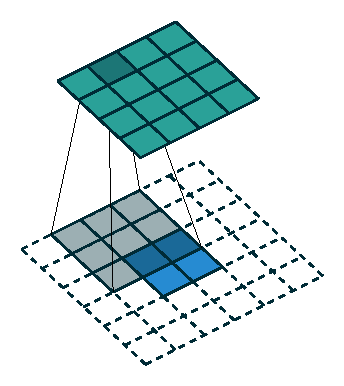
\includegraphics[width=0.5\linewidth]{transposed.pdf}
	\caption{Transposed convolution over a $2\times2$ input to get a $4\times4$ output. (\cite{dumoulin2016guide})}
	\label{fig:tc}
\end{figure}

Transposed convolutions are used in many tasks like super resolution, image segmentation, denoising and image reconstruction. This version of \ac{CNN} appropriate for image reconstruction is represented in Fig~\ref{fig:fcn}

\begin{figure}[!htbp]
	\centering
	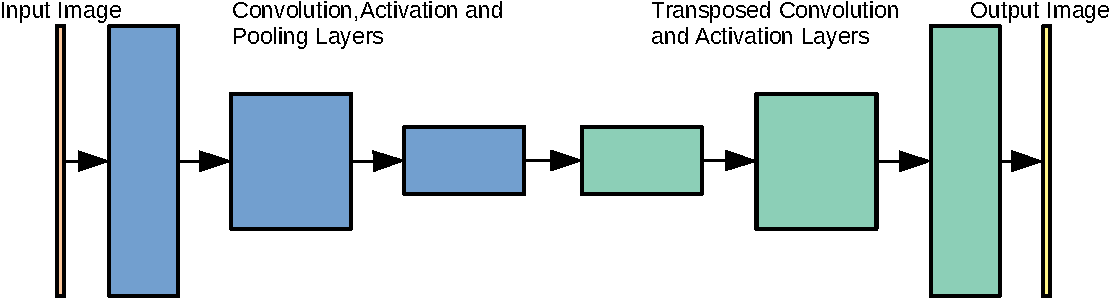
\includegraphics[width=1.0\linewidth]{fcn-crop.pdf}
	\caption{\ac{CNN} for image to image translation tasks. This example has an identical structure in convolution path and the transposed convolution path.}
	\label{fig:fcn}
\end{figure}

These architectures are sometimes referred to as \ac{CED}, since they contain two distinct paths of down sampling of input and up sampling of lower dimensional representation. The building blocks described in this section essentially form the basis of \ac{CNN}s proposed in this thesis. The next chapter consists of a review of existing works in deep learning applied to medical image reconstruction. And the following chapters describe the proposed methods. 



 
% Chapter 1

\chapter{Deep Learning and Tomographic Image Reconstruction} % Main chapter title

\label{Chapter3} % For referencing the chapter elsewhere, use \ref{Chapter1} 

%----------------------------------------------------------------------------------------
The impact of deep learning has been immense over the last few years in the field of medical imaging (\cite{litjens2017survey, greenspan2016guest}). Medical image reconstruction has also benefited hugely from the various advances in neural network architectures (\cite{wang2020deep,yedder2021deep,reader2020deep}). In the specific case of \ac{CT} image reconstruction, there has been active interest in sparse-view and low-dose reconstruction scenarios. While with \ac{PET} reconstruction on the other hand, low-dose imaging and total body imaging have been on the forefront. In both cases, obtaining high quality reconstructed images is a challenging task. Many established model-based iterative methods account for the low-dose and sparse-view settings to remove artifacts and noise from the reconstruction (\cite{nuyts1998iterative,Elbakri2002,liu2013total}). However, these methods require the knowledge of noise and artifacts statistics and generally have longer reconstruction times. Deep learning-based methods on the other hand are claimed to achieve reconstructed images with quality on par with iterative techniques and in a much shorter time frame (\cite{leuschner2021quantitative}). In this work, the focus has been on \ac{PET} and \ac{CT} image reconstruction. 
Image reconstruction corresponds to the task of mapping raw projection data retrieved from the detector to image domain. As depicted in Fig~\ref{fig:dl}, one can broadly identify three different categories of approaches for the implementation of deep learning within the framework of medical image reconstruction:
\begin{itemize}
	\item[(i)] methods that use deep learning as an image processing step that improves the quality of the raw data and/or the reconstructed image (\cite{gong2018pet, maier2018deep}); 
	\item[(ii)] methods that embed deep-learning image processing techniques in the iterative reconstruction framework to accelerate convergence or to improve image quality (\cite{xie2019generative,kim2018penalized,gong2019iterative});
	\item[(iii)] direct reconstruction with deep learning alone without any use of traditional reconstruction methods  (\cite{whiteley2019direct,zhu2018image,haeggstroem2018deeprec}).
\end{itemize}

\begin{figure}[!htbp]
	\centering
	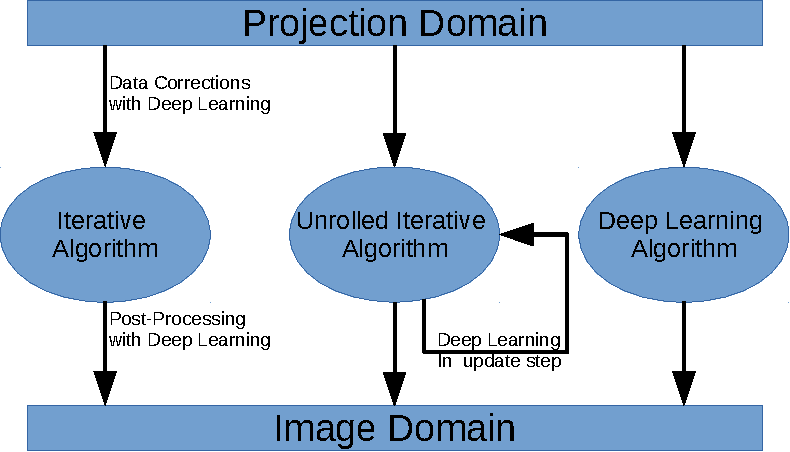
\includegraphics[width=0.8\linewidth]{./Figures/dl_mi.pdf}
	\caption{Deep Learning in Medical Image Reconstruction}
	\label{fig:dl}
\end{figure}


Each of these categories are discussed along with reference to some of the popular deep learning-based methods for \ac{CT} and \ac{PET} image reconstruction in this chapter. 

\section{Data Corrections or Post-processing}

The use of deep learning for the development of either data corrections or post-reconstruction  image based approaches has shown potential to improve the quality of reconstructed images. While it is possible to train a \ac{CNN} to regress directly from the measurement (raw data) domain to the image domain, the use of \ac{CNN} entirely in one particular domain makes it fast and relatively easy to implement. The motivation behind using deep learning architectures for these processing tasks is the extremely well documented performance in denoising and super resolution domains (\cite{tian2020deep,wang2020deep}). Data corrections involve improving the measurement data either through denoising or finding missing projection angle data. Post-processing in the image domain on the other hand consists of improving images reconstructed with standard reconstruction methods. 

Corrections in measured data $\boldy$ can be expressed as finding an estimate $\boldyhat$ through a neural network $F$ with parameters $\bm{\theta}$. 
\begin{equation}\label{eq:data_cor}
	\boldyhat = F_{\bm{\theta}} (\boldy)
\end{equation} 
The new set of corrected data $\boldyhat$ are then used to reconstruct images through traditional methods. An example of data corrections in \ac{PET} image reconstruction through sinogram repair is proposed by \cite{whiteley2019cnn}, where a \ac{CNN} is utilized to predict missing projection data for total body \ac{PET} image reconstruction. The repaired sinograms eventually improve image reconstruction by standard methods.

In \ac{CT} imaging, missing projection data in sparse-view setting is estimated through neural networks. An example in this regard is proposed in \cite{lee2018deep}, where the authors use U-Net to map sparse-view sinograms to full-view sinograms and then reconstruct the images using \ac{FBP}. Another idea to improve the raw data through scatter correction is proposed in \cite{maier2018deep}. In this work a modified U-Net is used to estimate scatter and correct the raw data in order to improve \ac{CT} images. 

Improvements in the images reconstructed by traditional methods are usually brought about through neural networks designed for denoising or super resolution. An image $\boldxhat$ ($\boldlambdahat$ or $\boldmuhat$) estimated by conventional methods like \ac{FBP} or \ac{OSEM} is improved through a neural network:

\begin{equation}\label{eq:post_pro}
\boldx_{\mathrm{den}} = \bm{F}_{\bm{\theta}} (\boldxhat)
\end{equation} 
where $\boldx_{\mathrm{den}}$ is the post-processed image. Over the years the trend in \ac{PET} imaging has been towards reducing the dose of the radiotracer injected into the patient, which in turn leads to noisier reconstructed images. The approach has been to create datasets with conventional algorithms (like \ac{OSEM}) for both low-dose and normal dose settings and then train a neural network to achieve normal dose quality starting from low-dose images. Apart from the low dose noise problem, in \ac{CT}, improvements in sparse-view imaging through deep learning has been an active area of research. The focus here is to reduce the artifacts produced by \ac{FBP} with sparse-view sinograms. These artifacts are either removed by first finding the missing projections and repairing the sinograms or by post-processing the images. In both these scenarios \ac{FBP} is utilized; in the former case neural network corrects the sinograms thereby providing full-view sinograms for reconstruction and in the latter case \ac{FBP} estimated artifact effected images are improved by the neural network.  

Some of the recent developments in post-processing and data corrections for \ac{PET} and \ac{CT} are summarized in Table~\ref{table:pp_PET} and Table~\ref{table:pp_CT}. A short description of the method along with the citation is given in the second column of both the tables. These approaches typically modify an existing neural network architecture to suit the problem they are addressing. U-Net is one of the most utilized architectures as seen in the third column where the base neural network is given. The datasets utilized by each of these works are mentioned in the final column. Along with the proposed modifications of established neural networks, these approaches typically use loss functions consisting of multiple components. The authors in \cite{gong2018pet} used perceptual loss along with \ac{MSE} to preserve qualitative and quantitative accuracy of the reconstructed images. The work proposed by \cite{whiteley2020fastpet} uses \ac{MSSIM} along with perceptual loss and \ac{MAE}. Another strategy used is pre-training on simulated data followed by fine-tuning on real patient data. Data corrections in the form of scatter correction of the sinogram data is proposed in \cite{qian2017deep}. The authors use \ac{CNN} followed by \ac{FC} layers in their approach. In \ac{CT} imaging there are works that do denoising of low-dose sinograms (\cite{ma2021sinogram,zhu2020low}) and also finding the missing projections in sparse-view sinograms (\cite{lee2018deep}). The same problem is tackled in the image domain through denoising (\cite{yang2018low}) and artifact removal for sparse-view problem (\cite{jin2017deep,xie2018artifact,zhang2018sparse}).
\begin{table}[ht!]
	\centering
	\caption{Summary of recent works on data corrections and post-processing approaches in \ac{PET}}
	\label{table:pp_PET}
	\scriptsize
	\begin{tabular}{||c|c|c|c||} 
		\hline
		Sl.No.    & Method             & Base Neural  & Dataset        \\ %[0.5ex] 
		          &                    &  Network     &                \\
		\hline\hline
		1         & \cite{gong2018pet} & \ac{CNN} with residual & BrainWeb and XCAT  \\     
		          &  Low-dose Image    &  blocks                & phantoms; Fine-tuning/testing  \\ 
		          &   Denoising        & & with real patient data       \\ 
		\hline
		2         &  \cite{whiteley2020fastpet}& U-Net with residual & Real PET/CT data \\
		          & Histo Image        & blocks      &        \\
		          & Correction         &                &        \\
		\hline  
		3         & \cite{zhao2020study}& Cycle GAN    & Real PET/CT data  \\ 
       	          & Low-dose Image      &              &                   \\ 
       	          & Denoising           &              &                   \\ 
       	\hline
       	4         & \cite{qian2017deep} & CNN with fully    & Monte Carlo simulations  \\ 
                  & Sinogram Scatter    & connected layer   & with phantoms            \\ 
       	          & Correction          &                   &                          \\ 
       	\hline
       	5         & \cite{hong2018enhancing}& Deep residual CNN & Digital phantoms  \\ 
       	          & Single Image Super      &                   &             \\ 
       	          & Resolution for sinograms&                   &                          \\ 
       	\hline
       	6         & \cite{sanaat2021deeptofsino}&   ResNet       & Real TOF-PET/CT data  \\ 
       	          & Low-dose to full-dose    &                   &             \\ 
       	          & sinogram synthesis    &                      &                          \\ 
       	\hline
       	
	\end{tabular}
	
\end{table}

\begin{table}[ht!]
	\centering
	\caption{Summary of recent works on data corrections and post-processing approaches in \ac{CT}}
	\label{table:pp_CT}
	%\footnotesize
	\scriptsize
	\begin{tabular}{||c|c|c|c||} 
		\hline
		Sl.No.    &       Method             & Base Neural          & Dataset        \\ %[0.5ex] 
            	  &                          &    Network                      &                \\
		\hline\hline
		1         & \cite{lee2018deep}       &   Residual U-Net     & Simulated projections          \\     
		          &  Sinogram synthesis      &                      & from real patient data         \\ 
		          &   for sparse-view CT     &                      &                                \\ 
		\hline
		2         &  \cite{jin2017deep}      & Residual U-Net       & Phantom and Real patient       \\
		          & Artifact removal in      &                      &   data along with projections  \\
		          & sparse-view reconstructed images&               &                                \\
		\hline  
		3         & \cite{xie2018artifact}   & Improved GoogleNet   & Simulated projections          \\ 
		          & Artifact removal in      &                      & from real data                 \\ 
		          & sparse-view reconstructed images&               &                                \\ 
		\hline
		4         & \cite{zhang2018sparse}    & DeneNet with        & Simulated projections          \\ 
		          & Artifact removal in       & deconvolutions      & from real data                 \\ 
		          & sparse-view reconstructed images&               &                                \\ 
		\hline
		5         & \cite{ma2021sinogram}     & Attention residual  & Real data along with           \\ 
		          & Low dose sinogram         &  dense CNN          & projections                    \\ 
		          & denoising                 &                     &                                \\ 
		\hline
		6         & \cite{yang2018low}        &    Wasserstein-GAN & Real data along with            \\ 
		          & Low-dose image            &                    & projections                     \\ 
		          & denosing                  &                    &                                 \\ 
		\hline
		7         & \cite{zhu2020low}         &  Three-segment network  & Real data along with            \\ 
		          & Simultaneous sinogram and &  ADAPTIVE-NET      & projections                     \\ 
	 	          & image domain denoising    &                    &                                 \\ 
		\hline
		
	\end{tabular}
	
\end{table}

An important aspect of the methods discussed in this section is that they all claim to provide fast reconstructed images using well established neural network architectures. This also stems from the fact that most of these approaches start with an image estimate that is also obtained with a relatively faster conventional method, like \ac{FBP} for \ac{CT} and \ac{OSEM} for \ac{PET}. These fast estimates are usually very noisy or artifact ridden. These approaches rely on the neural network to handle the noise and artifacts. The attractiveness of these methods is the simplicity, ease of implementation and the lack of requirement of large datasets. 

\section{Hybrid Methods}

The methods mentioned in this section and the next, are directly involved in the reconstruction process, rather than being exclusive to data corrections or post-reconstruction processing. The hybrid methodology for image reconstruction combines model-based and neural network approaches exploring the benefits of both methods. In this section we discuss some of the recent works in both \ac{PET} and \ac{CT} that fall in the category of hybrid methods.

\begin{itemize}


\item Data-driven information learned by a neural network can be incorporated into an iterative algorithm through the regularization term. \cite{gong2019iterative} used a modified version of the U-Net comprising of multi-channel input to represent \ac{PET} images.
\begin{equation}\label{eq:iter_CNN}
\boldlambda = F_{\bm{\theta_{\mathrm{fixed}}}}(\bm{z})
\end{equation} 
where $F_{\bm{\theta_{\mathrm{fixed}}}}$ represents the trained denoising neural network (modified U-Net) with fixed trainable parameters $\bm{\theta_{\mathrm{fixed}}}$ and $\bm{z}$ represents the input to the neural network. The \ac{PET} reconstruction model (from \ref{eq:PET}) can be modified to incorporate \ref{eq:iter_CNN}. 

\begin{equation}\label{eq:mod_PET}
	\boldybar(\boldlambda) = \boldA F_{\bm{\theta_{\mathrm{fixed}}}}(\bm{z}) + \bm{r}
\end{equation}
The unknown image $\boldlambda$ can be estimated using the maximum likelihood criterion:
\begin{equation}\label{eq:iter_CNN2}
\boldlambdahat = F_{\bm{\theta_{\mathrm{fixed}}}}(\bm{\hat{z}})
\end{equation} 
\begin{equation}
\boldlambdahat=\underset{\boldlambda \ge 0}{\operatorname{argmin}} \; L(\bm{z})
\end{equation}

In order to ease the difficulty of solving the above due to the non-linearity of the neural network, the authors adapted a constrained version of the above:

\begin{equation}\label{constr}
 	\operatorname{max} \; L(\bm{\boldlambda});  \; \mathrm{s.t.} \; \boldlambda = \bm{F}_{\bm{\theta_{\mathrm{fixed}}}}(\bm{\hat{z}})
\end{equation}
To solve the above optimization problem the authors used the augmented Lagrangian format:
\begin{equation}
L_{\rho}=L(\boldlambda)-\frac{\rho}{2}\|\boldlambda-\bm{F}_{\bm{\theta_{\mathrm{fixed}}}}(\bm{z})+\bm{\gamma}\|^{2}+\frac{\rho}{2}\|\bm{\gamma}\|^{2},
\end{equation}
The authors used the \ac{ADMM} algorithm to split the above into three steps:

\begin{equation}\label{eq:ad1}
\boldlambda^{N+1}=\underset{\boldlambda}{\arg \max} \; L(\boldlambda)-\frac{\rho}{2}\left\|\boldlambda-\bm{F}_{\bm{\theta_{\mathrm{fixed}}}}(\bm{z})^{N}+\bm{\gamma}^{N}\right\|^{2}
\end{equation}

\begin{equation}\label{eq:ad2}
\bm{z}^{N+1}=\arg \min \left\|\bm{F}_{\bm{\theta_{\mathrm{fixed}}}}(\bm{z})-\left(\boldlambda^{N+1}+\bm{\gamma}^{N}\right)\right\|^{2}
\end{equation}

\begin{equation}\label{eq:ad3}
\bm{\gamma}^{N+1}=\bm{\gamma}^{N}+\boldlambda^{N+1}-\bm{F}_{\bm{\theta_{\mathrm{fixed}}}}(\bm{z})^{N+1}
\end{equation}
\ref{eq:ad1} is equivalent to penalized \ac{PET} reconstruction and the authors used the optimization transfer method proposed in \cite{wang2012penalized}. The second part of the algorithm (from \ref{eq:ad2}) involving the input $\bm{z}$ update, is a non-linear version of the least squares problem. In the above methodology, the network parameters $\bm{\theta}$ are fixed while the input to the network $\bm{z}$ is updated. The authors extended this approach in \cite{gong2018pet2} by using a fixed input to the network $\bm{z}_{\mathrm{fixed}}$, while setting the network parameters to update. The fixed input to the network was an MRI image while the network training was based on the concept of deep image prior (\cite{ulyanov2018deep}). The second sub-problem was modified to reflect the update in the network parameters:

\begin{equation}\label{eq:dip}
\bm{\theta}^{N+1}=\arg \min \left\|\bm{F}_{\bm{\theta}}(\bm{z_{fixed}})-\left(\boldlambda^{N+1}+\bm{\gamma}^{N}\right)\right\|^{2}
\end{equation}

Both these methods require that the raw data also agree with the denoising \ac{CNN}. The images reconstructed are reported to have better lesion contrast compared to the post-processing \ac{CNN} denoising approaches, indicating an advantage of the hybrid methods, despite being slightly tedious to implement and having longer prediction times.

\item Apart from using neural networks for regularization, the prior information captured by them can be combined with established model-based methods. One such approach called FBSEM-Net was proposed by \cite{mehranian2020model}. Their unrolled method is based on forward-backward splitting (FBS) algorithm. The objective function for their method was:

\begin{equation}
\boldlambda^{N}=\underset{\boldlambda}{\operatorname{argmax}}\left\{L(\boldlambda \mid \boldy)-\frac{1}{2 \beta}\left\|\boldlambda-\boldlambda_{R e g}^{N}\right\|^{2}\right\}
\end{equation}
with $\beta$ being a hyper-parameter that controls the balance between the data fidelity term and the regularization term. The authors solved the above through the method of separable surrogates proposed in \cite{depierro1995}. The three steps involved in obtaining the final image update: computing the regularization term, finding the EM update and fusing the EM update with the neural network estimated prior. The first step to compute the regularization term can be written as:

\begin{equation}\label{eq:fbs1}
\boldlambda_{reg}^N = F(\boldlambda^{N-1})
\end{equation} 
where $F$ is a residual neural network estimating the regularization term based on the image from the previous iteration. 
The second step involved getting the EM update $\boldlambda_{EM}^{N}$ similar to \ref{eq:mlem}. Finally the image is estimated by
\begin{equation}\label{eq:fb2}
\begin{array}{l}
\lambda_j^{N+1} 
=\frac{2 \lambda_{E M}^{N}}{\left(1-\delta_{j} \lambda_{j, R e g}^{N}\right)+\sqrt{\left(1-\delta_{j} \lambda_{j, R e g}^{n}\right)^{2}+4 \delta_{j} \lambda_{j, E M}^{n}}} ,\; \delta_{j}=\frac{1}{\beta s_{j}}
\end{array}
\end{equation}

During the network training, two reconstructions occur simultaneously, one with good quality reference data and the other with noisy data. The role of the neural network is to denoise the current estimate, such that the fused combined image using \ref{eq:fb2} best agrees with the high quality \ac{MLEM} reconstructed image. The overall methodology constitutes of a very deep network with each iteration being a block of \ac{CNN} along with the conventional \ac{MLEM} layers. 


\item \cite{adler2018learned} proposed a learned primal-dual algorithm which was one of the first methods that combined \ac{MBIR} methods with deep learning for low-dose \ac{CT} image reconstruction. The authors proposed a generalized algorithm that could be modified for other tomographic imaging modalities also. \acp{CNN} are used both in the image domain and the sinogram domain, connected through the forward projection operator and it's adjoint. In many \ac{MBIR} approaches, non-smooth regularizers are used. They are typically handled through smooth approximations which lead to additional parameters and non-exact solutions. As an alternative, proximal methods are used to tackle the non-smooth objective functions. The method proposed in this article was inspired from one such proximal \ac{PDHG} algorithm (\cite{chambolle2011first}). They replaced the proximal operators with learned parameterized operators (\acp{CNN}) to result in a learned reconstruction operator. The primal and dual operators were parameterized as \acp{CNN} consisting of 3 layers and in total of 64 intermediate convolution channels. The different steps involved in the method are summarized in Algorithm~\ref{alg:pd}. The neural networks and the projection/back-projection operators were implemented using operator discretization library (ODL) and Tensorflow (\cite{abadi2016tensorflow}). The authors tested their approach on ellipse phantoms and real patient data. They reported better qualitative and quantitative results when compared to TV and deep learning-based post-processing method. 

\begin{algorithm}
\SetAlgoLined
For primal and dual variables $x \in X^{N_{primal}}$ and $h \in X^{N_{dual}}$, proximal dual and primal operators represented by neural networks,  $\Gamma_{\theta_{k}^{d}}$, $\Lambda_{\theta_{k}^{p}}$, K iterations, measurement data $\boldy$ \\
\For{k = 1,2,\dots, K}{
	$\bm{h}^{[k]}=\Gamma_{\theta_{k}^{d}}\left(\bm{h}^{[k-1]}, \bm{A}\left(\boldx_{(2)}^{[k-1]}\right), \boldy\right)$
		
	$\boldx^{[k]}=\Lambda_{\theta_{k}^{p}}\left(\boldx^{[k-1]},\left[\bm{A}\left(\boldx_{(1)}^{[k-1]}\right)\right]^{*}\left(\bm{h}_{(1)}^{[m]}\right)\right)$
				
	}
\Return $\boldxhat = \boldx_{(1)}^{[K]}$
\caption{Learned Primal-Dual}
\label{alg:pd}
\end{algorithm}


\item A hybrid method for sparse-view \ac{CT} was proposed in \cite{wu2021drone}. The authors propose a three-stage reconstruction framework consisting of embedding, refinement and awareness. The first module extends the sinogram and reduces the sparse-view artifacts. The refinement part of the method recovers finer details in the images and finally the last module regularizes the images from the earlier modules by ensuring consistency between the measurement data and images. The last module was adapted from compressed sensing and it ensures stability and generalizability in the reconstructed images. The embedding module consists of two neural networks $F_1$ and $F_2$, the first one is a U-Net that operates in the sinogram domain, mapping from 60 views to 180 views, and the second one a W-GAN that operates in the image domain refining the image obtained through \ac{FBP} on the upsampled sinograms. It can be represented as follows:

\begin{equation}
\boldx^{\prime}=F_{2}(\bm{A_{2}}^{+}(F_{1} (\boldy)))
\end{equation}
where $\boldx^{\prime}$ is the image estimated by the embedding module, $\bm{A_2}^{+}$ is the \ac{FBP} reconstruction operator for the up-sampled views ($180$). The next module maintains a balance between the extension of views and refining the subsequent details in the images through two neural networks similar to the ones in the first module. The residual between the image predicted by the embedding module and the re-sampled sinogram can be written as: $(\boldy'-\boldA_{2} \boldx')$. The first neural network is trained to minimize the \ac{MSE} between the measurement data labels and predictions.   

\begin{equation}
	\boldy'' = F_3(\boldy'-\boldA_{2} \boldx')
\end{equation} 
The second neural network in the refinement module is trained to minimize the \ac{MSE} between the image data and labels resulting in a refined image:

\begin{equation}
\boldx'' = F_4(\boldA_{2}^{+}(\boldy''))
\end{equation} 
The measurement data and the images are then updated with the predictions from the trained networks:

\begin{equation}
	\boldy^d = \boldy'' + \bm{A_{2}} \boldx' 
\end{equation}

\begin{equation}
    \boldx^d = \boldx' + \boldx''
\end{equation}


The final module combines the deep learning-based data image priors ${\boldy^d,\boldx^d}$ and the compressed sensing framework to arrive at an objective function as follows:

\begin{equation}\label{eq:cs}
\min _{\boldx}\left\{\begin{array}{l}
\frac{1}{2}\left\|\mathbf{y}-\mathbf{A}_{1} \boldx \right\|^{2}+\frac{\alpha_{1}}{2}\left\|\boldy^{d}-\mathbf{A}_{2} \boldx\right\|^{2} \\
+\frac{\alpha_{2}}{2} \mathrm{~W} \boldx+\frac{\alpha_{3}}{2} \mathrm{~W}\left(\boldx-\boldx^{d}\right)
\end{array}\right\}
\end{equation}
where $\alpha_{1} \ge 0$ balances the two data fidelity terms, $\boldA_{1}$ represents the system matrix that projects the lower-sampled data (60 views) and $\boldA_{2}$ represents the system matrix that projects the higher up-sampled data (180 views). For the regularization the authors used a variation of TV, called total difference represented by $W$. $\alpha_{2}$ and $\alpha_{3}$ are the regularization hyper-parameters. The authors validated their method on clinical and pre-clinical datasets and reported superior performance of their proposed method when compared to deep learning-based methods like FBPConvNet (\cite{jin2017deep}), HD-Net (\cite{wu2020high}) and DL-PICCS (\cite{zhang2020deep}).

\end{itemize}
 
Other works in the hybrid approach include the article by \cite{xie2019generative}, who extended the method proposed by \cite{gong2019iterative} by replacing the U-Net with a \ac{GAN} for image representation within the iterative framework. \cite{kim2018penalized} incorporated a trained denoising convolutional neural network (DnCNN) along with a novel local linear fitting function into the iterative algorithm. The DnCNN which is trained on data with multiple noise levels improves the image estimate at each iteration. They used simulated and real patient data in their study. In \cite{gupta2018cnn}, a U-Net is used to encode the prior, i.e., to project the current estimate to the prior image set while gradient descent enforces measurement consistency. \cite{xiang2021fista} proposed a hybrid method named FISTA-Net which is a combination of the model-based \ac{FISTA} and neural network. The parameters of FISTA-Net like gradient step size, threshold and momentum scalar are learned from the data rather than through fine-tuning. FISTA-Net was demonstrated to be effective for multiple imaging modalities including \ac{CT}. The drawbacks of the methods described in this section are the slow reconstruction time and high computational expense, since the optimization procedure is carried out also during test time. Despite the advantage of producing state of the art results (\cite{reader2020deep,leuschner2021quantitative}) along with the stability and consistency offered by these hybrid methods, the justification of complexity vs accuracy trade-off is still a topic of active research. 


\section{Direct Reconstruction with Deep Learning}

The third approach is using deep learning-based methods to directly map from projection to image space. Essentially neural network can be modeled to approximately learn the inverse mapping from measurement $\boldy$ to image $\boldx$. A neural network $F$ with trainable parameters $\bm{\theta}$ can be represented as:

\begin{equation}\label{eq:direct}
\boldxhat=F_{\bm{\theta}}(\boldy)
\end{equation}
where $\boldxhat$ is the reconstructed image estimated by the neural network. Once trained, the images are reconstructed from the sinograms by a single pass though the network, making it the fastest approach for image reconstruction. 

The deep learning architecture proposed by \cite{zhu2018image} called AUTOMAP uses \ac{FC} layers (which encode the raw data information) followed with convolutional layers. The first three layers in this architecture are \ac{FC} layers with dimensions $2n^2$, $n^2$ and $n^2$ respectively where $n\times{}n$ is the dimension of the input image. The AUTOMAP requires the estimation of a huge number of parameters which makes it computationally intensive. Although initially developed for \ac{MRI}, AUTOMAP has been claimed to work on other imaging modalities too. Brain images encoded into sensor-domain sampling strategies with varying levels of additive white Gaussian noise were reconstructed with AUTOMAP.  Within the same concept of using \ac{FC} layers' architectures a three stage image reconstruction pipeline called DirectPET has been proposed to reduce associated computational issues  \cite{whiteley2019direct}. The first stage down-samples the sinogram data, following which a unique Radon transform layer encodes the transformation from sinogram to image space. Finally the estimated image is improved using a super resolution block. This work was applied to full body \ac{PET} images and remains the only approach that can reconstruct multiple slices simultaneously (up to 16 images). DeepPET is another approach implemented on simulated images using \ac{CED} architecture based on the neural network proposed by the visual geometric group \cite{haeggstroem2018deeprec}. Using realistic simulated data, they demonstrated a network that could reconstruct images faster, and with an image quality (in terms of root mean squared error) comparable to that of conventional iterative reconstruction techniques. \cite{liu2019deep} proposed a direct conditional \ac{GAN} based approach, that replaced the \ac{CED} with a U-Net.    


For direct \ac{CT} image reconstruction, \cite{li2019learning} proposed an architecture termed iCT-Net consisting of $12$ layers that are a combination of convolutions and modified fully-connected layers. The $12$ layers are separated into segments and are trained separately before being combined for end-to-end training. To reduce the number of parameters in learning the mapping for full resolution \ac{CT} reconstruction, \cite{fu2019hierarchical} proposed a breakdown of the problem into smaller fragments that can be mapped onto a hierarchical network architecture. The approach proposed in \cite{ye2018deep} converts the sinogram data into a stack of back projections for each angle, which are then fed into a \ac{CNN}. The spatial in-variance of the \ac{CNN} is exploited to learn the mapping from these single view stacked back projections onto reconstructed images. Currently, we observe that adversarial networks are increasingly used in scenarios with high-resolution images. In \cite{thaler2018sparse} a W-GAN is proposed for sparse-view \ac{CT} image reconstruction. The authors used a combination of $L_1$ loss and adversarial loss to train their network. The generator in their work is a U-Net and the discriminator a typical classification \ac{CNN}. It is to be noted that the authors performed their experiments on down-sampled images of resolution $128\times 128$. The direct approach appears to exploit the power of neural networks to the fullest, however, the challenges include data management, large number of training parameters and stability at testing time. Among the three approaches discussed they have the least stability when tested with different configurations of data \cite{antun2020instabilities}. However, with the constant developments in neural network designs, the possibility of arriving at a network most suitable for image reconstruction cannot be ruled out.





% Chapter 4

\chapter{LRR-CED:  Low-Resolution Reconstruction aware Convolutional Encoder-Decoder Network  for Direct Sparse-View CT Image Reconstruction} % Main chapter title

\label{Chapter4} % For referencing the chapter elsewhere, use \ref{Chapter1} 

Sparse-view \ac{CT} reconstruction has been at the forefront of research in medical imaging. Reducing the total X-ray radiation dose to the patient while preserving the reconstruction accuracy is a big challenge. The sparse-view approach is based on reducing the number of rotation angles, which leads to poor quality reconstructed images as it introduces several artifacts. These artifacts are more clearly visible in traditional reconstruction methods like the \ac{FBP} algorithm. Over the years, several model-based iterative and more recently deep learning-based methods have been proposed to improve sparse-view \ac{CT} reconstruction. Many deep learning-based methods improve \ac{FBP}-reconstructed images as a post-processing step. In this work, we propose a direct deep learning-based reconstruction that exploits the information from low-dimensional \ac{FBP} estimates, to learn the  projection-to-image mapping. This is done by concatenating the \ac{FBP} estimate at multiple resolutions in the decoder part of a \ac{CED}. This approach is investigated on two different networks, based on Dense Blocks and U-Net to show that a direct mapping can be learned from a sinogram to an image.  The results are compared to a post-processing deep learning method and an iterative method that uses a \ac{TV} regularization. 


\section{Main Contribution}

The main drawbacks of current deep learning-based direct image reconstruction algorithms are the tedious training process necessary to train large networks with large number of trainable parameters and the requirement of high memory in case of high-resolution \ac{CT} images. 
In this work we propose a new method for direct deep learning based sparse-view \ac{CT} image reconstruction with fully convolutional networks. We use two networks, namely Fully Convolutional Densenets \cite{jegou2017one} and U-Net \cite{ronneberger2015u}. An important characteristic of both these architectures \cite{jegou2017one,ronneberger2015u} is the presence of concatenation from the encoding layers to the decoding layers that ensures the usage of features from the input for the reconstruction. Specifically, for application in sparse-\ac{CT} image reconstruction, the network would have sparse-view sinograms as input and reconstructed images as output. The original application in the medical imaging field of both these architectures was in image segmentation, where the image-to-image mapping operates in the same image domain. Medical image reconstruction on the other hand involves mapping between two different domains (sinogram to image). In order to help the network to learn the mapping from sinogram to image, we propose the use of \ac{FBP} image estimates of the sparse sinograms and concatenate them with the feature maps of the decoder. 

% \AP{Here the motivation for this "intuition" should be stated maybe you can introduce some simple notation already here: Given that we only have access to sparse measurement data (sinogram $\boldy$), we can enforce that the inverse mapping $f$ at each layer/ sub-resolution of the network is consistent in the measurement domain. That is 	$\boldL f(\boldy) = \boldy$.  this can be achieved by using concatenating as feature maps a (fast) low-resolution FBP for each or a subset of levels of the network. While this leads to a massive reduction of the parameters (number of layers) required in the network, the network parameters has to be trained accordingly since the above mentioned constraint is not enough to learn the inverse mapping, as it cannot capture information about the image $\boldx$ outside the range of the physical under-determined operator $\boldL$ (Radon transform for CT). Do not put details of the implementation in the introduction rather put the general idea behind.}

Given that we only have access to sparse measurement data, taking the form of a sinogram $\boldy$, we can enforce that the inverse mapping $\boldf$ at each layer/sub-resolution of the network is consistent in the measurement domain. That is $\boldP \boldf(\boldy) = \boldy$. This can be achieved by concatenating, as feature maps, (fast) low-resolution \ac{FBP}-reconstructed images for each or a subset of the network levels. While this leads to a massive reduction of the parameters (fully convolutional layers instead of fully-connected) required in the network, the above-mentioned constraint is not enough to learn the inverse mapping as it cannot capture information about the image $\boldx$ outside the range of the physical under-determined operator $\boldP$ (Radon transform for CT). Hence, the network needs to be trained accordingly.

Once the network is trained, these custom concatenations enable architectures that were previously used for denoising/artifact removal to learn a mapping from sparse sinograms to full-resolution \ac{CT} images. One characteristic feature of reconstructions generated by deep learning-based methods is the blurriness of the outputs. To counteract this we used perceptual loss involving features extracted from two different levels of $\mathrm{VGG16}$ network (Block 1 and Block 3). Since the exclusive use of perceptual loss results in unrealistic artifacts we couple it with a $L_1$ loss. A general representation of the proposed approach is depicted in Figure~\ref{fig:ge}. It consists of a \ac{CED} network with two blocks in both the encoder and the decoder that takes in as input a reshaped sparse sinogram which has the same dimensions as the output image. A concatenation of two resolutions $h_1 \times w_1$ and $h_2 \times w_2$ is incorporated in the decoder. 

The main contributions of our work are summarized as follows:
\begin{itemize}
	\item A new approach for sparse-view \ac{CT} image reconstruction using fully-convolutional networks
	\item Use of lower resolution \ac{FBP} estimates which enable the networks that are predominantly used for denoising to learn the more complex mapping from sinogram to image domain. 
	\item Two neural networks are implemented to test this approach using different levels of sparsity in the sinograms. 
\end{itemize}

\begin{figure}[!htbp]
	\centering
	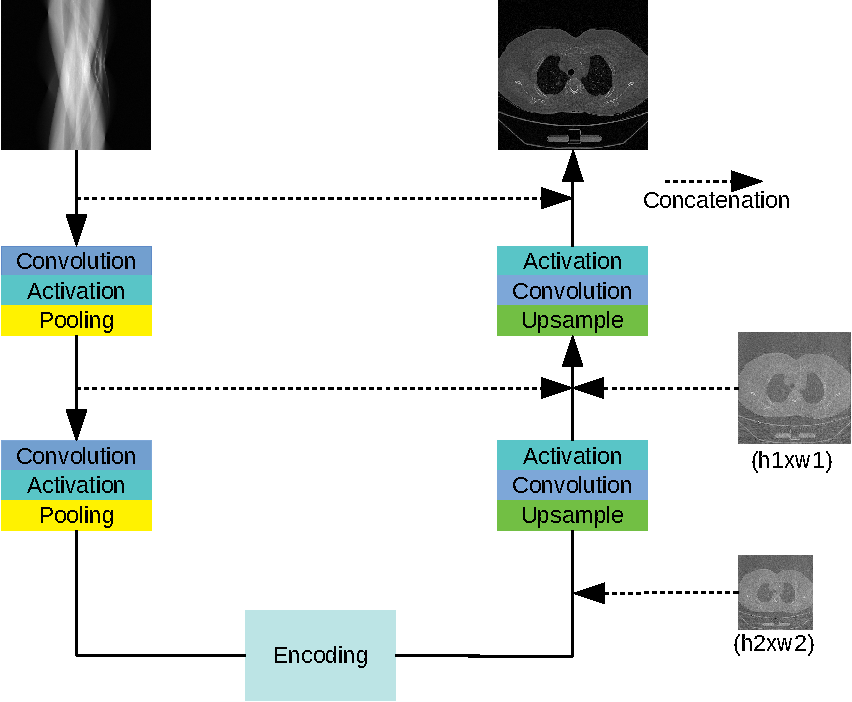
\includegraphics[width=0.7\linewidth]{general_enc-crop.pdf}
	\caption{General representation of an encoder-decoder architecture with fully convolutional layers and the proposed \ac{FBP} concatenations ($\boldx_1$ and $\boldx_2$) at two different resolutions $h_1 \times w_1$ and $h_2 \times w_2$}
	\label{fig:ge}
\end{figure}


\section{Methods}

\subsection{Proposed Low Resolution Reconstruction aware \ac{CED} Model}

Supervised deep learning-based methods learn the mapping between the measurement $\boldy$ and the corresponding reconstructed image $\boldx$. In the case of direct deep learning-based image reconstruction this mapping is typically learned via neural networks which can be represented as a function $\boldf_{\Theta}\colon \bbR^n \to \bbR^m$ with trainable parameters $\Theta$: 
\begin{equation}\label{eq:dl}
\boldxhat = \boldf_{\Theta}(\boldy) \, .
\end{equation}  
where, $\boldxhat$ is the predicted image. 

Most of the works in direct reconstruction for sparse-view \ac{CT} represent $\boldf$ with a neural network with fully-connected layers. These networks require huge memory and large datasets for training. As an alternative to this, we propose the use of fully convolutional encoder-decoder networks that have lesser trainable parameters and are faster to train. 
The main idea is to enforce data consistency by providing estimates at different resolutions $\boldxhat_r$, $r = 1, \ldots, R$:
\begin{equation}\label{eq:d}
\boldxhat = \boldf_{\Theta}(\boldy,   (\boldxhat_r)_{r=1}^R    ) 
\end{equation}  
where each $\boldxhat_r \in \bbR^{m_r}$, $m_r < m$, is an approximate solution of
\begin{equation}\label{eq:xr}
\boldy = \boldP \boldU_r \boldxhat_r
\end{equation} 
with $\boldU_r\in\bbR^{m\times m_r}$ being an upsampling operator.

In a typical \ac{CED}, the encoder learns the representation of the input domain and the decoder learns to map this representation to the corresponding image in the output domain. In the specific case of a \ac{CED} for medical image reconstruction, the encoder operates in the sinogram space and the decoder in the image space. Based on this hypothesis, we propose to concatenate the estimates at different levels of the decoder part of the network. The function of these concatenations is to help the network learn the structure of the image. The feature maps at different levels of the decoder have different resolutions. Hence, concatenating the estimate $\boldxhat_r$ at different levels requires the estimate to be of the appropriate resolution. The different convolutional layers in the decoder work towards arriving at a clear reconstructed image that is free of artifacts and noise. The estimate $\boldxhat_r$ is obtained with a sparse sinogram, hence it is artifact-ridden and noisy. Therefore, concatenating the estimate $\boldxhat_r$ at a level closer to the output resolution is counter productive as the network has lesser number of convolutional layers to correct the noise and artifacts. On the other hand the estimate at lower resolutions has lesser structural information compared to the estimates at higher resolution. The selection of $\boldxhat_r$ should ensure a balance between aiding the network to learn the structure of the image and enabling it to correct the artifacts and noise. 

Our method, namely \ac{LRRCED}, was implemented with $R=2$ and the image estimates $\boldxhat_r$ were obtained by \ac{FBP} at lower resolution. With the help of a series of experiments, we determined the best possible configuration for concatenating $\boldxhat_r$. In section Section~\ref{sec:concat}, we present quantitative evaluation of the effect of these concatenations on the reconstructed images. 

We investigate \ac{LRRCED} with two different variations for $\boldf$, \ac{LRRCED}(D) with Fully Convolutional DenseNets and \ac{LRRCED}(U) with U-Net, which are discussed in Section~\ref{sec:FCDN} and Section~\ref{sec:UNet}. 




\subsubsection{Fully Convolutional Dense Networks}\label{sec:FCDN}

A fully convolutional dense network was used as first variation of \ac{LRRCED}. Dense networks \cite{huang2017densely} are based on the hypothesis that connecting all the layers to each other in a feed forward fashion leads to higher accuracy and easier training of the network. A typical dense block of three layers is depicted in Figure~\ref{fig:db}. The extension of dense networks for image segmentation was proposed by \cite{jegou2017one}. The three  blocks involved in the construction of this network are \ac{DB} with $l$ number of layers, \ac{TU} and \ac{TD}. The combination of these three blocks helps in building an encoder-decoder structure suitable for tasks dealing with image-to-image domain transfer. Each layer consists of batch normalization, \ac{ReLU} activation and $3\times 3$ convolution. \ac{TD} includes: batch normalization, \ac{ReLU}, $1\times 1$ Convolution and $2\times 2$ max pooling. Finally, \ac{TU}  includes a $3\times 3$ transposed convolution with stride $2$. The important modification to the architecture blocks in our work is the removal of the dropout layers. The fully convolutional dense network with proposed concatenations is represented in Figure~\ref{fig:dn}. For the sake of representation we included only $5$ dense blocks in the figure. The complete architecture details are given in Table~\ref{table:1a}. 


\subsubsection{U-Net}\label{sec:UNet}

One of the most established architectures for image-to-image translation is U-Net \cite{ronneberger2015u}, which we used as second variation of \ac{LRRCED} (called from here on-wards as \ac{LRRCED}(U)).
 
A typical U-Net consists of Convolution, Activation (\ac{ReLU}) and Pooling layers in the encoder and Upsampling, Convolution and Activation in the decoder. We have used U-Net without the dropout, similar to the dense network. The U-Net is represented in Figure~\ref{fig:un}. 

\begin{figure}[!htbp]
	\centering
	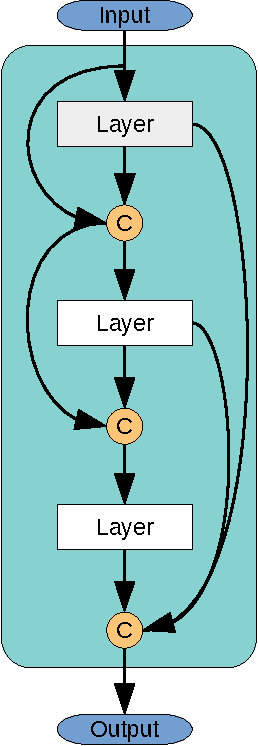
\includegraphics[width=0.23\linewidth]{./Figures/dense_block-crop.pdf}
	\caption{Representation of a Dense Block with three layers.}
	\label{fig:db}
\end{figure}



\begin{figure}[!t]
	\centering
	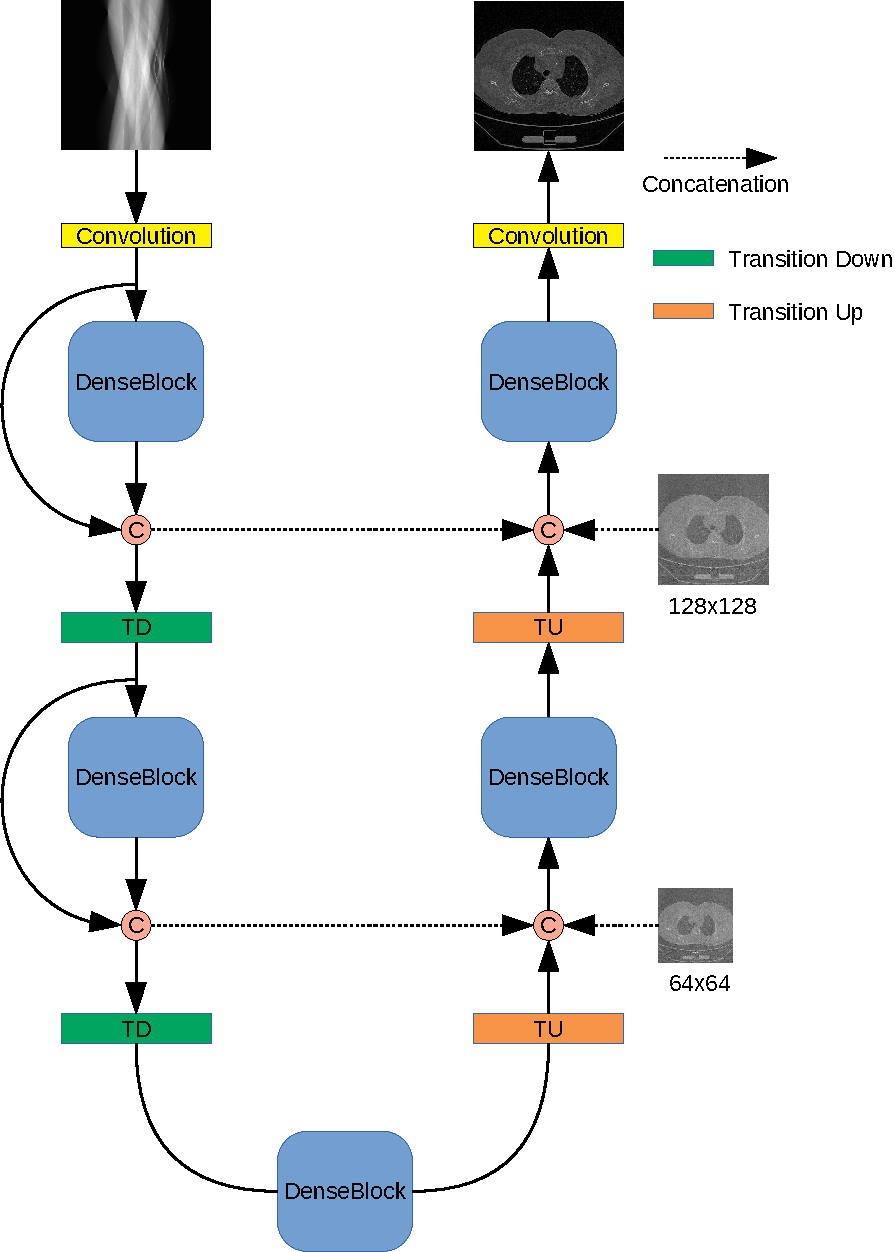
\includegraphics[width=.83\linewidth]{./Figures/densenet-crop.pdf}
	\caption{\ac{LRRCED}(D): Fully convolutional dense network with $\boldx_1$ at $64\times64$ and $\boldx_2$ at $128\times128$.}
	\label{fig:dn}
\end{figure}



\begin{table}[ht!]
	\centering
	\caption{Architecture Summary.}
	\label{table:1a}
	\begin{tabular}{||c||} 
		\hline
		Input (Sinogram), channels=1 \\ 
		\hline
		$3 \times 3$ Convolutions \\ 
		\hline
		DB (4 layers) + TD  \\ 
		\hline
		DB (5 layers) + TD    \\ 
		\hline
		DB (7 layers) + TD \\  
		\hline 
		DB (10 layers) + TD \\ 
		\hline
		DB (12 layers) + TD \\  
		\hline
		DB (15 layers)    \\  
		\hline
		TU + DB (12 layers) \\
		\hline
		TU + DB (10 layers) \\
		Concatenate $\boldx_1$  \\
		\hline
		TU + DB (7 layers) \\
		Concatenate $\boldx_2$  \\     
		\hline
		TU + DB (5 layers) \\
		\hline
		TU + DB (4 layers) \\
		\hline
		$1\times 1$ Convolution \\
		\hline
		Sigmoid     \\
		\hline  
		Output (Image), channels $=1$ \\
		\hline  
		
		
	\end{tabular}
	
\end{table}


\begin{figure}[!htbp]
	\centering
	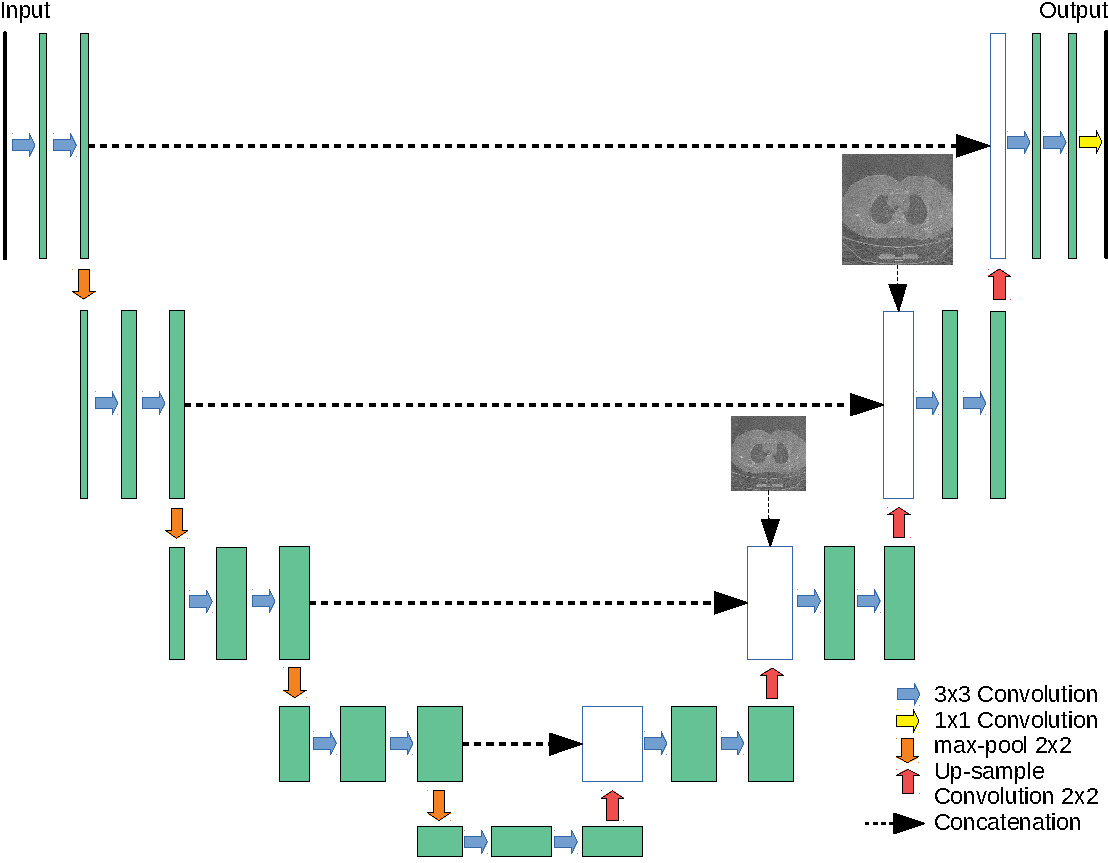
\includegraphics[width=0.8\linewidth]{./Figures/u_net-crop.pdf}
	\caption{\ac{LRRCED}(U): U-Net with $\boldx_1$ at $128\times128$ and $\boldx_2$ at $256\times256$.}
	\label{fig:un}
\end{figure}

\subsubsection{Loss Function}
The aim of a supervised data-driven image reconstruction task is to predict an image that is as close as possible to the \ac{GT} image. The appropriate loss function to achieve this is the \ac{MAE} which is defined as follows:
\begin{equation}
\mathrm{MAE}(\boldx^\star, \boldxhat) = \frac{1}{m}   \sum_{j=1}^m |x^\star_j - \hat{x}_j|
\end{equation}
where $\boldx^\star =  [x_1^\star, \dots , x_m^\star]^\top \in \mathbb{R}^m$ and $\boldxhat= [\hat{x}_1, \dots , \hat{x}_m]^\top \in \mathbb{R}^m$ are respectively the true image and predicted image.

In order to improve the resolution of reconstructed images, many deep learning approaches have used the perceptual loss as proposed by \cite{johnson2016perceptual}. This loss uses a pre-trained neural network to extract features from the predicted image and the \ac{GT}. It can be defined as follows:

\begin{equation}
P_k(\boldx^\star,\boldxhat) =  |[\mathrm{VGG16}]_k(\boldx^\star) - [\mathrm{VGG16}]_k( \boldxhat)|, \quad k =1,\dots,5 \,  
\end{equation}
where $[\mathrm{VGG16}]_k(\boldx^\star)$ and $[\mathrm{VGG16}]_k( \boldxhat)$ are the features extracted from block $k$ of the $\mathrm{VGG16}$ neural network \cite{simonyan2014very} with respectively the \ac{GT} and the predicted image as inputs. The features extracted from higher layers of the neural network contain generic information (edges, contrast, etc.) while the deeper layers have finer task-specific details. The VGG16 network was pre-trained on Image-Net data \cite{deng2009imagenet} which is far from a medical context. Hence, the higher-level generic features were found to be more relevant for the task of medical image reconstruction. We observed that using extracted features from two different levels, namely Block 1 and Block 3, of the VGG16 network proved to be most effective. 

The final loss function that was used for training both the aforementioned networks is defined as follows: 
\begin{equation}\label{eq:loss}
\mathcal{L}(\boldx^\star,\boldxhat) = \alpha\mathrm{MAE}(\boldx^\star, \boldxhat)+\beta(P_{1}(\boldx^\star,\boldxhat)+P_{3}(\boldx^\star,\boldxhat))
\end{equation}
where $P_{1}$ and $P_{3}$ are perceptual loss from the extracted features of the two different blocks above-mentioned, $\alpha$ and $\beta$ are weights which were set to $0.5$ and $10$ during the training phase.  


\section{Dataset}
The data used in this work is from the \ac{Lung} \cite{Lung20,clark2013cancer}. Details of the dataset are given in Table~\ref{table:2a}. The images in this dataset were reconstructed using \ac{FBP} on full-angular coverage measurement data. We used the ASTRA toolbox \cite{van2016fast}, for data processing to create the projection-image pairs.  A fan-beam geometry with a source to detector distance at $1500$ mm and source to the center of the rotation at $1000$ mm were considered. The number of detectors was set to $700$ and the number of angles was varied to generate different levels of sparsity ($N_\mathrm{a}=60,90$ and $120$). The noise-free projection data were obtained using the Beer-Lambert law \eqref{eq:CT} with an input emission intensity of $10^5$. The final projection data were obtained by adding Poisson noise (i.e., \eqref{eq:poisson}) to the noise-free projection data. We finally generated the \ac{FBP} estimates from the noise-added sparse-projections which were used in training the networks as explained previously. Sample images from the dataset are shown in Figure~\ref{fig:data}. 



\begin{table}[ht!]
	\caption{Dataset Description}
	\label{table:2a}
	\centering
	\begin{tabular}{||c|c||} 
		\hline
		Dataset Statistics &  \\ [0.5ex] 
		\hline
		Modalities & CT, PET   \\ 
		\hline
		Number of Participants  & 355  \\
		\hline
		Number of Studies  & 436  \\
		\hline
		Number of Series & 1295 \\ 
		\hline
		Number of 2-D Image slices & 251,135 \\ 
		\hline
		PET Matrix size & 200 \\ 
		\hline
		CT Matrix size & 512 \\ 
		\hline
		
	\end{tabular}
	
\end{table}

\begin{figure}[!htbp]
	\centering
	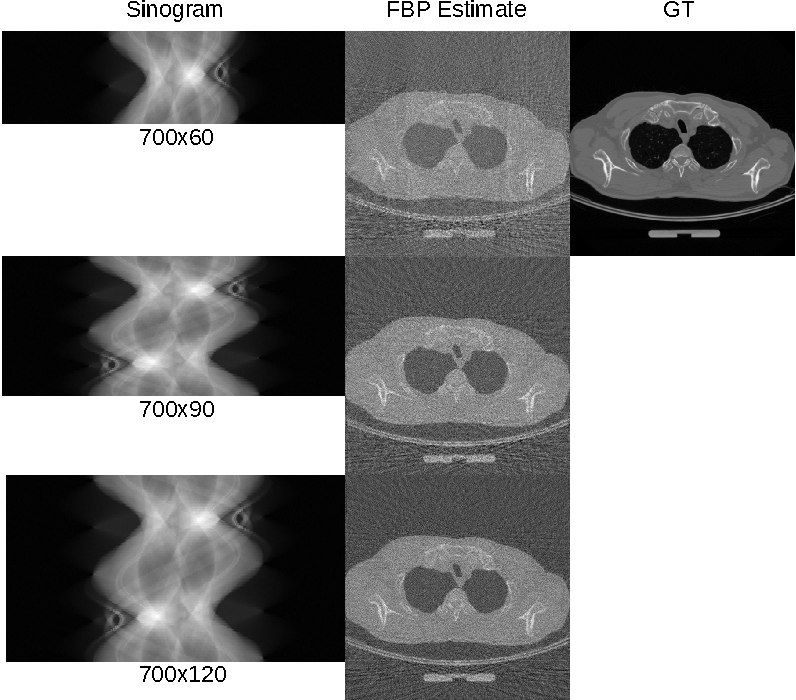
\includegraphics[width=0.8\linewidth]{./Figures/data-crop.pdf}
	\caption{Samples from the dataset: Sinograms with different sparse-view configurations along with their corresponding \ac{FBP} estimate.}
	\label{fig:data}
\end{figure}


\section{Training}

We implemented the architectures described in the previous section using TensorFlow \cite{abadi2016tensorflow} and Keras \cite{chollet2015keras}. A subset of the dataset consisting of 22,000 \ac{2D} \ac{CT} images was used in this study. We then split the data into 20,000 images for training and 2,000 images for testing. The sinograms and \ac{FBP} estimates were generated using the ASTRA toolbox as described above. The sinograms were resized to $512 \times 512$ to ensure symmetry with the images for easier training of the network. The \ac{FBP} estimates $\boldxhat_1$ and $\boldxhat_2$ were resized to the resolutions required for concatenation to the proposed networks. The neural networks were independently trained for each of the sparse-view settings with $N_\mathrm{a}=60,90$ and $120$. The choice of $\boldx_1$ and $\boldx_2$ were at $64\times64$ and $128\times128$ resolutions for \ac{LRRCED}(D) and $128\times128$ and $256\times256$ resolutions for \ac{LRRCED}(U). The networks were trained for 25 epochs with Adam optimizer with a decay of $10^{-4}$.


\section{Quantitative Analysis:}

The metrics used for evaluating the reconstructed images were \ac{SSIM} and \ac{PSNR}. They are defined as follows:
\begin{equation}
\mathrm{SSIM}(\boldx^\star,\boldx) = \frac{(2\mu_{\boldx^\star}\mu_{\boldx}+c_{1})(2\sigma_{\boldx^\star\boldx}+c_{2})}{(\mu_{\boldx^\star}^2+\mu_{\boldx}^2+c_{1})(\sigma_{\boldx^\star}^2+\sigma_{\boldx}^2+c_{2})}   
\end{equation}
where $\mu_{\boldx^\star}$ and $\mu_{\boldx}$ are the mean of $\boldx^\star$ and $\boldx$ respectively, $\sigma_{\boldx^\star}^2$ and $\sigma_{\boldx}^2$ are the variance of $\boldx^\star$ and $\boldx$, $\sigma_{\boldx^\star\boldx}$ is the covariance between $\boldx^\star$ and $\boldx$ , $c_{1}=(k_{1}L)^2$ and $c_{2}=(k_{2}L)^2$ where $k_{1}=0.01$ and $k_{2}=0.03$ by default,
\begin{equation}
\mathrm{PSNR} = 20\log_{10}\left(\frac{L-1}{\mathrm{RMSE}}\right)
\end{equation}
where $L$ is the maximum intensity in the image and \ac{RMSE} is given by
\begin{equation}
%    \mathrm{RMSE}(Y_\mathrm{true},Y_\mathrm{predicted}) = \sqrt{\frac{1}{n}   \sum_{i=1}^{n} (Y_\mathrm{true}^i-Y_\mathrm{predicted}^i)^2} 
\mathrm{RMSE}(\boldx^\star,\boldxhat) = \sqrt{\frac{1}{m}   \sum_{j=1}^{m} (x^\star_j-\xhat_j )^2} \, .
\end{equation}



\section{Comparative Analysis}

The  \ac{LRRCED} method was compared with a post-processing deep learning-based approach, namely FBP-ConvNet \cite{jin2017deep}, and a \ac{PWLS}-\ac{TV} solver for the model-based iterative \ac{CT} reconstruction \cite{tang2009performance}. We trained FBP-ConvNet on a set of 20,000 noisy, artifact-ridden \ac{FBP} image and \ac{GT} pairs. This network was trained for 25 epochs. 

\section{Results} \label{sec:results}

\subsection{Experimental Results}

Figure~\ref{fig:d_ang} shows the images reconstructed with \ac{LRRCED}(D) for various degrees of sparsity in the projections. Also given below each image is the \ac{SSIM} and \ac{PSNR} w.r.t. \ac{GT}. The region enclosed in the yellow box is further zoomed in for clearer inspection. As the sparsity in the views reduces, the \ac{SSIM} and \ac{PSNR} also improve. Similarly in Figure~\ref{fig:u_ang}, we show the images reconstructed with \ac{LRRCED}(U). Similar to the previous case, we observe improvements in the metrics as the sparsity decreases. 

In Figure~\ref{fig:res_60} and Figure~\ref{fig:res_90} we present a comparison of reconstructed images with different algorithms with 60 views and 90 views respectively. The top row consists of the \ac{GT} and the proposed \ac{LRRCED}(D) and \ac{LRRCED}(U) approaches. The second row consists of FBP-ConvNet, \ac{PWLS}-\ac{TV} iterative method and \ac{FBP}. The region highlighted in yellow is zoomed and corresponding images are displayed in the third and fourth rows. These methods are quantitatively compared in Table~\ref{table:3} and Table~\ref{table:4}. We observe that the deep learning methods perform better than the iterative and analytical methods. The proposed approach has the best metrics for projections with 90 views. The deep learning-based methods have similar metrics in the 60-view scenario. The intensity line profiles of the regions marked in red in Figure~\ref{fig:res_60} and Figure~\ref{fig:res_90} are plotted in Figure~\ref{fig:ip_60} and Figure~\ref{fig:ip_90} respectively. In accordance with the metrics tabulated in Table~\ref{table:3} and Table~\ref{table:4}, we find that the plots of deep learning-based methods are very close to that of the \ac{GT}. Even though the proposed approach with typical \acp{CED} performs a task which is more complex than denoising, the metrics indicate that the quality has not deteriorated compared to a standard post-processing approach. The inclusion of perceptual loss in \ref{eq:loss} was to improve the sharpness of the reconstructed images. This is indeed reflected in the images predicted by the proposed approach but we also observe some artifacts (regularly spaced white dots) in the images (especially for 60 views).

\begin{figure}[!htbp]
	\centering
	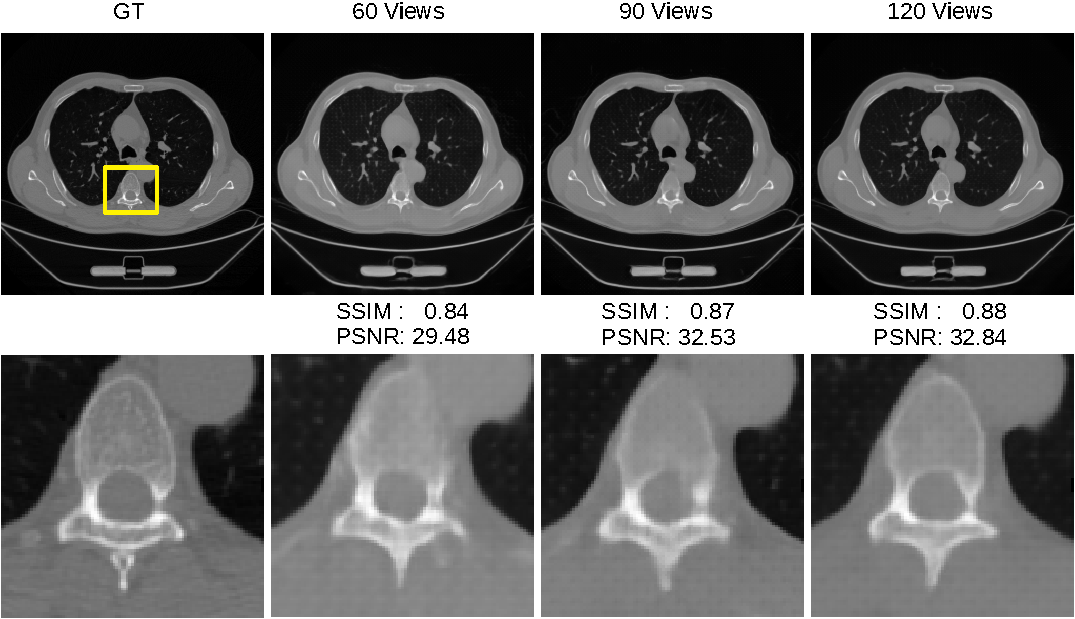
\includegraphics[width=0.8\linewidth]{./Figures/views_dense-crop.pdf}
	\caption{Images reconstructed with LRR-CED(D) approach with different sparse-view configurations, i.e., projections with $N_\mathrm{a}=60,90$ and $120$.}
	\label{fig:d_ang}
\end{figure}


\begin{figure}[!htbp]
	\centering
	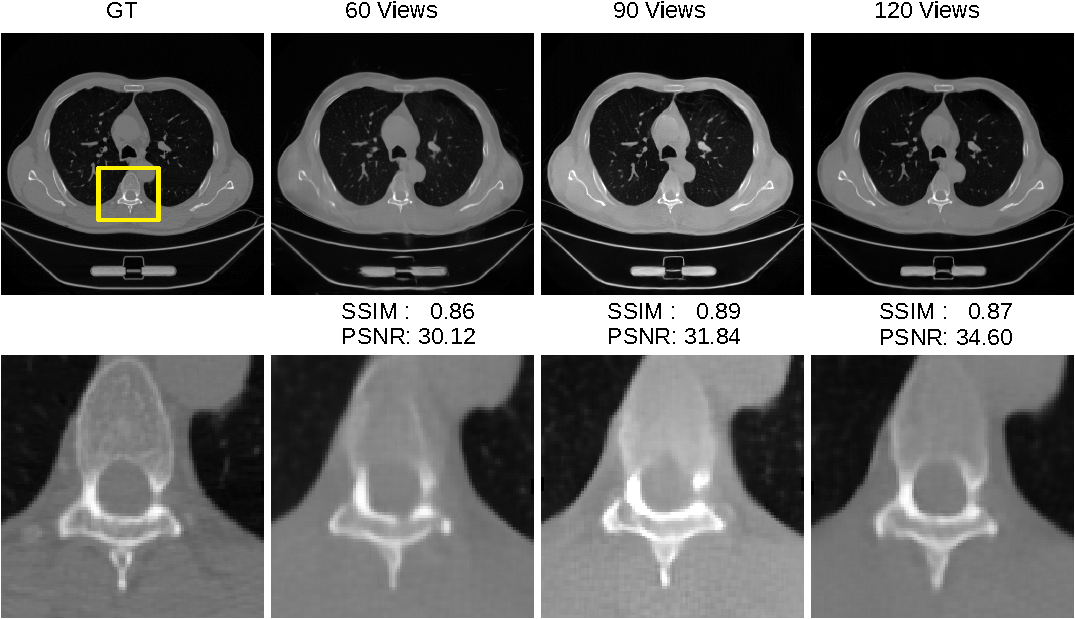
\includegraphics[width=0.8\linewidth]{./Figures/views_unet-crop.pdf}
	\caption{Images reconstructed with LRR-CED(U) approach with different Sparse-View configurations, i.e., projections with $N_\mathrm{a}=60,90$ and $120$.}
	\label{fig:u_ang}
\end{figure}


\begin{table}[ht!]
	\centering
	\caption{Quantitative comparison of various reconstruction algorithms with \ac{SSIM} and \ac{PSNR} for projections with 60 views}
	\label{table:3a}
	\begin{tabular}{||c|c|c|c|c|c||} 
		\hline
		Metric & FBP & PWLS-TV & FBP & \ac{LRRCED} & \ac{LRRCED}  \\ %[0.5ex] 
		&     &         & ConvNet & (D) & (U) \\
		\hline\hline
		SSIM & $0.16$ & $0.66$ & $0.85$ & $0.84$ & $0.87$ \\ 
		PSNR & $11.57$ & $28.23$ & $31.52$ & $29.48$ & $30.12$ \\   
		\hline  
		
		\hline  
	\end{tabular}
	
\end{table}

\begin{table}[ht!]
	\centering
	\caption{Quantitative comparison of various reconstruction algorithms with \ac{SSIM} and \ac{PSNR} for projections with 90 views}
	\label{table:4a}
	\begin{tabular}{||c|c|c|c|c|c||} 
		\hline
		Metric & FBP & PWLS-TV & FBP & \ac{LRRCED} & \ac{LRRCED}  \\ %[0.5ex] 
		&     &         & ConvNet & (D) & (U) \\
		\hline\hline
		SSIM & $0.19$ & $0.72$ & $0.81$ & $0.88$ & $0.89$ \\ 
		PSNR & $13.57$ & $30.21$ & $31.45$ & $32.53$ & $31.84$ \\   
		\hline  
		
		\hline  
	\end{tabular}
	
\end{table}



\begin{figure}[!t]
	\centering
	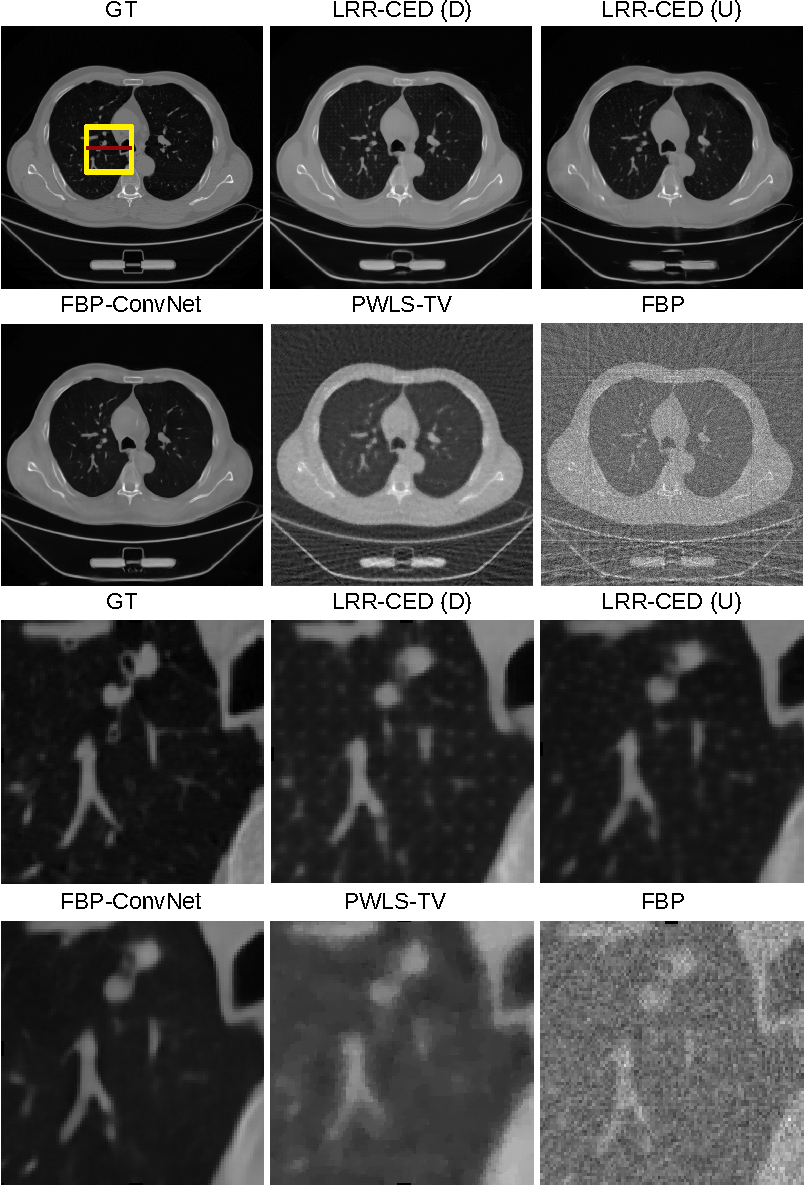
\includegraphics[width=1.0\linewidth]{./Figures/results1-crop.pdf}
	\caption{Comparative analysis for 60 views: From the top left, we have \ac{GT} image, reconstructions with \ac{LRRCED}(D) and \ac{LRRCED}(U). In the second row reconstructed images with FBP-ConvNet, PWLS-TV and \ac{FBP}. }
	\label{fig:res_60}
\end{figure}

\begin{figure}[!t]
	\centering
	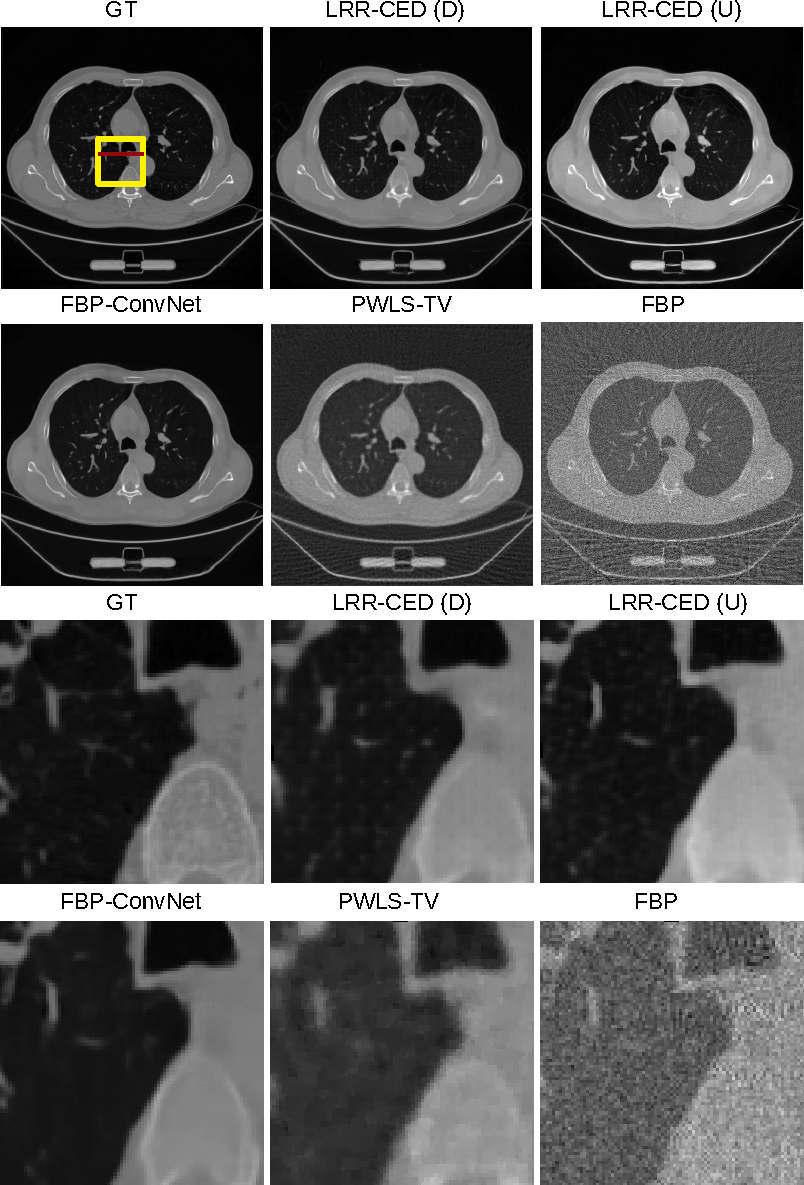
\includegraphics[width=1.0\linewidth]{./Figures/result2-crop.pdf}
	\caption{Comparative analysis for 90 views: From the top we have \ac{GT} image, reconstructions with \ac{LRRCED}(D) and \ac{LRRCED}(U). In the second row reconstructed images with FBP-ConvNet, PWLS-TV and \ac{FBP}.}
	\label{fig:res_90}
\end{figure}

\begin{figure}[!h]
	\centering
	\begin{tikzpicture}[scale=1] 
	\begin{axis}[
	% title=X-ray source Energy: $140$ keV,
	mark options={mark size = 3pt},
	xlabel={Distance (in pixels)},
	ylabel={Normalized Attenuation (mm$^{-1}$)},
	xmin = 200,
	xmax = 300,
	grid = major,
	legend columns=2,
	legend cell align=left,
	legend entries={PWLS-TV,\ac{GT},\ac{LRRCED}(D),\ac{LRRCED}(U),FBP-ConvNet},
	% legend entries={MCAOL,CAOL, Huber, TV, },
	legend style={at={(0.5,1.2)},anchor=north}
	]
	
	\addplot[color=blue, style={thick}] table[x=Distance, y=PWLS-TV] {./Plots/Fig11.txt};
	\addplot[color=green, style={thick}] table[x=Distance, y=GT] {./Plots/Fig11.txt};
	\addplot[color=red, style={thick}] table[x=Distance, y=LRR-CED(D)] {./Plots/Fig11.txt};
	\addplot[color=magenta, style={thick}] table[x=Distance, y=LRR-CED(U)] {./Plots/Fig11.txt};
	\addplot[color=black, style={thick}] table[x=Distance, y=FBP-ConvNet] {./Plots/Fig11.txt};
	\end{axis}
	\end{tikzpicture}
	
	\caption{Intensity plot profile for the region marked in red from Figure~\ref{fig:res_60} for PWLS-TV, \ac{GT}, \ac{LRRCED}(D), \ac{LRRCED}(U) and FBP-ConvNet.}\label{fig:ip_60}
\end{figure}

\begin{figure}[!h]
	\centering
	\begin{tikzpicture}[scale=1] 
	\begin{axis}[
	% title=X-ray source Energy: $140$ keV,
	mark options={mark size = 3pt},
	xlabel={Distance (in pixels)},
	ylabel={Normalized Attenuation (mm$^{-1}$)},
	xmin = 200,
	xmax = 300,
	grid = major,
	legend columns=2,
	legend cell align=left,
	legend entries={PWLS-TV,\ac{GT},\ac{LRRCED}(D),\ac{LRRCED}(U),FBP-ConvNet},
	% legend entries={MCAOL,CAOL, Huber, TV, },
	legend style={at={(0.5,1.2)},anchor=north}
	]
	
	\addplot[color=blue, style={thick}] table[x=Distance, y=PWLS-TV] {./Plots/Fig10.txt};
	\addplot[color=green, style={thick}] table[x=Distance, y=GT] {./Plots/Fig10.txt};
	\addplot[color=red, style={thick}] table[x=Distance, y=LRR-CED(D)] {./Plots/Fig10.txt};
	\addplot[color=magenta, style={thick}] table[x=Distance, y=LRR-CED(U)] {./Plots/Fig10.txt};
	\addplot[color=black, style={thick}] table[x=Distance, y=FBP-ConvNet] {./Plots/Fig10.txt};
	\end{axis}
	\end{tikzpicture}
	
	\caption{Intensity plot profile for the region marked in red from Figure~\ref{fig:res_90} for PWLS-TV, \ac{GT}, \ac{LRRCED}(D), \ac{LRRCED}(U) and FBP-ConvNet.}\label{fig:ip_90}
\end{figure}


\subsection{Hyperparameter optimization}

Finding the optimal hyperparameters is an important aspect of training neural networks. The common hyperparameters in a typical \ac{CNN} are number of filters, number of layers, etc. These interdependent hyperparameters  determine the rate of convergence and require task-specific experimentation to arrive at the best possible configuration. The unique hyperparameters in our proposed approach are the resolutions of concatenated \ac{FBP} estimates. The number of training examples is another important component that varies depending on the task and the trainable parameters of the neural network selected for the task. In this section we discuss our experiments that determined the selection of these two important hyperparameters. 

\subsubsection{Concatenation Resolution Selection} \label{sec:concat}

To select the best possible configuration for concatenation in the proposed approach, we trained the networks with a fixed set of hyper-parameters and different combinations of concatenations. We discuss the results with \ac{LRRCED}(D) in this regard. The number of training samples were set to 10,000 for all the experiments. The training data were projections with 90 views, corresponding \ac{FBP} reconstructed images and the \ac{GT}. The training was done for 25 epochs. Each of the concatenation setting was evaluated on 5 test patients. The average \ac{SSIM} for each patient was plotted for each of the experiment setting. In Fig~\ref{fig:c1} we have the average \ac{SSIM} vs Patient plot for single concatenation at a specific resolution. Similarly Figure~\ref{fig:c2} consists of plots for double concatenation at two different resolutions. The double concatenation at $64\times64, 128\times128$ overall leads to the best metrics, thus becoming our choice for the experiments in this work. These results are tabulated in Table~\ref{table:5}.



\subsubsection{Training Examples Analysis}

One of the biggest challenges in any data driven algorithm is the selection of training examples required for the experiments. It is important to analyze this hyper-parameter as it serves as an important factor for the network to be reproducible and scalable. We varied the number of training examples for the best concatenation setting from the previous section and the 90-view scenario. The evaluation was similar to the previous experiment with the average \ac{SSIM} for 5 patients. The results from these experiments are tabulated in Table~\ref{table:6}. As seen in Figure~\ref{fig:tr}, the performance of the network improves along with the increase in the number of training examples. There is however a marginal difference in the performance of the network when trained with 20,000 or 30,000 training examples, hence making us choose 20,000 training examples as the optimum number for this hyper-parameter. The average \ac{SSIM} values across the test patients tend to get similar as the number of training examples increases.




\begin{table}[ht!]
	\centering
	\caption{Average \ac{SSIM} for different configurations of concatenations}
	\label{table:5}
	\begin{tabular}{||c|c|c|c|c|c||} 
		\hline
		Concatenated & \multicolumn{5}{c||}{Average \ac{SSIM}}  \\ \cline{2-6}%[0.5ex] 
		\ac{FBP} Resolution &   P1  &  P2     & P3 & P4 & P5 \\
		\hline\hline
		$(32\times32)$ & $0.82$ & $0.86$ & $0.88$ & $0.86$ & $0.80$ \\ 
		$(64\times64)$ & $0.85$ & $0.88$ & $0.90$ & $0.88$ & $0.82$ \\   
		$(128\times128)$ & $0.85$ & $0.87$ & $0.90$ & $0.89$ & $0.81$ \\   
		$(256\times256)$ & $0.58$ & $0.88$ & $0.85$ & $0.88$ & $0.79$ \\   
		$(512\times512)$ & $0.66$ & $0.78$ & $0.82$ & $0.75$ & $0.73$ \\   
		\hline
		$(32\times32,64\times64)$ & $0.83$ & $0.77$ & $0.80$ & $0.80$ & $0.68$ \\   
		$\mathbf{(64\times64,128\times128)}$ & $\mathbf{0.85}$ & $\mathbf{0.88}$ & $\mathbf{0.91}$ & $\mathbf{0.89}$ & $\mathbf{0.83}$ \\   
		$(128\times128,256\times256)$ & $0.67$ & $0.78$ & $0.83$ & $0.84$ & $0.70$ \\   
		\hline  
		
		\hline  
	\end{tabular}
	
\end{table}

\begin{table}[ht!]
	\centering
	\caption{Average \ac{SSIM} for different number of training examples}
	\label{table:6}
	\begin{tabular}{||c|c|c|c|c|c||} 
		\hline
		Number of Training  & \multicolumn{5}{c||}{Average \ac{SSIM}}  \\ \cline{2-6}%[0.5ex] 
		examples &   P1  &  P2     & P3 & P4 & P5 \\
		\hline\hline
		$1,000$ & $0.82$ & $0.79$ & $0.86$ & $0.85$ & $0.72$ \\ 
		$5,000$ & $0.84$ & $0.77$ & $0.86$ & $0.84$ & $0.69$ \\   
		$10,000$ & $0.85$ & $0.88$ & $0.91$ & $0.89$ & $0.83$ \\   
		$\mathbf{20,000}$ & $\mathbf{0.89}$ & $\mathbf{0.90}$ & $\mathbf{0.91}$ & $\mathbf{0.90}$ & $\mathbf{0.82}$ \\   
		$30,000$ & $0.89$ & $0.89$ & $0.90$ & $0.90$ & $0.82$ \\   
		\hline  
		
		\hline  
	\end{tabular}
	\vspace{.5cm}
\end{table}



\begin{figure}[!h]
	\centering
	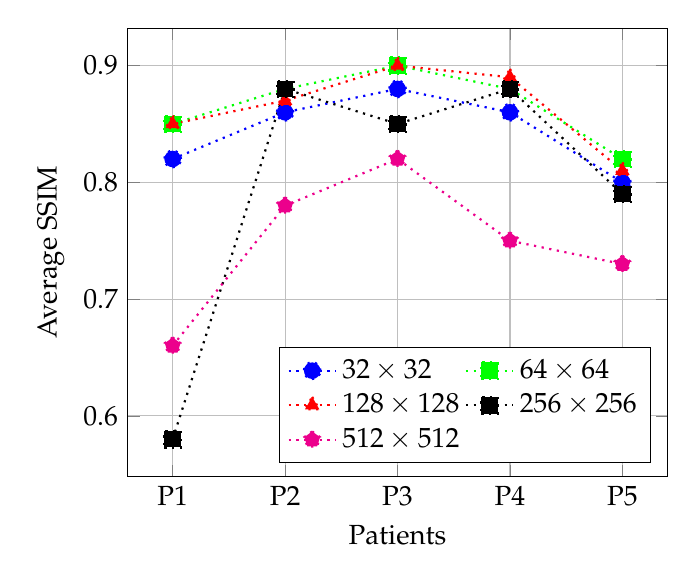
\begin{tikzpicture}[scale=1] 
	\begin{axis}[
	% title=X-ray source Energy: $140$ keV,
	mark options={mark size = 3pt},
	xlabel={Patients},
	ylabel={Average SSIM},
	xticklabels={,P1,P2,P3,P4,P5},
	grid = major,
	legend columns=2,
	legend cell align=left,
	legend entries={$32\times 32$,$64\times 64$,$128\times 128$,$256\times 256$,$512\times 512$},
	% legend entries={MCAOL,CAOL, Huber, TV, },
	legend style={legend pos=south east}
	]
	
	\addplot[color=blue, mark=*, style={thick,dotted}] coordinates   {(0,0.82)(10,0.86)(20,0.88)(30,0.86)(40,0.8)};
	\addplot[color=green, mark=square*, style={thick,dotted}] coordinates  {(0,0.85)(10,0.88)(20,0.9)(30,0.88)(40,0.82)};
	\addplot[color=red, mark=triangle*, style={thick,dotted}] coordinates  {(0,0.85)(10,0.87)(20,0.9)(30,0.89)(40,0.81)};
	\addplot[color=black, mark=square*, style={thick,dotted}] coordinates    {(0,0.58)(10,0.88)(20,0.85)(30,0.88)(40,0.79)};
	\addplot[color=magenta, mark=pentagon*, style={thick,dotted}] coordinates {(0,0.66)(10,0.78)(20,0.82)(30,0.75)(40,0.73)};
	
	\end{axis}
	\end{tikzpicture}
	
	\caption{Comparison of single concatenations for the particular case of 90 views evaluated with \ac{SSIM} on 5 different patients from the dataset. The best metrics are found with concatenation at $128\times 128$.}\label{fig:c1}
\end{figure}



\begin{figure}[!htbp]
	\centering
	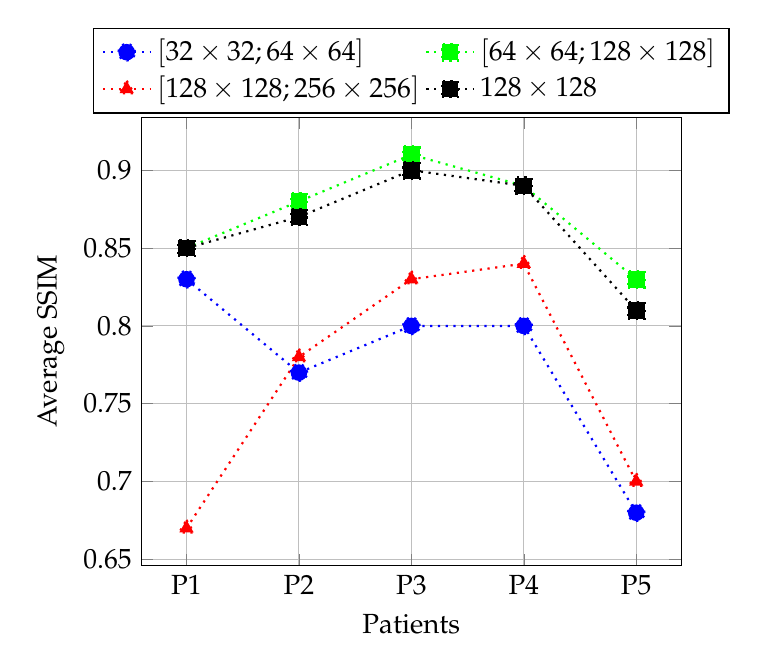
\begin{tikzpicture}[scale=1] 
	\begin{axis}[
	% title=X-ray source Energy: $140$ keV,
	mark options={mark size = 3pt},
	xlabel={Patients},
	ylabel={Average SSIM},
	xticklabels={,P1,P2,P3,P4,P5},
	grid = major,
	legend columns=2,
	legend cell align=left,
	legend entries={$[32\times 32 ; 64\times 64]$,$[64\times 64 ; 128\times 128]$,$[128\times 128 ; 256\times 256]$,$128\times 128$},
	% legend entries={MCAOL,CAOL, Huber, TV, },
	legend style={at={(0.5,1.2)},anchor=north}
	]
	
	\addplot[color=blue, mark=*, style={thick,dotted}] coordinates   {(0,0.83)(10,0.77)(20,0.8)(30,0.8)(40,0.68)};
	\addplot[color=green, mark=square*, style={thick,dotted}] coordinates  {(0,0.85)(10,0.88)(20,0.91)(30,0.89)(40,0.83)};
	\addplot[color=red, mark=triangle*, style={thick,dotted}] coordinates  {(0,0.67)(10,0.78)(20,0.83)(30,0.84)(40,0.7)};
	\addplot[color=black, mark=square*, style={thick,dotted}] coordinates    {(0,0.85)(10,0.87)(20,0.9)(30,0.89)(40,0.81)};
	
	\end{axis}
	\end{tikzpicture}
	
	\caption{Comparison of double concatenations for the particular case of 90 views evaluated with \ac{SSIM} on 5 different patients from the dataset. The best metrics are found with concatenations at $64\times 64$ and $128\times 128$ resolutions.}\label{fig:c2}
\end{figure}


\begin{figure}[!h]
	\centering
	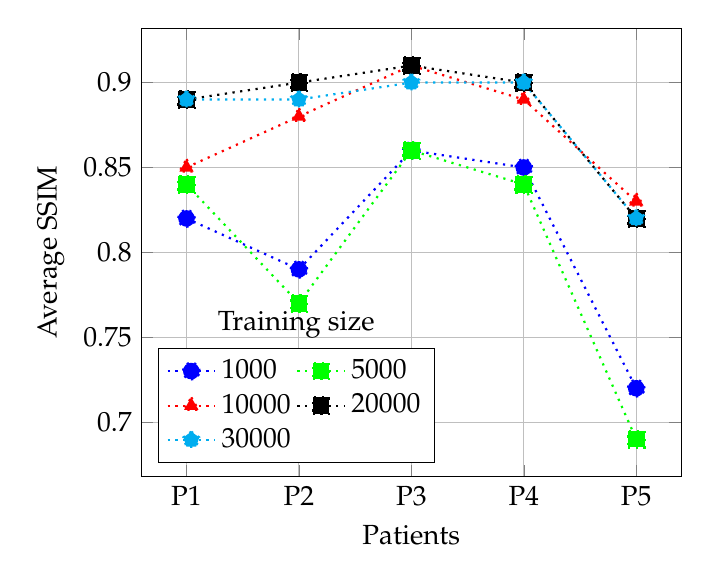
\begin{tikzpicture}[scale=1] 
	\begin{axis}[
	% title=X-ray source Energy: $140$ keV,
	mark options={mark size = 3pt},
	xlabel={Patients},
	ylabel={Average SSIM},
	xticklabels={,P1,P2,P3,P4,P5},
	grid = major,
	legend columns=2,
	legend cell align=left,
	legend entries={$1000$,$5000$,$10000$,$20000$,$30000$},
	% legend entries={MCAOL,CAOL, Huber, TV, },
	legend style={legend pos=south west,label=above:Training size}
	]
	
	\addplot[color=blue, mark=*, style={thick,dotted}] coordinates   {(0,0.82)(10,0.79)(20,0.86)(30,0.85)(40,0.72)};
	\addplot[color=green, mark=square*, style={thick,dotted}] coordinates  {(0,0.84)(10,0.77)(20,0.86)(30,0.84)(40,0.69)};
	\addplot[color=red, mark=triangle*, style={thick,dotted}] coordinates  {(0,0.85)(10,0.88)(20,0.91)(30,0.89)(40,0.83)};
	\addplot[color=black, mark=square*, style={thick,dotted}] coordinates    {(0,0.89)(10,0.9)(20,0.91)(30,0.9)(40,0.82)};
	\addplot[color=cyan, mark=pentagon*, style={thick,dotted}] coordinates {(0,0.89)(10,0.89)(20,0.9)(30,0.9)(40,0.82)};
	
	\end{axis}
	\end{tikzpicture}
	
	\caption{Comparison of Average \ac{SSIM} for 5 different Patient data for 90 views with varying number of training samples. The configuration of the network is the one with best performance from the analysis in Figure~\ref{fig:c1}. (concatenations at $64\times 64$ and $128\times 128$). }\label{fig:tr}
\end{figure}



\section{Discussion} \label{sec:discussion}

The use of deep learning architectures in the framework of medical image reconstruction is propelled by potentially faster reconstruction without compromising on the quality of the images. To this end, hybrid image reconstruction involving unrolled iterative algorithms with embedded deep learning architectures do not significantly reduce the reconstruction time. Hence, the use of deep learning architectures for either improving images from a fast analytic algorithm or direct reconstruction becomes more relevant for their incorporation into the image reconstruction pipeline. One significant problem for direct image reconstruction is the requirement of large and complex networks to learn the mapping from sinograms to images without the help of any reconstruction estimate. The networks used for post-processing on the other hand are simpler and relatively easy to train. In this work we attempted to use these post-processing networks for the direct image reconstruction task. We show that concatenating \ac{FBP} estimates at lower resolutions is sufficient to allow the network to learn the mapping from sinogram to image space. Through the use of two different networks with the concatenation approach we demonstrate that this idea can be applied to \acp{CED} in general.   

In the sparse-view \ac{CT} scenario artifact removal along with denoising increases the challenges of getting a clean well-resolved image. We observed that the use of traditional loss functions (L1 or L2) resulted in blurry images. To tackle this and to improve the sharpness of the images we used perceptual loss along with the standard L1 loss. The reconstructed images with our proposed \ac{LRRCED}(D) and \ac{LRRCED}(U) have higher \ac{SSIM} and \ac{PSNR} than images reconstructed with a traditional iterative algorithm. The evaluation metrics were very close to a standard post-processing deep learning method FBP-ConvNet. This similarity stems from the fact that the choice of networks used in our proposed work was inspired from post-processing \acp{CED}. The contribution in this work is the use of these networks to learn the mapping from sparse sinograms to images with the same amount of training examples, which is possible only with the proposed addition of the concatenations.  

We are currently exploring the possibility of using image estimates from earlier iterations of standard iterative algorithms while ensuring that the trade-off between time and image quality is not compromised. The use of other alternative architectures is also being explored to arrive at reconstructed images which perform significantly better than existing post-processing approaches. Finally, we are working on experiments with low-dose \ac{CT} and other tomographic reconstruction modalities to establish the adaptability of the proposed approach.  

\section{Conclusion} \label{sec:conclusion}

In this work we studied the use of fully convolutional encoder-decoder networks in direct sparse-\ac{CT} image reconstruction. We introduced a new approach that uses lower dimension \ac{FBP} estimates as concatenations to help the network learn the mapping from sinogram to image space. In the context of image reconstruction, we inject the information from the inverse of a \ac{CT} physical system (\ac{FBP} estimate) as a feature map in the decoder. We presented two variations of the proposed approach namely \ac{LRRCED}(D) using fully convolutional dense networks and \ac{LRRCED}(U) using U-Net. The proposed neural networks reconstruct images that are either better or are on par with traditional reconstruction algorithms and post-processing deep learning based approach (FBP-ConvNet). A single pass of a sparse sinogram through the network results in reconstructed images without the artifacts and noise which are severely present in the concatenated \ac{FBP} estimates. Finally, this idea of using task specific concatenations that enable one to have control over what the network learns, can be extended to various other problems in medical imaging. 


 
% Chapter 4

\chapter{LRR-CED: Low-Resolution Reconstruction aware Convolutional Encoder-Decoder Network  for Direct Sparse-View CT Image Reconstruction} % Main chapter title
\chaptermark{LRRCED}
\label{Chapter4} % For referencing the chapter elsewhere, use \ref{Chapter1} 

Sparse-view \ac{CT} reconstruction has been at the forefront of research in medical imaging. Reducing the total X-ray radiation dose to the patient while preserving the reconstruction accuracy is a big challenge. The sparse-view approach is based on reducing the number of rotation angles, which leads to poor quality reconstructed images as it introduces several artifacts. These artifacts are more clearly visible in traditional reconstruction methods like the \ac{FBP} algorithm. Over the years, several model-based iterative and more recently deep learning-based methods have been proposed to improve sparse-view \ac{CT} reconstruction. Many deep learning-based methods improve \ac{FBP}-reconstructed images as a post-processing step. In this work, we propose a direct deep learning-based reconstruction that exploits the information from low-dimensional \ac{FBP} estimates, to learn the  projection-to-image mapping. This is done by concatenating the \ac{FBP} estimate at multiple resolutions in the decoder part of a \ac{CED}. This approach is investigated on two different networks, based on Dense Blocks and U-Net to show that a direct mapping can be learned from a sinogram to an image.  The results are compared to a post-processing deep learning method and an iterative method that uses a \ac{TV} regularization. 


\section{Main Contribution}

The main drawbacks of current deep learning-based direct image reconstruction algorithms are the tedious training process necessary to train large networks with large number of trainable parameters and the requirement of high memory in case of high-resolution \ac{CT} images. 
In this work we propose a new method for direct deep learning based sparse-view \ac{CT} image reconstruction with fully convolutional networks. We use two networks, namely Fully Convolutional Densenets \cite{jegou2017one} and U-Net \cite{ronneberger2015u}. An important characteristic of both these architectures \cite{jegou2017one,ronneberger2015u} is the presence of concatenation from the encoding layers to the decoding layers that ensures the usage of features from the input for the reconstruction. Specifically, for application in sparse-\ac{CT} image reconstruction, the network would have sparse-view sinograms as input and reconstructed images as output. The original application in the medical imaging field of both these architectures was in image segmentation, where the image-to-image mapping operates in the same image domain. Medical image reconstruction on the other hand involves mapping between two different domains (sinogram to image). In order to help the network to learn the mapping from sinogram to image, we propose the use of \ac{FBP} image estimates of the sparse sinograms and concatenate them with the feature maps of the decoder. 

% \AP{Here the motivation for this "intuition" should be stated maybe you can introduce some simple notation already here: Given that we only have access to sparse measurement data (sinogram $\boldy$), we can enforce that the inverse mapping $f$ at each layer/ sub-resolution of the network is consistent in the measurement domain. That is 	$\boldL f(\boldy) = \boldy$.  this can be achieved by using concatenating as feature maps a (fast) low-resolution FBP for each or a subset of levels of the network. While this leads to a massive reduction of the parameters (number of layers) required in the network, the network parameters has to be trained accordingly since the above mentioned constraint is not enough to learn the inverse mapping, as it cannot capture information about the image $\boldx$ outside the range of the physical under-determined operator $\boldL$ (Radon transform for CT). Do not put details of the implementation in the introduction rather put the general idea behind.}

Given that we only have access to sparse measurement data, taking the form of a sinogram $\boldy$, we can enforce that the inverse mapping $\boldf$ at each layer/sub-resolution of the network is consistent in the measurement domain. That is $\boldP \boldf(\boldy) = \boldy$. This can be achieved by concatenating, as feature maps, (fast) low-resolution \ac{FBP}-reconstructed images for each or a subset of the network levels. While this leads to a massive reduction of the parameters (fully convolutional layers instead of fully-connected) required in the network, the above-mentioned constraint is not enough to learn the inverse mapping as it cannot capture information about the image $\boldx$ outside the range of the physical under-determined operator $\boldP$ (Radon transform for CT). Hence, the network needs to be trained accordingly.

Once the network is trained, these custom concatenations enable architectures that were previously used for denoising/artifact removal to learn a mapping from sparse sinograms to full-resolution \ac{CT} images. One characteristic feature of reconstructions generated by deep learning-based methods is the blurriness of the outputs. To counteract this we used perceptual loss involving features extracted from two different levels of $\mathrm{VGG16}$ network (Block 1 and Block 3). Since the exclusive use of perceptual loss results in unrealistic artifacts we couple it with a $L_1$ loss. A general representation of the proposed approach is depicted in Figure~\ref{fig:ge}. It consists of a \ac{CED} network with two blocks in both the encoder and the decoder that takes in as input a reshaped sparse sinogram which has the same dimensions as the output image. A concatenation of two resolutions $h_1 \times w_1$ and $h_2 \times w_2$ is incorporated in the decoder. 

The main contributions of our work are summarized as follows:
\begin{itemize}
	\item A new approach for sparse-view \ac{CT} image reconstruction using fully-convolutional networks
	\item Use of lower resolution \ac{FBP} estimates which enable the networks that are predominantly used for denoising to learn the more complex mapping from sinogram to image domain. 
	\item Two neural networks are implemented to test this approach using different levels of sparsity in the sinograms. 
\end{itemize}

\begin{figure}[!htbp]
	\centering
	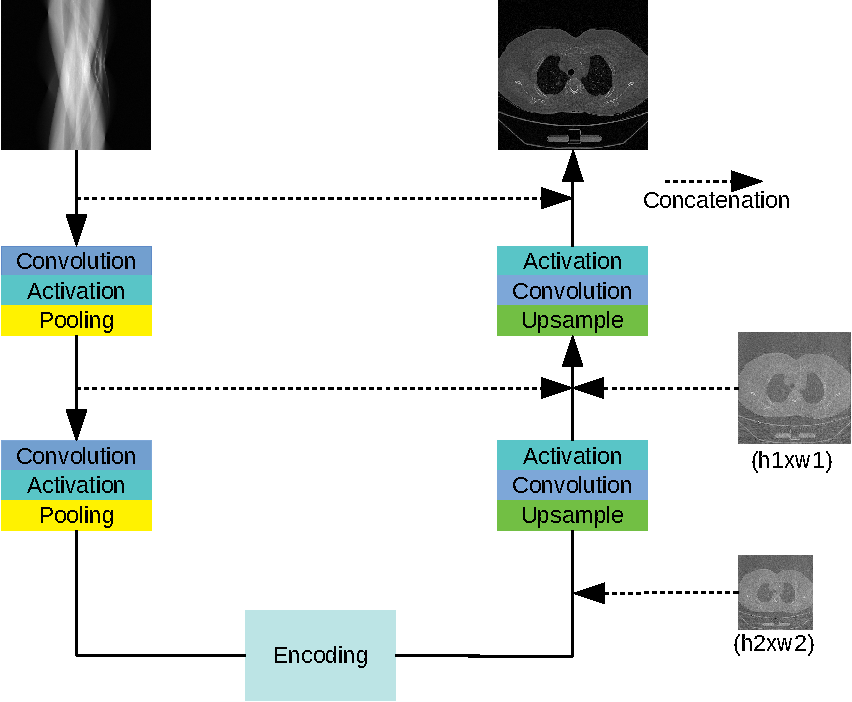
\includegraphics[width=0.7\linewidth]{general_enc-crop.pdf}
	\caption{General representation of an encoder-decoder architecture with fully convolutional layers and the proposed \ac{FBP} concatenations ($\boldx_1$ and $\boldx_2$) at two different resolutions $h_1 \times w_1$ and $h_2 \times w_2$}
	\label{fig:ge}
\end{figure}


\section{Methods}

\subsection{Proposed Low Resolution Reconstruction aware \ac{CED} Model}

Supervised deep learning-based methods learn the mapping between the measurement $\boldy$ and the corresponding reconstructed image $\boldx$. In the case of direct deep learning-based image reconstruction this mapping is typically learned via neural networks which can be represented as a function $\boldf_{\Theta}\colon \bbR^n \to \bbR^m$ with trainable parameters $\Theta$: 
\begin{equation}\label{eq:dl}
\boldxhat = \boldf_{\Theta}(\boldy) \, .
\end{equation}  
where, $\boldxhat$ is the predicted image. 

Most of the works in direct reconstruction for sparse-view \ac{CT} represent $\boldf$ with a neural network with fully-connected layers. These networks require huge memory and large datasets for training. As an alternative to this, we propose the use of fully convolutional encoder-decoder networks that have lesser trainable parameters and are faster to train. 
The main idea is to enforce data consistency by providing estimates at different resolutions $\boldxhat_r$, $r = 1, \ldots, R$:
\begin{equation}\label{eq:d}
\boldxhat = \boldf_{\Theta}(\boldy,   (\boldxhat_r)_{r=1}^R    ) 
\end{equation}  
where each $\boldxhat_r \in \bbR^{m_r}$, $m_r < m$, is an approximate solution of
\begin{equation}\label{eq:xr}
\boldy = \boldP \boldU_r \boldxhat_r
\end{equation} 
with $\boldU_r\in\bbR^{m\times m_r}$ being an upsampling operator.

In a typical \ac{CED}, the encoder learns the representation of the input domain and the decoder learns to map this representation to the corresponding image in the output domain. In the specific case of a \ac{CED} for medical image reconstruction, the encoder operates in the sinogram space and the decoder in the image space. Based on this hypothesis, we propose to concatenate the estimates at different levels of the decoder part of the network. The function of these concatenations is to help the network learn the structure of the image. The feature maps at different levels of the decoder have different resolutions. Hence, concatenating the estimate $\boldxhat_r$ at different levels requires the estimate to be of the appropriate resolution. The different convolutional layers in the decoder work towards arriving at a clear reconstructed image that is free of artifacts and noise. The estimate $\boldxhat_r$ is obtained with a sparse sinogram, hence it is artifact-ridden and noisy. Therefore, concatenating the estimate $\boldxhat_r$ at a level closer to the output resolution is counter productive as the network has lesser number of convolutional layers to correct the noise and artifacts. On the other hand the estimate at lower resolutions has lesser structural information compared to the estimates at higher resolution. The selection of $\boldxhat_r$ should ensure a balance between aiding the network to learn the structure of the image and enabling it to correct the artifacts and noise. 

Our method, namely \ac{LRRCED}, was implemented with $R=2$ and the image estimates $\boldxhat_r$ were obtained by \ac{FBP} at lower resolution. With the help of a series of experiments, we determined the best possible configuration for concatenating $\boldxhat_r$. In section Section~\ref{sec:concat}, we present quantitative evaluation of the effect of these concatenations on the reconstructed images. 

We investigate \ac{LRRCED} with two different variations for $\boldf$, \ac{LRRCED}(D) with Fully Convolutional DenseNets and \ac{LRRCED}(U) with U-Net, which are discussed in Section~\ref{sec:FCDN} and Section~\ref{sec:UNet}. 




\subsubsection{Fully Convolutional Dense Networks}\label{sec:FCDN}

A fully convolutional dense network was used as first variation of \ac{LRRCED}. Dense networks \cite{huang2017densely} are based on the hypothesis that connecting all the layers to each other in a feed forward fashion leads to higher accuracy and easier training of the network. A typical dense block of three layers is depicted in Figure~\ref{fig:db}. The extension of dense networks for image segmentation was proposed by \cite{jegou2017one}. The three  blocks involved in the construction of this network are \ac{DB} with $l$ number of layers, \ac{TU} and \ac{TD}. The combination of these three blocks helps in building an encoder-decoder structure suitable for tasks dealing with image-to-image domain transfer. Each layer consists of batch normalization, \ac{ReLU} activation and $3\times 3$ convolution. \ac{TD} includes: batch normalization, \ac{ReLU}, $1\times 1$ Convolution and $2\times 2$ max pooling. Finally, \ac{TU}  includes a $3\times 3$ transposed convolution with stride $2$. The important modification to the architecture blocks in our work is the removal of the dropout layers. The fully convolutional dense network with proposed concatenations is represented in Figure~\ref{fig:dn}. For the sake of representation we included only $5$ dense blocks in the figure. The complete architecture details are given in Table~\ref{table:1a}. 


\subsubsection{U-Net}\label{sec:UNet}

One of the most established architectures for image-to-image translation is U-Net \cite{ronneberger2015u}, which we used as second variation of \ac{LRRCED} (called from here on-wards as \ac{LRRCED}(U)).
 
A typical U-Net consists of Convolution, Activation (\ac{ReLU}) and Pooling layers in the encoder and Upsampling, Convolution and Activation in the decoder. We have used U-Net without the dropout, similar to the dense network. The U-Net is represented in Figure~\ref{fig:un}. 

\begin{figure}[!htbp]
	\centering
	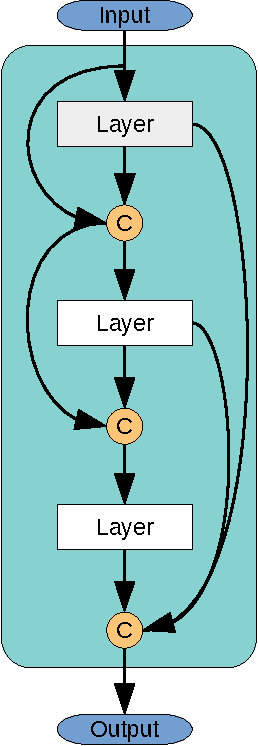
\includegraphics[width=0.23\linewidth]{./Figures/dense_block-crop.pdf}
	\caption{Representation of a Dense Block with three layers.}
	\label{fig:db}
\end{figure}



\begin{figure}[!t]
	\centering
	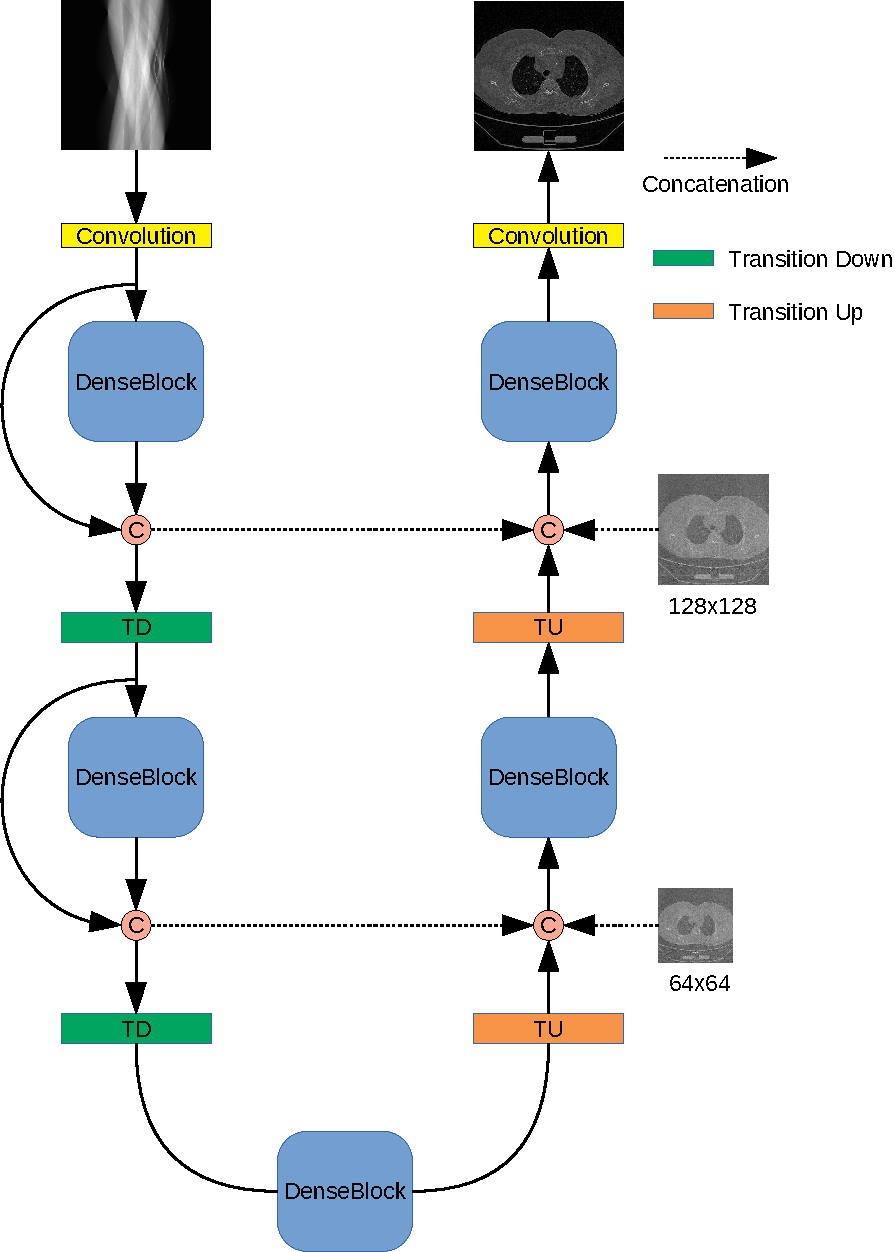
\includegraphics[width=.83\linewidth]{./Figures/densenet-crop.pdf}
	\caption{\ac{LRRCED}(D): Fully convolutional dense network with $\boldx_1$ at $64\times64$ and $\boldx_2$ at $128\times128$.}
	\label{fig:dn}
\end{figure}



\begin{table}[ht!]
	\centering
	\caption{Architecture Summary.}
	\label{table:1a}
	\begin{tabular}{||c||} 
		\hline
		Input (Sinogram), channels=1 \\ 
		\hline
		$3 \times 3$ Convolutions \\ 
		\hline
		DB (4 layers) + TD  \\ 
		\hline
		DB (5 layers) + TD    \\ 
		\hline
		DB (7 layers) + TD \\  
		\hline 
		DB (10 layers) + TD \\ 
		\hline
		DB (12 layers) + TD \\  
		\hline
		DB (15 layers)    \\  
		\hline
		TU + DB (12 layers) \\
		\hline
		TU + DB (10 layers) \\
		Concatenate $\boldx_1$  \\
		\hline
		TU + DB (7 layers) \\
		Concatenate $\boldx_2$  \\     
		\hline
		TU + DB (5 layers) \\
		\hline
		TU + DB (4 layers) \\
		\hline
		$1\times 1$ Convolution \\
		\hline
		Sigmoid     \\
		\hline  
		Output (Image), channels $=1$ \\
		\hline  
		
		
	\end{tabular}
	
\end{table}


\begin{figure}[!htbp]
	\centering
	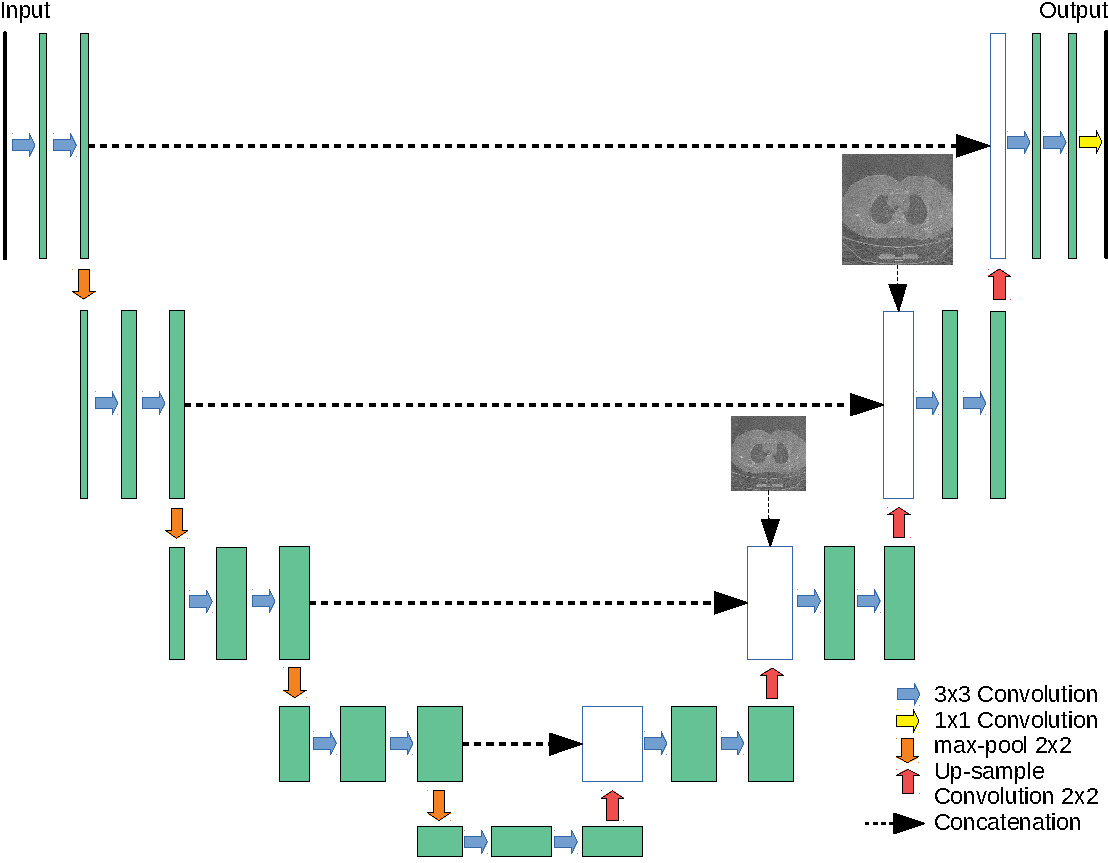
\includegraphics[width=0.8\linewidth]{./Figures/u_net-crop.pdf}
	\caption{\ac{LRRCED}(U): U-Net with $\boldx_1$ at $128\times128$ and $\boldx_2$ at $256\times256$.}
	\label{fig:un}
\end{figure}

\subsubsection{Loss Function}
The aim of a supervised data-driven image reconstruction task is to predict an image that is as close as possible to the \ac{GT} image. The appropriate loss function to achieve this is the \ac{MAE} which is defined as follows:
\begin{equation}
\mathrm{MAE}(\boldx^\star, \boldxhat) = \frac{1}{m}   \sum_{j=1}^m |x^\star_j - \hat{x}_j|
\end{equation}
where $\boldx^\star =  [x_1^\star, \dots , x_m^\star]^\top \in \mathbb{R}^m$ and $\boldxhat= [\hat{x}_1, \dots , \hat{x}_m]^\top \in \mathbb{R}^m$ are respectively the true image and predicted image.

In order to improve the resolution of reconstructed images, many deep learning approaches have used the perceptual loss as proposed by \cite{johnson2016perceptual}. This loss uses a pre-trained neural network to extract features from the predicted image and the \ac{GT}. It can be defined as follows:

\begin{equation}
P_k(\boldx^\star,\boldxhat) =  |[\mathrm{VGG16}]_k(\boldx^\star) - [\mathrm{VGG16}]_k( \boldxhat)|, \quad k =1,\dots,5 \,  
\end{equation}
where $[\mathrm{VGG16}]_k(\boldx^\star)$ and $[\mathrm{VGG16}]_k( \boldxhat)$ are the features extracted from block $k$ of the $\mathrm{VGG16}$ neural network \cite{simonyan2014very} with respectively the \ac{GT} and the predicted image as inputs. The features extracted from higher layers of the neural network contain generic information (edges, contrast, etc.) while the deeper layers have finer task-specific details. The VGG16 network was pre-trained on Image-Net data \cite{deng2009imagenet} which is far from a medical context. Hence, the higher-level generic features were found to be more relevant for the task of medical image reconstruction. We observed that using extracted features from two different levels, namely Block 1 and Block 3, of the VGG16 network proved to be most effective. 

The final loss function that was used for training both the aforementioned networks is defined as follows: 
\begin{equation}\label{eq:loss}
\mathcal{L}(\boldx^\star,\boldxhat) = \alpha\mathrm{MAE}(\boldx^\star, \boldxhat)+\beta(P_{1}(\boldx^\star,\boldxhat)+P_{3}(\boldx^\star,\boldxhat))
\end{equation}
where $P_{1}$ and $P_{3}$ are perceptual loss from the extracted features of the two different blocks above-mentioned, $\alpha$ and $\beta$ are weights which were set to $0.5$ and $10$ during the training phase.  


\section{Dataset}
The data used in this work is from the \ac{Lung} \cite{Lung20,clark2013cancer}. Details of the dataset are given in Table~\ref{table:2a}. The images in this dataset were reconstructed using \ac{FBP} on full-angular coverage measurement data. We used the ASTRA toolbox \cite{van2016fast}, for data processing to create the projection-image pairs.  A fan-beam geometry with a source to detector distance at $1500$ mm and source to the center of the rotation at $1000$ mm were considered. The number of detectors was set to $700$ and the number of angles was varied to generate different levels of sparsity ($N_\mathrm{a}=60,90$ and $120$). The noise-free projection data were obtained using the Beer-Lambert law \eqref{eq:CT} with an input emission intensity of $10^5$. The final projection data were obtained by adding Poisson noise (i.e., \eqref{eq:poisson}) to the noise-free projection data. We finally generated the \ac{FBP} estimates from the noise-added sparse-projections which were used in training the networks as explained previously. Sample images from the dataset are shown in Figure~\ref{fig:data}. 



\begin{table}[ht!]
	\caption{Dataset Description}
	\label{table:2a}
	\centering
	\begin{tabular}{||c|c||} 
		\hline
		Dataset Statistics &  \\ [0.5ex] 
		\hline
		Modalities & CT, PET   \\ 
		\hline
		Number of Participants  & 355  \\
		\hline
		Number of Studies  & 436  \\
		\hline
		Number of Series & 1295 \\ 
		\hline
		Number of 2-D Image slices & 251,135 \\ 
		\hline
		PET Matrix size & 200 \\ 
		\hline
		CT Matrix size & 512 \\ 
		\hline
		
	\end{tabular}
	
\end{table}

\begin{figure}[!htbp]
	\centering
	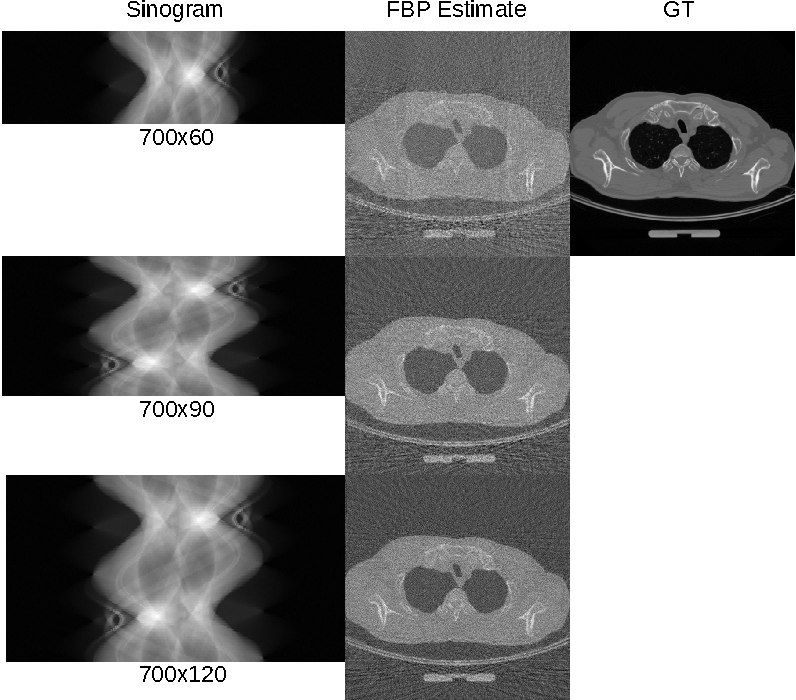
\includegraphics[width=0.8\linewidth]{./Figures/data-crop.pdf}
	\caption{Samples from the dataset: Sinograms with different sparse-view configurations along with their corresponding \ac{FBP} estimate.}
	\label{fig:data}
\end{figure}


\section{Training}

We implemented the architectures described in the previous section using TensorFlow \cite{abadi2016tensorflow} and Keras \cite{chollet2015keras}. A subset of the dataset consisting of 22,000 \ac{2D} \ac{CT} images was used in this study. We then split the data into 20,000 images for training and 2,000 images for testing. The sinograms and \ac{FBP} estimates were generated using the ASTRA toolbox as described above. The sinograms were resized to $512 \times 512$ to ensure symmetry with the images for easier training of the network. The \ac{FBP} estimates $\boldxhat_1$ and $\boldxhat_2$ were resized to the resolutions required for concatenation to the proposed networks. The neural networks were independently trained for each of the sparse-view settings with $N_\mathrm{a}=60,90$ and $120$. The choice of $\boldx_1$ and $\boldx_2$ were at $64\times64$ and $128\times128$ resolutions for \ac{LRRCED}(D) and $128\times128$ and $256\times256$ resolutions for \ac{LRRCED}(U). The networks were trained for 25 epochs with Adam optimizer with a decay of $10^{-4}$.


\section{Quantitative Analysis:}

The metrics used for evaluating the reconstructed images were \ac{SSIM} and \ac{PSNR}. They are defined as follows:
\begin{equation}
\mathrm{SSIM}(\boldx^\star,\boldx) = \frac{(2\mu_{\boldx^\star}\mu_{\boldx}+c_{1})(2\sigma_{\boldx^\star\boldx}+c_{2})}{(\mu_{\boldx^\star}^2+\mu_{\boldx}^2+c_{1})(\sigma_{\boldx^\star}^2+\sigma_{\boldx}^2+c_{2})}   
\end{equation}
where $\mu_{\boldx^\star}$ and $\mu_{\boldx}$ are the mean of $\boldx^\star$ and $\boldx$ respectively, $\sigma_{\boldx^\star}^2$ and $\sigma_{\boldx}^2$ are the variance of $\boldx^\star$ and $\boldx$, $\sigma_{\boldx^\star\boldx}$ is the covariance between $\boldx^\star$ and $\boldx$ , $c_{1}=(k_{1}L)^2$ and $c_{2}=(k_{2}L)^2$ where $k_{1}=0.01$ and $k_{2}=0.03$ by default,
\begin{equation}
\mathrm{PSNR} = 20\log_{10}\left(\frac{L-1}{\mathrm{RMSE}}\right)
\end{equation}
where $L$ is the maximum intensity in the image and \ac{RMSE} is given by
\begin{equation}
%    \mathrm{RMSE}(Y_\mathrm{true},Y_\mathrm{predicted}) = \sqrt{\frac{1}{n}   \sum_{i=1}^{n} (Y_\mathrm{true}^i-Y_\mathrm{predicted}^i)^2} 
\mathrm{RMSE}(\boldx^\star,\boldxhat) = \sqrt{\frac{1}{m}   \sum_{j=1}^{m} (x^\star_j-\xhat_j )^2} \, .
\end{equation}



\section{Comparative Analysis}

The  \ac{LRRCED} method was compared with a post-processing deep learning-based approach, namely FBP-ConvNet \cite{jin2017deep}, and a \ac{PWLS}-\ac{TV} solver for the model-based iterative \ac{CT} reconstruction \cite{tang2009performance}. We trained FBP-ConvNet on a set of 20,000 noisy, artifact-ridden \ac{FBP} image and \ac{GT} pairs. This network was trained for 25 epochs. 

\section{Results} \label{sec:results}

\subsection{Experimental Results}

Figure~\ref{fig:d_ang} shows the images reconstructed with \ac{LRRCED}(D) for various degrees of sparsity in the projections. Also given below each image is the \ac{SSIM} and \ac{PSNR} w.r.t. \ac{GT}. The region enclosed in the yellow box is further zoomed in for clearer inspection. As the sparsity in the views reduces, the \ac{SSIM} and \ac{PSNR} also improve. Similarly in Figure~\ref{fig:u_ang}, we show the images reconstructed with \ac{LRRCED}(U). Similar to the previous case, we observe improvements in the metrics as the sparsity decreases. 

In Figure~\ref{fig:res_60} and Figure~\ref{fig:res_90} we present a comparison of reconstructed images with different algorithms with 60 views and 90 views respectively. The top row consists of the \ac{GT} and the proposed \ac{LRRCED}(D) and \ac{LRRCED}(U) approaches. The second row consists of FBP-ConvNet, \ac{PWLS}-\ac{TV} iterative method and \ac{FBP}. The region highlighted in yellow is zoomed and corresponding images are displayed in the third and fourth rows. These methods are quantitatively compared in Table~\ref{table:3} and Table~\ref{table:4}. We observe that the deep learning methods perform better than the iterative and analytical methods. The proposed approach has the best metrics for projections with 90 views. The deep learning-based methods have similar metrics in the 60-view scenario. The intensity line profiles of the regions marked in red in Figure~\ref{fig:res_60} and Figure~\ref{fig:res_90} are plotted in Figure~\ref{fig:ip_60} and Figure~\ref{fig:ip_90} respectively. In accordance with the metrics tabulated in Table~\ref{table:3} and Table~\ref{table:4}, we find that the plots of deep learning-based methods are very close to that of the \ac{GT}. Even though the proposed approach with typical \acp{CED} performs a task which is more complex than denoising, the metrics indicate that the quality has not deteriorated compared to a standard post-processing approach. The inclusion of perceptual loss in \ref{eq:loss} was to improve the sharpness of the reconstructed images. This is indeed reflected in the images predicted by the proposed approach but we also observe some artifacts (regularly spaced white dots) in the images (especially for 60 views).

\begin{figure}[!htbp]
	\centering
	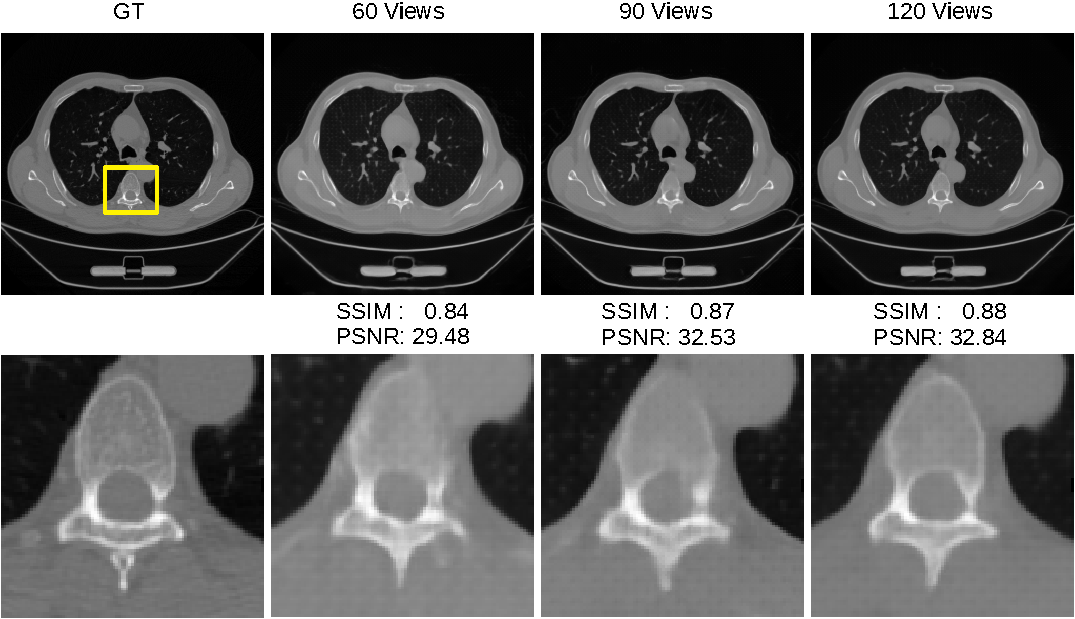
\includegraphics[width=0.8\linewidth]{./Figures/views_dense-crop.pdf}
	\caption{Images reconstructed with LRR-CED(D) approach with different sparse-view configurations, i.e., projections with $N_\mathrm{a}=60,90$ and $120$.}
	\label{fig:d_ang}
\end{figure}


\begin{figure}[!htbp]
	\centering
	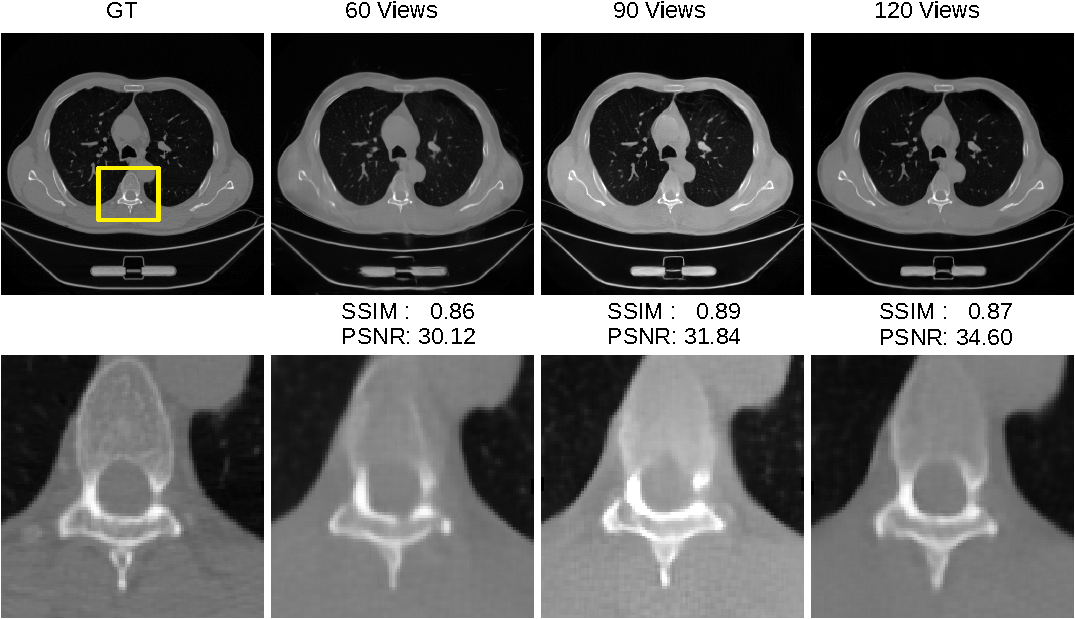
\includegraphics[width=0.8\linewidth]{./Figures/views_unet-crop.pdf}
	\caption{Images reconstructed with LRR-CED(U) approach with different Sparse-View configurations, i.e., projections with $N_\mathrm{a}=60,90$ and $120$.}
	\label{fig:u_ang}
\end{figure}


\begin{table}[ht!]
	\centering
	\caption{Quantitative comparison of various reconstruction algorithms with \ac{SSIM} and \ac{PSNR} for projections with 60 views}
	\label{table:3a}
	\begin{tabular}{||c|c|c|c|c|c||} 
		\hline
		Metric & FBP & PWLS-TV & FBP & \ac{LRRCED} & \ac{LRRCED}  \\ %[0.5ex] 
		&     &         & ConvNet & (D) & (U) \\
		\hline\hline
		SSIM & $0.16$ & $0.66$ & $0.85$ & $0.84$ & $0.87$ \\ 
		PSNR & $11.57$ & $28.23$ & $31.52$ & $29.48$ & $30.12$ \\   
		\hline  
		
		\hline  
	\end{tabular}
	
\end{table}

\begin{table}[ht!]
	\centering
	\caption{Quantitative comparison of various reconstruction algorithms with \ac{SSIM} and \ac{PSNR} for projections with 90 views}
	\label{table:4a}
	\begin{tabular}{||c|c|c|c|c|c||} 
		\hline
		Metric & FBP & PWLS-TV & FBP & \ac{LRRCED} & \ac{LRRCED}  \\ %[0.5ex] 
		&     &         & ConvNet & (D) & (U) \\
		\hline\hline
		SSIM & $0.19$ & $0.72$ & $0.81$ & $0.88$ & $0.89$ \\ 
		PSNR & $13.57$ & $30.21$ & $31.45$ & $32.53$ & $31.84$ \\   
		\hline  
		
		\hline  
	\end{tabular}
	
\end{table}



\begin{figure}[!t]
	\centering
	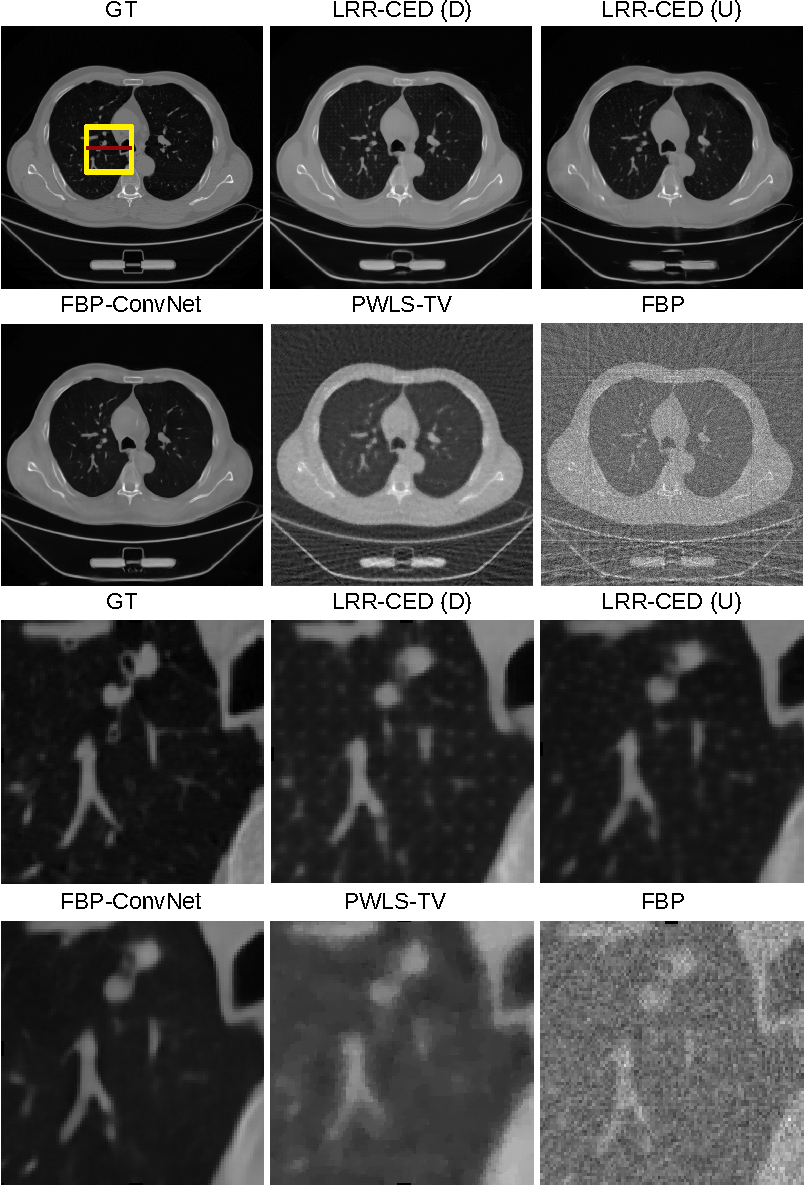
\includegraphics[width=1.0\linewidth]{./Figures/results1-crop.pdf}
	\caption{Comparative analysis for 60 views: From the top left, we have \ac{GT} image, reconstructions with \ac{LRRCED}(D) and \ac{LRRCED}(U). In the second row reconstructed images with FBP-ConvNet, PWLS-TV and \ac{FBP}. }
	\label{fig:res_60}
\end{figure}

\begin{figure}[!t]
	\centering
	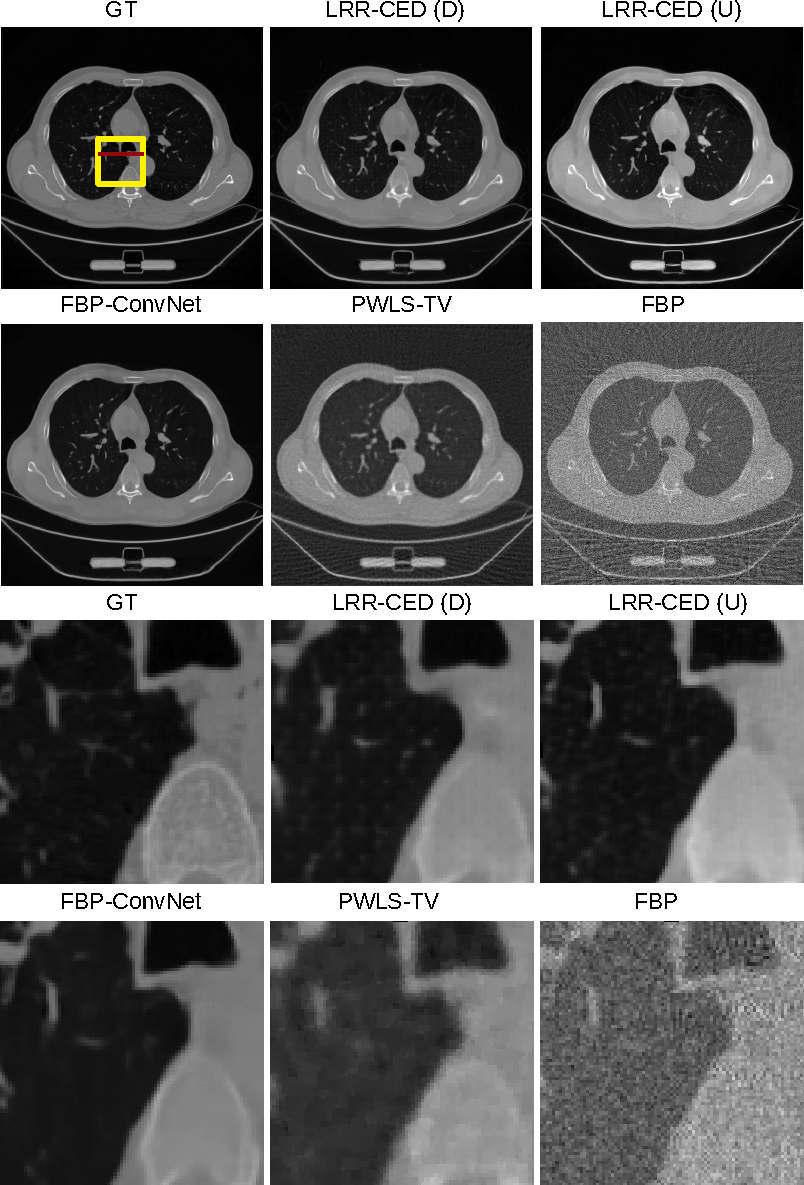
\includegraphics[width=1.0\linewidth]{./Figures/result2-crop.pdf}
	\caption{Comparative analysis for 90 views: From the top we have \ac{GT} image, reconstructions with \ac{LRRCED}(D) and \ac{LRRCED}(U). In the second row reconstructed images with FBP-ConvNet, PWLS-TV and \ac{FBP}.}
	\label{fig:res_90}
\end{figure}

\begin{figure}[!h]
	\centering
	\begin{tikzpicture}[scale=1] 
	\begin{axis}[
	% title=X-ray source Energy: $140$ keV,
	mark options={mark size = 3pt},
	xlabel={Distance (in pixels)},
	ylabel={Normalized Attenuation (mm$^{-1}$)},
	xmin = 200,
	xmax = 300,
	grid = major,
	legend columns=2,
	legend cell align=left,
	legend entries={PWLS-TV,\ac{GT},\ac{LRRCED}(D),\ac{LRRCED}(U),FBP-ConvNet},
	% legend entries={MCAOL,CAOL, Huber, TV, },
	legend style={at={(0.5,1.2)},anchor=north}
	]
	
	\addplot[color=blue, style={thick}] table[x=Distance, y=PWLS-TV] {./Plots/Fig11.txt};
	\addplot[color=green, style={thick}] table[x=Distance, y=GT] {./Plots/Fig11.txt};
	\addplot[color=red, style={thick}] table[x=Distance, y=LRR-CED(D)] {./Plots/Fig11.txt};
	\addplot[color=magenta, style={thick}] table[x=Distance, y=LRR-CED(U)] {./Plots/Fig11.txt};
	\addplot[color=black, style={thick}] table[x=Distance, y=FBP-ConvNet] {./Plots/Fig11.txt};
	\end{axis}
	\end{tikzpicture}
	
	\caption{Intensity plot profile for the region marked in red from Figure~\ref{fig:res_60} for PWLS-TV, \ac{GT}, \ac{LRRCED}(D), \ac{LRRCED}(U) and FBP-ConvNet.}\label{fig:ip_60}
\end{figure}

\begin{figure}[!h]
	\centering
	\begin{tikzpicture}[scale=1] 
	\begin{axis}[
	% title=X-ray source Energy: $140$ keV,
	mark options={mark size = 3pt},
	xlabel={Distance (in pixels)},
	ylabel={Normalized Attenuation (mm$^{-1}$)},
	xmin = 200,
	xmax = 300,
	grid = major,
	legend columns=2,
	legend cell align=left,
	legend entries={PWLS-TV,\ac{GT},\ac{LRRCED}(D),\ac{LRRCED}(U),FBP-ConvNet},
	% legend entries={MCAOL,CAOL, Huber, TV, },
	legend style={at={(0.5,1.2)},anchor=north}
	]
	
	\addplot[color=blue, style={thick}] table[x=Distance, y=PWLS-TV] {./Plots/Fig10.txt};
	\addplot[color=green, style={thick}] table[x=Distance, y=GT] {./Plots/Fig10.txt};
	\addplot[color=red, style={thick}] table[x=Distance, y=LRR-CED(D)] {./Plots/Fig10.txt};
	\addplot[color=magenta, style={thick}] table[x=Distance, y=LRR-CED(U)] {./Plots/Fig10.txt};
	\addplot[color=black, style={thick}] table[x=Distance, y=FBP-ConvNet] {./Plots/Fig10.txt};
	\end{axis}
	\end{tikzpicture}
	
	\caption{Intensity plot profile for the region marked in red from Figure~\ref{fig:res_90} for PWLS-TV, \ac{GT}, \ac{LRRCED}(D), \ac{LRRCED}(U) and FBP-ConvNet.}\label{fig:ip_90}
\end{figure}


\subsection{Hyperparameter optimization}

Finding the optimal hyperparameters is an important aspect of training neural networks. The common hyperparameters in a typical \ac{CNN} are number of filters, number of layers, etc. These interdependent hyperparameters  determine the rate of convergence and require task-specific experimentation to arrive at the best possible configuration. The unique hyperparameters in our proposed approach are the resolutions of concatenated \ac{FBP} estimates. The number of training examples is another important component that varies depending on the task and the trainable parameters of the neural network selected for the task. In this section we discuss our experiments that determined the selection of these two important hyperparameters. 

\subsubsection{Concatenation Resolution Selection} \label{sec:concat}

To select the best possible configuration for concatenation in the proposed approach, we trained the networks with a fixed set of hyper-parameters and different combinations of concatenations. We discuss the results with \ac{LRRCED}(D) in this regard. The number of training samples were set to 10,000 for all the experiments. The training data were projections with 90 views, corresponding \ac{FBP} reconstructed images and the \ac{GT}. The training was done for 25 epochs. Each of the concatenation setting was evaluated on 5 test patients. The average \ac{SSIM} for each patient was plotted for each of the experiment setting. In Fig~\ref{fig:c1} we have the average \ac{SSIM} vs Patient plot for single concatenation at a specific resolution. Similarly Figure~\ref{fig:c2} consists of plots for double concatenation at two different resolutions. The double concatenation at $64\times64, 128\times128$ overall leads to the best metrics, thus becoming our choice for the experiments in this work. These results are tabulated in Table~\ref{table:5}.



\subsubsection{Training Examples Analysis}

One of the biggest challenges in any data driven algorithm is the selection of training examples required for the experiments. It is important to analyze this hyper-parameter as it serves as an important factor for the network to be reproducible and scalable. We varied the number of training examples for the best concatenation setting from the previous section and the 90-view scenario. The evaluation was similar to the previous experiment with the average \ac{SSIM} for 5 patients. The results from these experiments are tabulated in Table~\ref{table:6}. As seen in Figure~\ref{fig:tr}, the performance of the network improves along with the increase in the number of training examples. There is however a marginal difference in the performance of the network when trained with 20,000 or 30,000 training examples, hence making us choose 20,000 training examples as the optimum number for this hyper-parameter. The average \ac{SSIM} values across the test patients tend to get similar as the number of training examples increases.




\begin{table}[ht!]
	\centering
	\caption{Average \ac{SSIM} for different configurations of concatenations}
	\label{table:5}
	\begin{tabular}{||c|c|c|c|c|c||} 
		\hline
		Concatenated & \multicolumn{5}{c||}{Average \ac{SSIM}}  \\ \cline{2-6}%[0.5ex] 
		\ac{FBP} Resolution &   P1  &  P2     & P3 & P4 & P5 \\
		\hline\hline
		$(32\times32)$ & $0.82$ & $0.86$ & $0.88$ & $0.86$ & $0.80$ \\ 
		$(64\times64)$ & $0.85$ & $0.88$ & $0.90$ & $0.88$ & $0.82$ \\   
		$(128\times128)$ & $0.85$ & $0.87$ & $0.90$ & $0.89$ & $0.81$ \\   
		$(256\times256)$ & $0.58$ & $0.88$ & $0.85$ & $0.88$ & $0.79$ \\   
		$(512\times512)$ & $0.66$ & $0.78$ & $0.82$ & $0.75$ & $0.73$ \\   
		\hline
		$(32\times32,64\times64)$ & $0.83$ & $0.77$ & $0.80$ & $0.80$ & $0.68$ \\   
		$\mathbf{(64\times64,128\times128)}$ & $\mathbf{0.85}$ & $\mathbf{0.88}$ & $\mathbf{0.91}$ & $\mathbf{0.89}$ & $\mathbf{0.83}$ \\   
		$(128\times128,256\times256)$ & $0.67$ & $0.78$ & $0.83$ & $0.84$ & $0.70$ \\   
		\hline  
		
		\hline  
	\end{tabular}
	
\end{table}

\begin{table}[ht!]
	\centering
	\caption{Average \ac{SSIM} for different number of training examples}
	\label{table:6}
	\begin{tabular}{||c|c|c|c|c|c||} 
		\hline
		Number of Training  & \multicolumn{5}{c||}{Average \ac{SSIM}}  \\ \cline{2-6}%[0.5ex] 
		examples &   P1  &  P2     & P3 & P4 & P5 \\
		\hline\hline
		$1,000$ & $0.82$ & $0.79$ & $0.86$ & $0.85$ & $0.72$ \\ 
		$5,000$ & $0.84$ & $0.77$ & $0.86$ & $0.84$ & $0.69$ \\   
		$10,000$ & $0.85$ & $0.88$ & $0.91$ & $0.89$ & $0.83$ \\   
		$\mathbf{20,000}$ & $\mathbf{0.89}$ & $\mathbf{0.90}$ & $\mathbf{0.91}$ & $\mathbf{0.90}$ & $\mathbf{0.82}$ \\   
		$30,000$ & $0.89$ & $0.89$ & $0.90$ & $0.90$ & $0.82$ \\   
		\hline  
		
		\hline  
	\end{tabular}
	\vspace{.5cm}
\end{table}



\begin{figure}[!h]
	\centering
	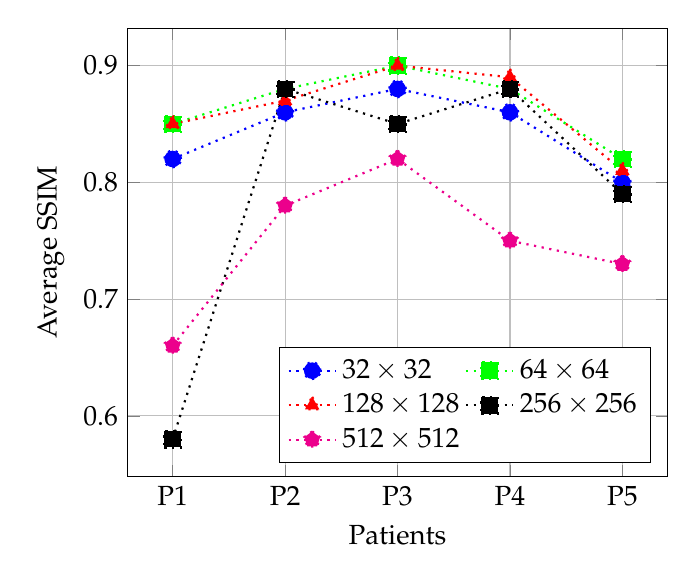
\begin{tikzpicture}[scale=1] 
	\begin{axis}[
	% title=X-ray source Energy: $140$ keV,
	mark options={mark size = 3pt},
	xlabel={Patients},
	ylabel={Average SSIM},
	xticklabels={,P1,P2,P3,P4,P5},
	grid = major,
	legend columns=2,
	legend cell align=left,
	legend entries={$32\times 32$,$64\times 64$,$128\times 128$,$256\times 256$,$512\times 512$},
	% legend entries={MCAOL,CAOL, Huber, TV, },
	legend style={legend pos=south east}
	]
	
	\addplot[color=blue, mark=*, style={thick,dotted}] coordinates   {(0,0.82)(10,0.86)(20,0.88)(30,0.86)(40,0.8)};
	\addplot[color=green, mark=square*, style={thick,dotted}] coordinates  {(0,0.85)(10,0.88)(20,0.9)(30,0.88)(40,0.82)};
	\addplot[color=red, mark=triangle*, style={thick,dotted}] coordinates  {(0,0.85)(10,0.87)(20,0.9)(30,0.89)(40,0.81)};
	\addplot[color=black, mark=square*, style={thick,dotted}] coordinates    {(0,0.58)(10,0.88)(20,0.85)(30,0.88)(40,0.79)};
	\addplot[color=magenta, mark=pentagon*, style={thick,dotted}] coordinates {(0,0.66)(10,0.78)(20,0.82)(30,0.75)(40,0.73)};
	
	\end{axis}
	\end{tikzpicture}
	
	\caption{Comparison of single concatenations for the particular case of 90 views evaluated with \ac{SSIM} on 5 different patients from the dataset. The best metrics are found with concatenation at $128\times 128$.}\label{fig:c1}
\end{figure}



\begin{figure}[!htbp]
	\centering
	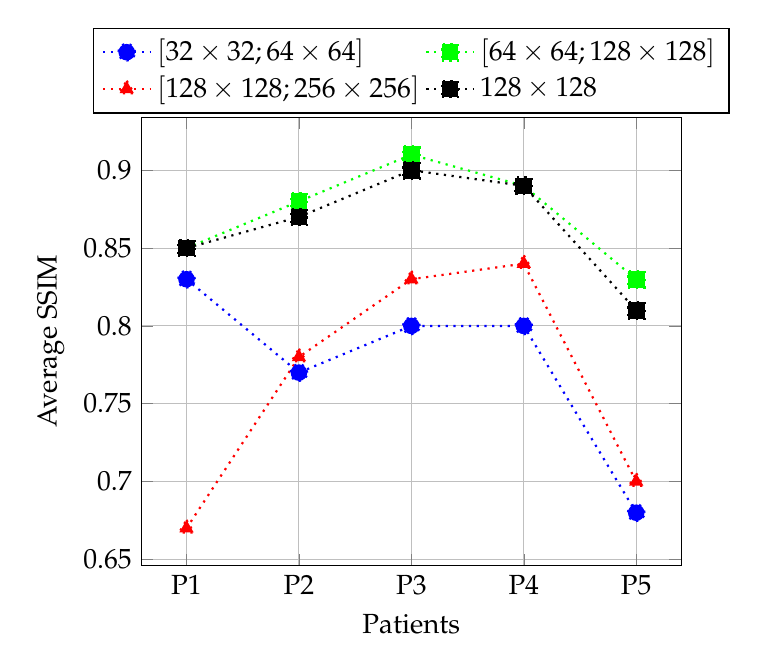
\begin{tikzpicture}[scale=1] 
	\begin{axis}[
	% title=X-ray source Energy: $140$ keV,
	mark options={mark size = 3pt},
	xlabel={Patients},
	ylabel={Average SSIM},
	xticklabels={,P1,P2,P3,P4,P5},
	grid = major,
	legend columns=2,
	legend cell align=left,
	legend entries={$[32\times 32 ; 64\times 64]$,$[64\times 64 ; 128\times 128]$,$[128\times 128 ; 256\times 256]$,$128\times 128$},
	% legend entries={MCAOL,CAOL, Huber, TV, },
	legend style={at={(0.5,1.2)},anchor=north}
	]
	
	\addplot[color=blue, mark=*, style={thick,dotted}] coordinates   {(0,0.83)(10,0.77)(20,0.8)(30,0.8)(40,0.68)};
	\addplot[color=green, mark=square*, style={thick,dotted}] coordinates  {(0,0.85)(10,0.88)(20,0.91)(30,0.89)(40,0.83)};
	\addplot[color=red, mark=triangle*, style={thick,dotted}] coordinates  {(0,0.67)(10,0.78)(20,0.83)(30,0.84)(40,0.7)};
	\addplot[color=black, mark=square*, style={thick,dotted}] coordinates    {(0,0.85)(10,0.87)(20,0.9)(30,0.89)(40,0.81)};
	
	\end{axis}
	\end{tikzpicture}
	
	\caption{Comparison of double concatenations for the particular case of 90 views evaluated with \ac{SSIM} on 5 different patients from the dataset. The best metrics are found with concatenations at $64\times 64$ and $128\times 128$ resolutions.}\label{fig:c2}
\end{figure}


\begin{figure}[!h]
	\centering
	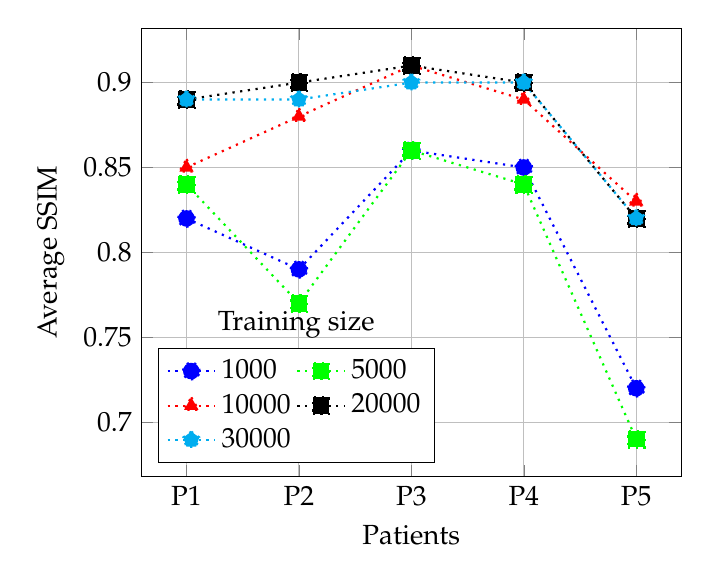
\begin{tikzpicture}[scale=1] 
	\begin{axis}[
	% title=X-ray source Energy: $140$ keV,
	mark options={mark size = 3pt},
	xlabel={Patients},
	ylabel={Average SSIM},
	xticklabels={,P1,P2,P3,P4,P5},
	grid = major,
	legend columns=2,
	legend cell align=left,
	legend entries={$1000$,$5000$,$10000$,$20000$,$30000$},
	% legend entries={MCAOL,CAOL, Huber, TV, },
	legend style={legend pos=south west,label=above:Training size}
	]
	
	\addplot[color=blue, mark=*, style={thick,dotted}] coordinates   {(0,0.82)(10,0.79)(20,0.86)(30,0.85)(40,0.72)};
	\addplot[color=green, mark=square*, style={thick,dotted}] coordinates  {(0,0.84)(10,0.77)(20,0.86)(30,0.84)(40,0.69)};
	\addplot[color=red, mark=triangle*, style={thick,dotted}] coordinates  {(0,0.85)(10,0.88)(20,0.91)(30,0.89)(40,0.83)};
	\addplot[color=black, mark=square*, style={thick,dotted}] coordinates    {(0,0.89)(10,0.9)(20,0.91)(30,0.9)(40,0.82)};
	\addplot[color=cyan, mark=pentagon*, style={thick,dotted}] coordinates {(0,0.89)(10,0.89)(20,0.9)(30,0.9)(40,0.82)};
	
	\end{axis}
	\end{tikzpicture}
	
	\caption{Comparison of Average \ac{SSIM} for 5 different Patient data for 90 views with varying number of training samples. The configuration of the network is the one with best performance from the analysis in Figure~\ref{fig:c1}. (concatenations at $64\times 64$ and $128\times 128$). }\label{fig:tr}
\end{figure}



\section{Discussion} \label{sec:discussion}

The use of deep learning architectures in the framework of medical image reconstruction is propelled by potentially faster reconstruction without compromising on the quality of the images. To this end, hybrid image reconstruction involving unrolled iterative algorithms with embedded deep learning architectures do not significantly reduce the reconstruction time. Hence, the use of deep learning architectures for either improving images from a fast analytic algorithm or direct reconstruction becomes more relevant for their incorporation into the image reconstruction pipeline. One significant problem for direct image reconstruction is the requirement of large and complex networks to learn the mapping from sinograms to images without the help of any reconstruction estimate. The networks used for post-processing on the other hand are simpler and relatively easy to train. In this work we attempted to use these post-processing networks for the direct image reconstruction task. We show that concatenating \ac{FBP} estimates at lower resolutions is sufficient to allow the network to learn the mapping from sinogram to image space. Through the use of two different networks with the concatenation approach we demonstrate that this idea can be applied to \acp{CED} in general.   

In the sparse-view \ac{CT} scenario artifact removal along with denoising increases the challenges of getting a clean well-resolved image. We observed that the use of traditional loss functions (L1 or L2) resulted in blurry images. To tackle this and to improve the sharpness of the images we used perceptual loss along with the standard L1 loss. The reconstructed images with our proposed \ac{LRRCED}(D) and \ac{LRRCED}(U) have higher \ac{SSIM} and \ac{PSNR} than images reconstructed with a traditional iterative algorithm. The evaluation metrics were very close to a standard post-processing deep learning method FBP-ConvNet. This similarity stems from the fact that the choice of networks used in our proposed work was inspired from post-processing \acp{CED}. The contribution in this work is the use of these networks to learn the mapping from sparse sinograms to images with the same amount of training examples, which is possible only with the proposed addition of the concatenations.  

We are currently exploring the possibility of using image estimates from earlier iterations of standard iterative algorithms while ensuring that the trade-off between time and image quality is not compromised. The use of other alternative architectures is also being explored to arrive at reconstructed images which perform significantly better than existing post-processing approaches. Finally, we are working on experiments with low-dose \ac{CT} and other tomographic reconstruction modalities to establish the adaptability of the proposed approach.  

\section{Conclusion} \label{sec:conclusion}

In this work we studied the use of fully convolutional encoder-decoder networks in direct sparse-\ac{CT} image reconstruction. We introduced a new approach that uses lower dimension \ac{FBP} estimates as concatenations to help the network learn the mapping from sinogram to image space. In the context of image reconstruction, we inject the information from the inverse of a \ac{CT} physical system (\ac{FBP} estimate) as a feature map in the decoder. We presented two variations of the proposed approach namely \ac{LRRCED}(D) using fully convolutional dense networks and \ac{LRRCED}(U) using U-Net. The proposed neural networks reconstruct images that are either better or are on par with traditional reconstruction algorithms and post-processing deep learning based approach (FBP-ConvNet). A single pass of a sparse sinogram through the network results in reconstructed images without the artifacts and noise which are severely present in the concatenated \ac{FBP} estimates. Finally, this idea of using task specific concatenations that enable one to have control over what the network learns, can be extended to various other problems in medical imaging. 


 

%----------------------------------------------------------------------------------------
%	THESIS CONTENT - APPENDICES
%----------------------------------------------------------------------------------------

\appendix % Cue to tell LaTeX that the following "chapters" are Appendices

% Include the appendices of the thesis as separate files from the Appendices folder
% Uncomment the lines as you write the Appendices

% Appendix A

\chapter{Frequently Asked Questions} % Main appendix title

\label{AppendixA} % For referencing this appendix elsewhere, use \ref{AppendixA}

\section{How do I change the colors of links?}

The color of links can be changed to your liking using:

{\small\verb!\hypersetup{urlcolor=red}!}, or

{\small\verb!\hypersetup{citecolor=green}!}, or

{\small\verb!\hypersetup{allcolor=blue}!}.

\noindent If you want to completely hide the links, you can use:

{\small\verb!\hypersetup{allcolors=.}!}, or even better: 

{\small\verb!\hypersetup{hidelinks}!}.

\noindent If you want to have obvious links in the PDF but not the printed text, use:

{\small\verb!\hypersetup{colorlinks=false}!}.

%\include{Appendices/AppendixB}
%\include{Appendices/AppendixC}

%----------------------------------------------------------------------------------------
%	BIBLIOGRAPHY
%----------------------------------------------------------------------------------------

\printbibliography[heading=bibintoc]

%----------------------------------------------------------------------------------------

\end{document}  
